\documentclass[11pt,a4paper,serbian,oneside]{book}
\usepackage[utf8]{inputenc}
\usepackage[T2A]{fontenc}
\usepackage{amsmath}
\usepackage{amssymb}
\usepackage{textcomp}
\usepackage{amsfonts}
\usepackage{graphicx}
%\usepackage{ucs}
\usepackage{listings}
\usepackage[serbianc]{babel}
%\usepackage{pdfsync}
\usepackage[left=2.5cm,right=2.5cm,top=2.5cm,bottom=2.5cm]{geometry}
\usepackage{float}
\usepackage{wrapfig}
\usepackage{color}
\usepackage{xcolor}
\usepackage{caption}
\usepackage{subcaption}
\usepackage{url}
\usepackage{fancyvrb}
\usepackage{verbatimbox}
\usepackage{listings,mdframed}% http://ctan.org/pkg/{listings,mdframed}
\usepackage[section]{placeins}
\usepackage[toc,acronym]{glossaries}
% Definisanje boja
\definecolor{lightgray}{rgb}{0.95, 0.95, 0.95}
\definecolor{darkgray}{rgb}{0.4, 0.4, 0.4}
\definecolor{purple}{rgb}{0.65, 0.12, 0.82}
\definecolor{ocherCode}{rgb}{1, 0.5, 0}
\definecolor{blueCode}{rgb}{0, 0, 0.93} % #0000EE -> rgb(0, 0, 238)
\definecolor{greenCode}{rgb}{0, 0.6, 0} % #009900 -> rgb(0, 153, 0) 

\colorlet{punct}{red!60!black}
%\definecolor{background}{HTML}{EEEEEE}
\definecolor{delim}{RGB}{20,105,176}
\colorlet{numb}{magenta!60!black}

% Komanda za horizontal ruler
\newcommand{\HRule}{\rule{\linewidth}{0.5mm}}
\renewcommand*\arraystretch{1.5}

\def\zn{,\kern-0.09em,}
%
% Definicija fiksiranih reci
%
\addto\captionsserbian{%
 \def\prefacename{Предговор}%
 \def\refname{Списак литературе}%
 \def\abstractname{Сажетак}%
 \def\bibname{Литература}%
 \def\chaptername{Глава}%
 \def\appendixname{Додатак}%
 \def\contentsname{Садржај}%
 \def\listfigurename{Списак слика}%
 \def\listtablename{Списак табела}%
 \def\indexname{Регистар}%
 \def\figurename{Слика}%
 \def\tablename{Табела}%
 \def\partname{Део}%
 \def\enclname{Прилози}%
 \def\ccname{Копије}%
 \def\headtoname{Прима}%
 \def\pagename{Страна}%
 \def\seename{Види}%
 \def\alsoname{Види такође}%
 \def\proofname{Доказ}%
 \def\glossaryname{Речник непознатих речи}
 \def\contentsname{Садржај}%
 }%

%
% Podesavanja paketa za listinge
%
\renewcommand\lstlistingname{Листинг}

\lstdefinelanguage{CSS}{
  morekeywords={accelerator,azimuth,background,background-attachment,
    background-color,background-image,background-position,
    background-position-x,background-position-y,background-repeat,
    behavior,border,border-bottom,border-bottom-color,
    border-bottom-style,border-bottom-width,border-collapse,
    border-color,border-left,border-left-color,border-left-style,
    border-left-width,border-right,border-right-color,
    border-right-style,border-right-width,border-spacing,
    border-style,border-top,border-top-color,border-top-style,
    border-top-width,border-width,bottom,caption-side,clear,
    clip,color,content,counter-increment,counter-reset,cue,
    cue-after,cue-before,cursor,direction,display,elevation,
    empty-cells,filter,float,font,font-family,font-size,
    font-size-adjust,font-stretch,font-style,font-variant,
    font-weight,height,ime-mode,include-source,
    layer-background-color,layer-background-image,layout-flow,
    layout-grid,layout-grid-char,layout-grid-char-spacing,
    layout-grid-line,layout-grid-mode,layout-grid-type,left,
    letter-spacing,line-break,line-height,list-style,
    list-style-image,list-style-position,list-style-type,margin,
    margin-bottom,margin-left,margin-right,margin-top,
    marker-offset,marks,max-height,max-width,min-height,
    min-width,-moz-binding,-moz-border-radius,
    -moz-border-radius-topleft,-moz-border-radius-topright,
    -moz-border-radius-bottomright,-moz-border-radius-bottomleft,
    -moz-border-top-colors,-moz-border-right-colors,
    -moz-border-bottom-colors,-moz-border-left-colors,-moz-opacity,
    -moz-outline,-moz-outline-color,-moz-outline-style,
    -moz-outline-width,-moz-user-focus,-moz-user-input,
    -moz-user-modify,-moz-user-select,orphans,outline,
    outline-color,outline-style,outline-width,overflow,
    overflow-X,overflow-Y,padding,padding-bottom,padding-left,
    padding-right,padding-top,page,page-break-after,
    page-break-before,page-break-inside,pause,pause-after,
    pause-before,pitch,pitch-range,play-during,position,quotes,
    -replace,richness,right,ruby-align,ruby-overhang,
    ruby-position,-set-link-source,size,speak,speak-header,
    speak-numeral,speak-punctuation,speech-rate,stress,
    scrollbar-arrow-color,scrollbar-base-color,
    scrollbar-dark-shadow-color,scrollbar-face-color,
    scrollbar-highlight-color,scrollbar-shadow-color,
    scrollbar-3d-light-color,scrollbar-track-color,table-layout,
    text-align,text-align-last,text-decoration,text-indent,
    text-justify,text-overflow,text-shadow,text-transform,
    text-autospace,text-kashida-space,text-underline-position,top,
    unicode-bidi,-use-link-source,vertical-align,visibility,
    voice-family,volume,white-space,widows,width,word-break,
    word-spacing,word-wrap,writing-mode,z-index,zoom},
  morestring=[s]{:}{;},
  sensitive,
  morecomment=[s]{/*}{*/}
}

\lstdefinestyle{nonumbers}
{numbers=none}


\lstdefinelanguage{HTML5}{
    sensitive=true,
    keywords={%
    % JavaScript
    typeof, new, true, false, catch, function, return, null, catch, switch, var, if, in, while, do, else, case, break,
    % HTML
    html, title, meta, style, head, body, script, canvas, div
    % CSS
    border:, transform:, -moz-transform:, transition-duration:, transition-property:,
    transition-timing-function:
    },
    % http://texblog.org/tag/otherkeywords/
    otherkeywords={<, >, \/},   
    ndkeywords={class, export, boolean, throw, implements, import, this},   
    comment=[l]{//},
    % morecomment=[s][keywordstyle]{<}{>},  
    morecomment=[s]{/*}{*/},
    morecomment=[s]{<!}{>},
    morestring=[b]',
    morestring=[b]",    
    alsoletter={-},
    alsodigit={:}
}

\lstdefinelanguage{json}{
    basicstyle=\normalfont\ttfamily,
    numbers=left,
    numberstyle=\scriptsize,
    stepnumber=1,
    numbersep=8pt,
    showstringspaces=false,
    breaklines=true,
    frame=lines,
    %backgroundcolor=\color{background},
    literate=
     *{0}{{{\color{numb}0}}}{1}
      {1}{{{\color{numb}1}}}{1}
      {2}{{{\color{numb}2}}}{1}
      {3}{{{\color{numb}3}}}{1}
      {4}{{{\color{numb}4}}}{1}
      {5}{{{\color{numb}5}}}{1}
      {6}{{{\color{numb}6}}}{1}
      {7}{{{\color{numb}7}}}{1}
      {8}{{{\color{numb}8}}}{1}
      {9}{{{\color{numb}9}}}{1}
      {:}{{{\color{punct}{:}}}}{1}
      {,}{{{\color{punct}{,}}}}{1}
      {\{}{{{\color{delim}{\{}}}}{1}
      {\}}{{{\color{delim}{\}}}}}{1}
      {[}{{{\color{delim}{[}}}}{1}
      {]}{{{\color{delim}{]}}}}{1},
}


\lstset {
	basicstyle=\ttfamily\tiny
	numbers=left,
	numberstyle=\tiny,
	%stepnumber=2,
	numbersep=5pt,
	extendedchars=true,
	breaklines=true,
	keywordstyle=\color{blue},
	frame=b,
    % Code design
	stringstyle=\color{white}\ttfamily,
    identifierstyle=\color{black},
    keywordstyle=\color{blue}\bfseries,
    ndkeywordstyle=\color{greenCode}\bfseries,
    commentstyle=\color{darkgray}\ttfamily,
    % Code    
	tabsize=2,    
	showspaces=false,
	showtabs=false,
	xleftmargin=17pt,
	framexleftmargin=14pt,
	framexrightmargin=3pt,
	framexbottommargin=4pt,
	framextopmargin=0pt,
	%backgroundcolor=\color{lightgray},
	showstringspaces=false,
    extendedchars=true,
    breaklines=true    
}


\makeatletter
%% define a caption format; if the caption
%% is the default (\relax), the separator is
%% not printed; as long as no caption text
%% starts with \relax, this will work
\DeclareCaptionFormat{alsoempty}{%
  #1\if\relax\expandafter\noexpand\lst@caption\else#2#3\fi}
\makeatother
%% set this format as the default for lstlisting
\captionsetup[lstlisting]{format=alsoempty}

\lstset{%
    % Basic design
    basicstyle=\fontsize{10}{10}\selectfont\ttfamily,
    frame=l,
    % Line numbers
    xleftmargin={0.75cm},
    numbers=left,
    stepnumber=1,
    firstnumber=1,
    numberfirstline=true,
    % Code design
    identifierstyle=\color{black},
    keywordstyle=\color{blue}\bfseries,
    ndkeywordstyle=\color{greenCode}\bfseries,
    stringstyle=\color{ocherCode}\ttfamily,
    commentstyle=\color{darkgray}\ttfamily,
    % Code
    language={HTML5},
    tabsize=2,
    showtabs=false,
    showspaces=false,
    showstringspaces=false,
    extendedchars=true,
    breaklines=true,
    caption=\relax
    %captionpos=b
}

\lstloadlanguages {
	% Check Documentation for further languages ...
	%[Visual]Basic
	%Pascal
	C,
	%C++
	%Java,
	%XML,
	%HTML5
}

%
% Podesavanje okvira listinga
%
\DeclareCaptionFont{black}{\color{black}}
\DeclareCaptionFormat{listing}{\colorbox[cmyk]{0, 0, 0,0.01}{\parbox{\textwidth}{\hspace{12pt}#1#2#3}}}
\captionsetup[lstlisting]{format=listing,labelfont=black,textfont=black, singlelinecheck=false, margin=0pt, font={bf,footnotesize} }

\makeglossaries
 
\newglossaryentry{MDS}
{
    name=MDS,
    description={Metadata Server}
}
\newglossaryentry{MDT}
{
    name=MDT,
    description={Metadata Target}
}

\newglossaryentry{OSS}
{
    name=OSS,
    description={Object Storage Servers}
}

\newglossaryentry{OST}
{
    name=OST,
    description={Object Storage Target}
}

\newglossaryentry{NFS}
{
    name=NFS,
    description={Network File Sistem}
}

\newglossaryentry{HPC}
{
    name=HPC,
    description={High-Performance Computing}
}

\newglossaryentry{API}
{
    name=API,
    description={Application Programming Interface}
}

\newglossaryentry{MDC}
{
    name=MDC,
    description={Metadata Client}
}
\newglossaryentry{OSC}
{
    name=OSC,
    description={Object Storage Client}
}
\newglossaryentry{MGC}
{
    name=MGC,
    description={Management Client}
}
\newglossaryentry{NAL}
{
    name=NAL,
    description={Network Abstraction Layers}
}

\newglossaryentry{LNET}
{
    name=LNET,
    description={Lustre Networking}
}
\newglossaryentry{LVM}
{
    name=LVM,
    description={Logical Volume Management}
}
\newglossaryentry{ACL}
{
    name=ACL,
    description={Access Control Lists}
}
\newglossaryentry{PDSH}
{
    name=PDSH,
    description={Parallel Distributed SHell}
}
\newglossaryentry{SSH}
{
    name=SSH,
    description={Secure SHell}
}
\newglossaryentry{NTP}
{
    name=NTP,
    description={Network Time Protocol}
}
\newglossaryentry{SELinux}
{
    name=SELinux,
    description={Security-Enhanced Linux}
}
\newglossaryentry{SNMP}
{
    name=SNMP,
    description={Simple Network Management Protocol}
}
\newglossaryentry{MPI}
{
    name=MPI,
    description={Message-Passing Interface}
}
\newglossaryentry{RMA}
{
    name=RMA,
    description={Remote Memory Access}
}
\newglossaryentry{PVM}
{
    name=PVM,
    description={Parallel Virtual Machine }
}
\newglossaryentry{NAT}
{
    name=NAT,
    description={Network Address Translation }
}
%
% Pocetak dokumenta
%
\begin{document}




%
% Naslovna stranica
%

\begin{titlepage}

\begin{center}

% Gornji deo stranice

\includegraphics[width=0.25\textwidth]{logo-pmf.pdf}\\[1cm]    

\textsc{\LARGE Институт за математику и информатику
\\ Природно-математички факултет
\\ Универзитет у Крагујевцу}\\[1.5cm]

\textsc{\Large Мастер рад}\\[0.5cm]

% Naslov
\HRule \\[0.4cm]
{ \huge \bfseries MPI-2 стандард и Lustre фајл систем}\\[0.4cm]

\HRule \\[1.5cm]

% Autor i mentor
\begin{minipage}{0.4\textwidth}
\begin{flushleft} \large
\emph{Студент:}\\
Ненад Ацковић
\end{flushleft}
\end{minipage}
\begin{minipage}{0.4\textwidth}
\begin{flushright} \large
\emph{Професор:} \\
др Милош Ивановић
\end{flushright}
\end{minipage}

\vfill

% Dno stranice
{\large Септембар 2015.}

\end{center}

\end{titlepage}


\tableofcontents
\newpage

\printglossary[style=long,title={Скраћенице}]

\newpage

\chapter{ \textit{Увод} }
%\section{Увод}
Овај рад као примарни циљ поставља проучавање могућности \textit{Lustre} фајл система у унапређењу рада кластера високих перформанси, као и користи од паралелних улазно излазних операција дефинисаних \gls{MPI}-2 стандардом.
\textit{Lustre} паралелни фајл систем има предност над осталим (секвенцијалним) системима услед могућности обављања улазно-излазних операција у паралелном маниру. Са друге стране, MPI-2 представља индустријски стандард за развој паралелних програма, а његове имплементације подржавају паралелно читање и писање на уређаје масовне меморије. У циљу сагледавања начина да се побољшају укупне перформансе локалног кластера \textit{Мedflow}, упоређују се брзине читања и писања података у фајлове који се налазе како на \textit{Lustre}, тако и на NFS  фајл систему.

Кластер високих перформанси (\textit{\gls{HPC}}) представља скуп рачунара умрежених коришћењем локалне мрежне инфраструктуре, помоћу које међусобно комуницирају. Коришћење специфичне програмске подршке даје висок степен интеграције рачунара, омогућава њихов координирани заједнички рад и претвара их ефективно у јединствен вишепроцесорски систем који користи дистрибуирану меморију.

За истраживачке радове који захтевају обимне математичке прорачуне данас се углавном користе паралелни програми који на кластеру високих перформанси рашчлањују проблем на више рачунарских процесора. Тиме се време добијања резултата знатно смањује у односу на време потребно за добијање резултата на једном процесору, понекад за више редова величине. Најефективнији начин је употреба поменутог MPI стандарда за развој паралелних програма. На Универзитету у Крагујевцу постоји неколико HPC кластера, али ни један од њих не поседује паралелни фајл систем. Та чињеница у појединим случајевима употребе може да доведе до озбиљног пада перформанси. На срећу, први кластер са паралелним фајл системом постављен је недавно у истраживачко развојном центру за биоинжееринг у Крагујевцу. Након иницијалне инсталације HPC кластера, дошло се на идеју да се истраже реалне могућности и употребна вредност новоинсталираног \textit{Lustre} система, што и представља основну мотивацију за израду овог рада.
 
У раду су дата тестирања брзина извршавања операција фајл система помоћу програма \textit{Iozone}, \textit{dd} и \textit{Game of Life}. Под претпоставком да постоји разлика у брзини улазно/излазних операција ових фајл система, анализирају се добијени резултати тестирања и на основу њих се утврђује који је погоднији за који домен употребе.

\newpage

\chapter{ \textit{Lustre} }
\section{Увод}

\textit{Lustre}   систем је бесплатан, дистрибуиран, паралелни фајл систем развијен од стране \textit{Sun Microsystems Inc}.  \textit{Lustre}  систем је дизајниран и имплементиран тако да смањи  или потпуно неутралише уска грла пређашњих паралелних фајл система. Централна компонента   \textit{Lustre}  система је дељени фајл систем за кластере.  \textit{Lustre}  је тренутно доступан за Linux оперативне системе и омогућава \textbf{UNIX®} фајл систем окружење.  \textit{Lustre}  архитектура се користи за више врста кластера. Користи се у седам од десет највећих кластера високих перфоманси у свету који имају хиљаде клијента, петабајте складишта и хиљаде  гигабајта у секунди У/И операција. Скалабилност коју нуди   \textit{Lustre}  учинила га је погодним алатом у оквиру истраживања нафте и гаса, у производњи као и у финансијском сектору. Са корисним побољшањима подршци у оквиру  \textit{Lustre}  мреже (\textit{LNET}) и софтверима који управљају  \textit{Lustre}  фајл системом, коришћење  \textit{Lustre}  фајл система би требало да буде још шире. Скалабилност   \textit{Lustre}  система смањује потребу за одвојеним фајл системима, на пример креирање једног фајл система за један кластер или још неефикасније један фајл систем за сваки \gls{NFS} фајл сервер. Ово доводи до предности управљања складиштем података, избегавајући вишеструке копије података на више фајл система. Главни  \gls{HPC} центри због тога захтевају много мање складишта података са   \textit{Lustre}  фајл системом него са другим системима. Проток или капацитет може се лако подесити после инсталације кластера, уколико се дода нови сервер. Како је   \textit{Lustre}  бесплатан систем, усвојен је од стране једног броја рачунарских компанија и интегрисан је њиховим понудама. У циљу једноставне инсталације   \textit{Lustre}  фајл система, \textit{Red Hat} и \textit{Novell} (\textit{SUSE}) нуде закрпе кернела својих дистрибуција.  \textit{Lustre}  архитектура први пут је развијена 1999. године, а 2003. године је објављена верзија 1.0 и одмах је искоришћена на великом броју кластера високих перформанси. Коришћење   \textit{Lustre}  система такође је утицало и на побољшање перформанси \textit{Linux ext3} фајл система.


\newpage
\section{Компоненте  \textit{Lustre}  фајл система}
\subsection{Основне компоненте}
\textit{Lustre} фајл систем се састоји од следећих основних компоненти(слика 2.1):
\begin{itemize}
\item
\textbf{Management Server(MGS)} 
 Чувa информације o конфигурацијама за све \textit{Lustre} системе у кластерy. Сваки \textit{Lustre} клијент контактира MGS да пружи информације. MGS захтева сопствени диск за складиштење. Међутим, постоји одредба која омогућава дељење MGS дискa (\zn ко-лоцирање") са једним MDT-ом. MGS се не сматра \zn делом" индивидуалног фајл система, већ пружа информације о конфигурацији за \textit{Lustre} компоненте.
 
\item 
\textbf{Metadata Server (\gls{MDS})} 
 MDS сервер чине метаподаци ускладиштени у један или више MDT сервера који су на располагању \textit{Lustre} клијентима. Сваки MDS  управља именима фајлова и директоријумима \textit{Lustre} система и обезбеђује мрежни захтев за руковање једним или више локалних MDT-а.

\item 
\textbf{Metadata Target (\gls{MDT})} 
 MDT чувa метаподатаке (као што су имена фајлова, директоријума, дозвола и распоред фајлова) на MDS-у. Сваки фајл систем има по један MDT. MDT на дељивом фајл систему може бити доступан многим MDS серверима, мада само један заправо треба да га користи. Уколико дође до грешке на MDT-у, MDS може аутоматски преузети његову улогу и ставити се на располагање клијентима. Ова могућност се назива MDS \textit{ failover}.

\item 
\textbf{Object Storage Servers (\gls{OSS})} 
 OSS обезбеђују улазно/излазне операције, као и захтеве за један или више локалних OST-а. Обично OSS опслужује између 2 и 8 OST-а, од којих један OST може имати до 16 TB складишног простора.  MDT, OST и \textit{Lustre} клијенти могу се покренути истовремено на једном чвору. Међутим, најзаступљенија конфигурација је да се MDT инсталира на одвојеном чвору, са једним или више OST-а на сваком OSS чвору.

\item 
\textbf{Object Storage Target (\gls{OST})} 
 OST чува податке (делове корисничних фајлова) на једном или више OSS-а. Један \textit{Lustre} фајл систем може имати више OST-а, од којих сваки опслужује део фајла. Није нужно да се један фајл налази на једном OST-у. У циљу оптимизације перформанси, фајл може бити расподељен на много OST-а. Logical Object Volume (LOV) управља деловима датотека на вишеструким OST.

\item 
\textbf{Lustre клијенти} 
 Lustre клијенти су рачунари који по покретању \textit{Lustre} програма омогућавају подизање партиције \textit{Lustre} система. \textit{Lustre} програм се састоји од окружења између \textit{Linux Virtul File System-a} и \textit{Lustre} сервера. Сваки клијент се састоји од: \textit{Metadata Client (\gls{MDC})}, \textit{Object Storage Client (\gls{OSC})} и \textit{Management Client (\gls{MGC})}. Група OSC се налази у једном LOV. Радећи здружено, OSC  омогућава  транспарентан приступ фајл систему. Клијенти који подижу \textit{Lustre} фајл систем виде један кохерентан и синхронизован фајл систем све време. Различити клијенти могу да уписују различите делове истoг фајла истовремено, док остали клијенти могу да читају из фајла.
\end{itemize}

\subsection{\textit{Lustre} Умрежавање (\gls{LNET})}

Lustre умрежавање (LNET) је \textit{\gls{API}} који управља мета подацима и улазно/излазним подацима за системске сервере и клијенте. LNET подржава више хетерогених окружења на клијентима и серверима. LNET комуницира са више врста мрежа преко \textit{Network Abstraction Layers (\gls{NAL})}. Lustre систему су на располагању већи број мрежа, укључујући \textit{Infiniband}, \textit{TCP/IP}, \textit{Qуadrics Elan}, \textit{Myrinet (MX and GM)} и \textit{Cray}.  Код кластера са \textit{Lustre} системом, сервери и клијенти комуницирају са дрyгом врстом мреже која се зове \textit{Lustre Networking (LNET)}, док су складишта MDS and OSS повезана традиционалним SAN технологијама.

\paragraph*{Кључне карактеристике \textit{Lustre} мреже}
\begin{itemize}
\item
RDMA - подршка мрежа као што су \textit{Elan}, \textit{Myrinet} и \textit{InfiniBand}.

\item
Подршка за много чешће коришћене типове мрежа попут \textit{InfiniBand} и \textit{TCP/IP}.

\item
Својства високе доступности и опоравка омогућавају транспарентан опоравак сервера.

\item
Истовремена доступност више мрежних типова са рутирањем између њих.
\end{itemize}

\begin{figure}[h!]
  \centering
      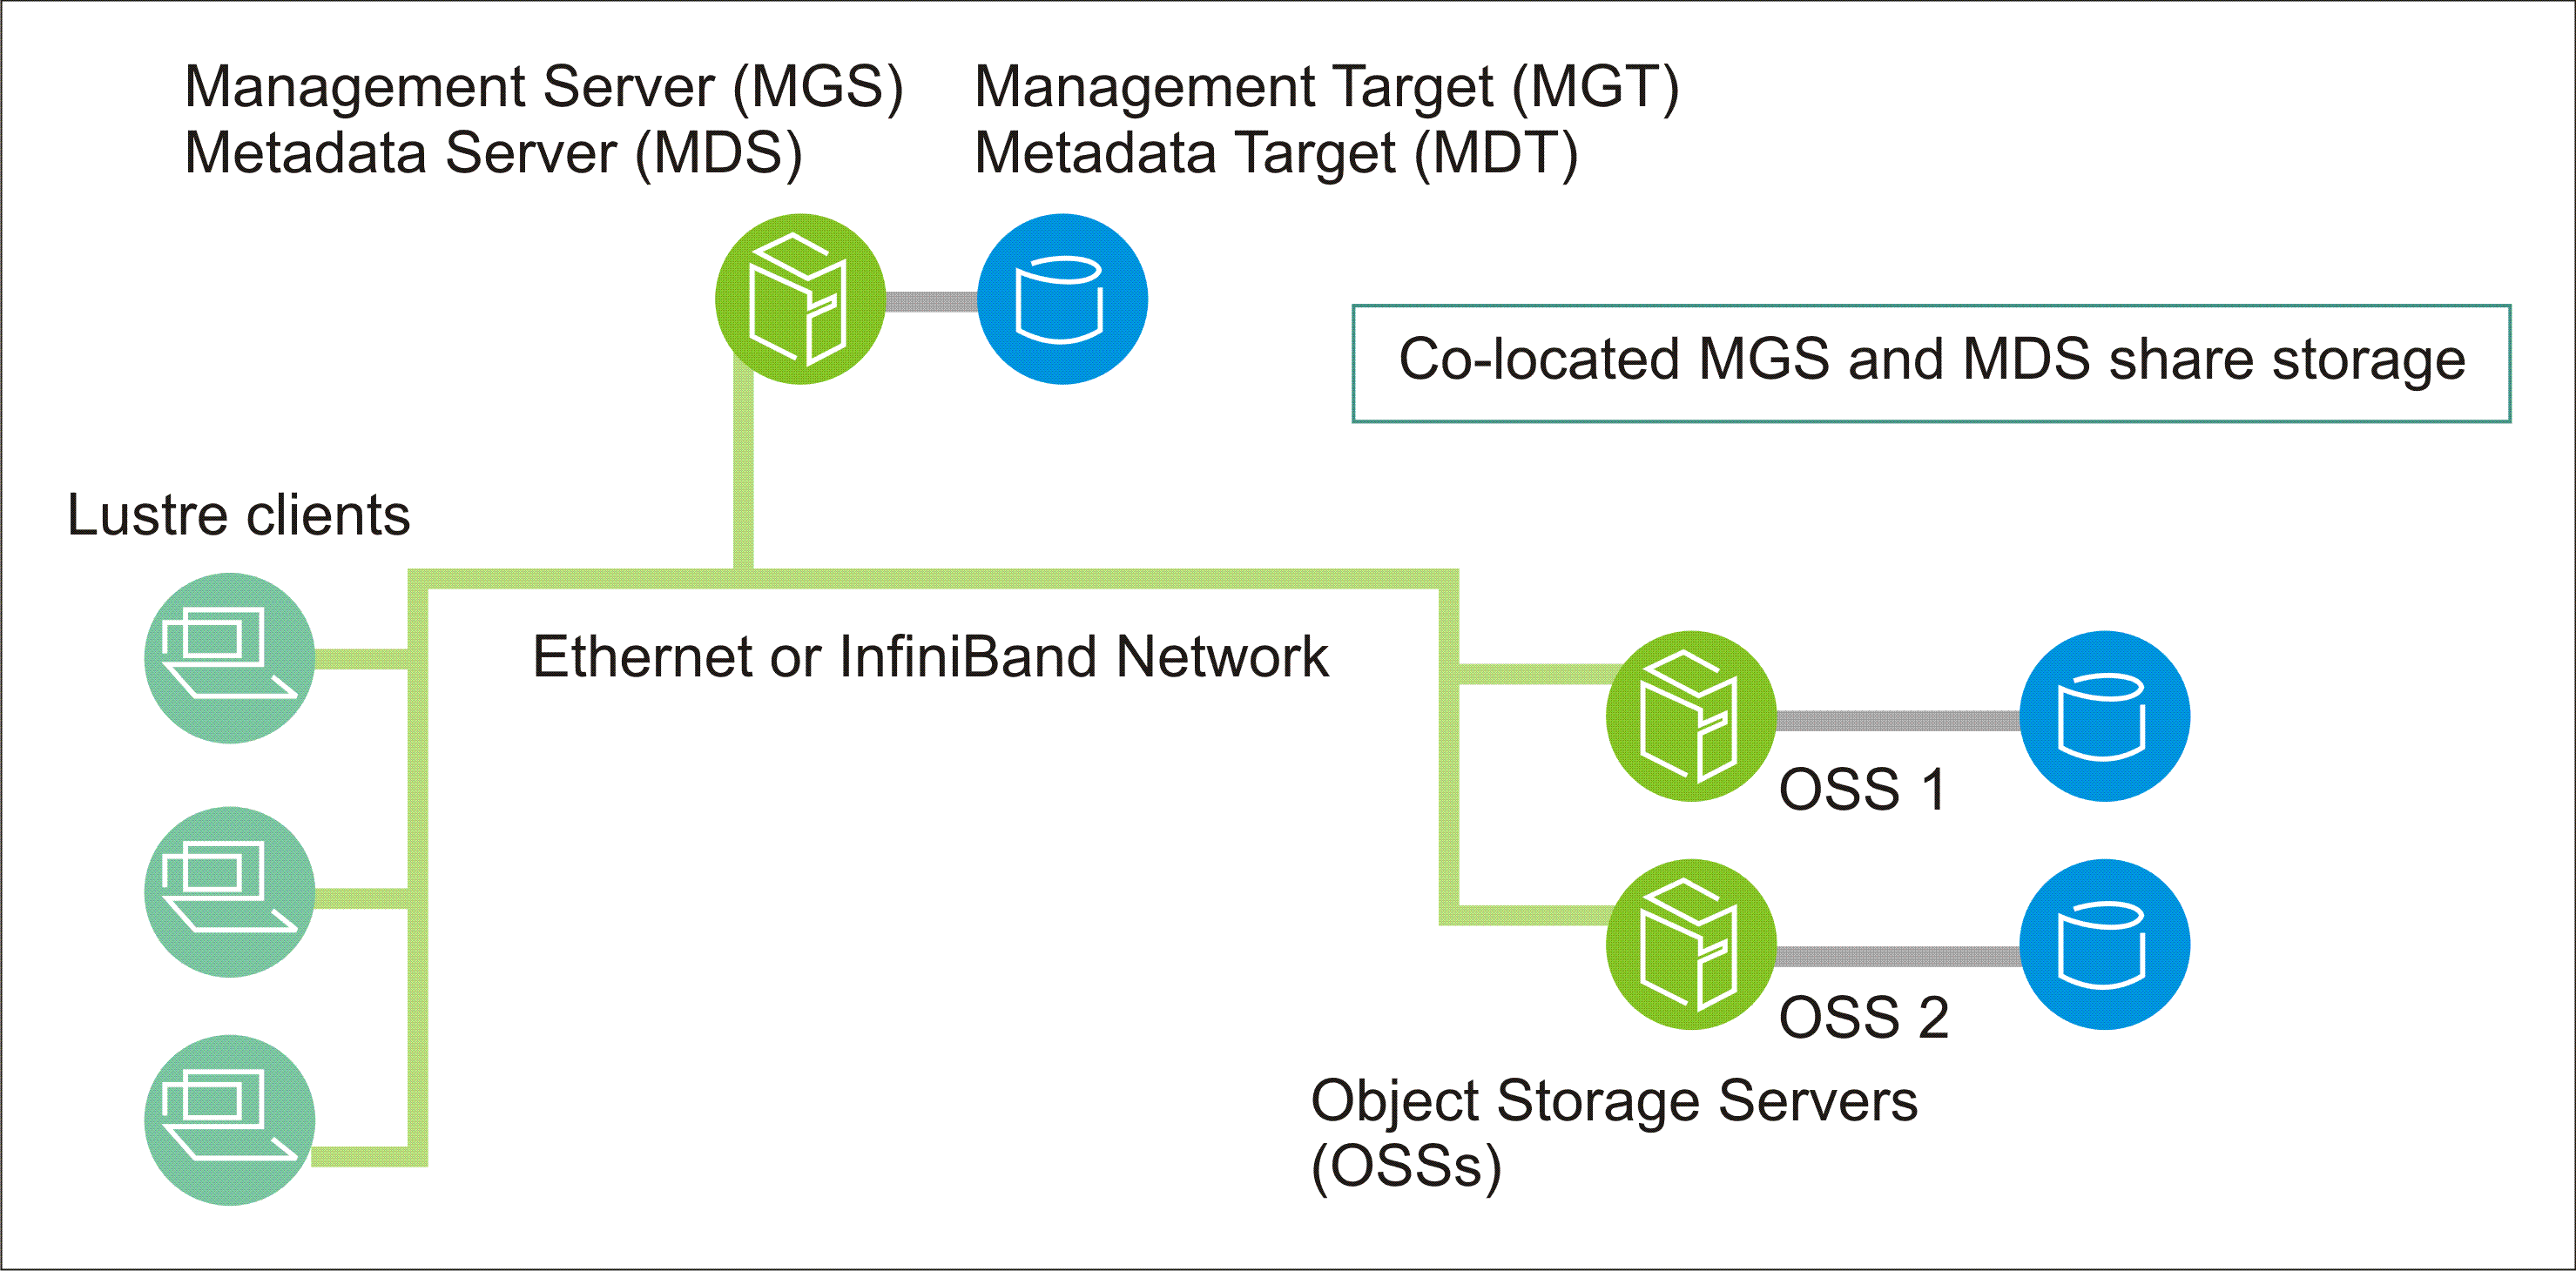
\includegraphics[width=1\textwidth]{slike/lustre.png}
  \caption{\textit{Lustre} компоненте}
\end{figure}




\section{Фајлови у   \textit{Lustre} систему}
Традиционални UNIX фајл системи користе чворове, који садрже спискове редних бројева блокова
где се чувају подаци о  фајлу за дати чвор. Слично томе, за сваки фајл у   \textit{Lustre} систему фајлова,
један чвор постоји на MDT-у. Међутим, у   \textit{Lustre} систему чвор на MDT није показивач на блок података, већ показује на један или више објеката коју су у вези са фајловима(слика 2.2). Ови објекти су датотеке на OST и садрже податке.

\begin{figure}[h!]
  \centering
      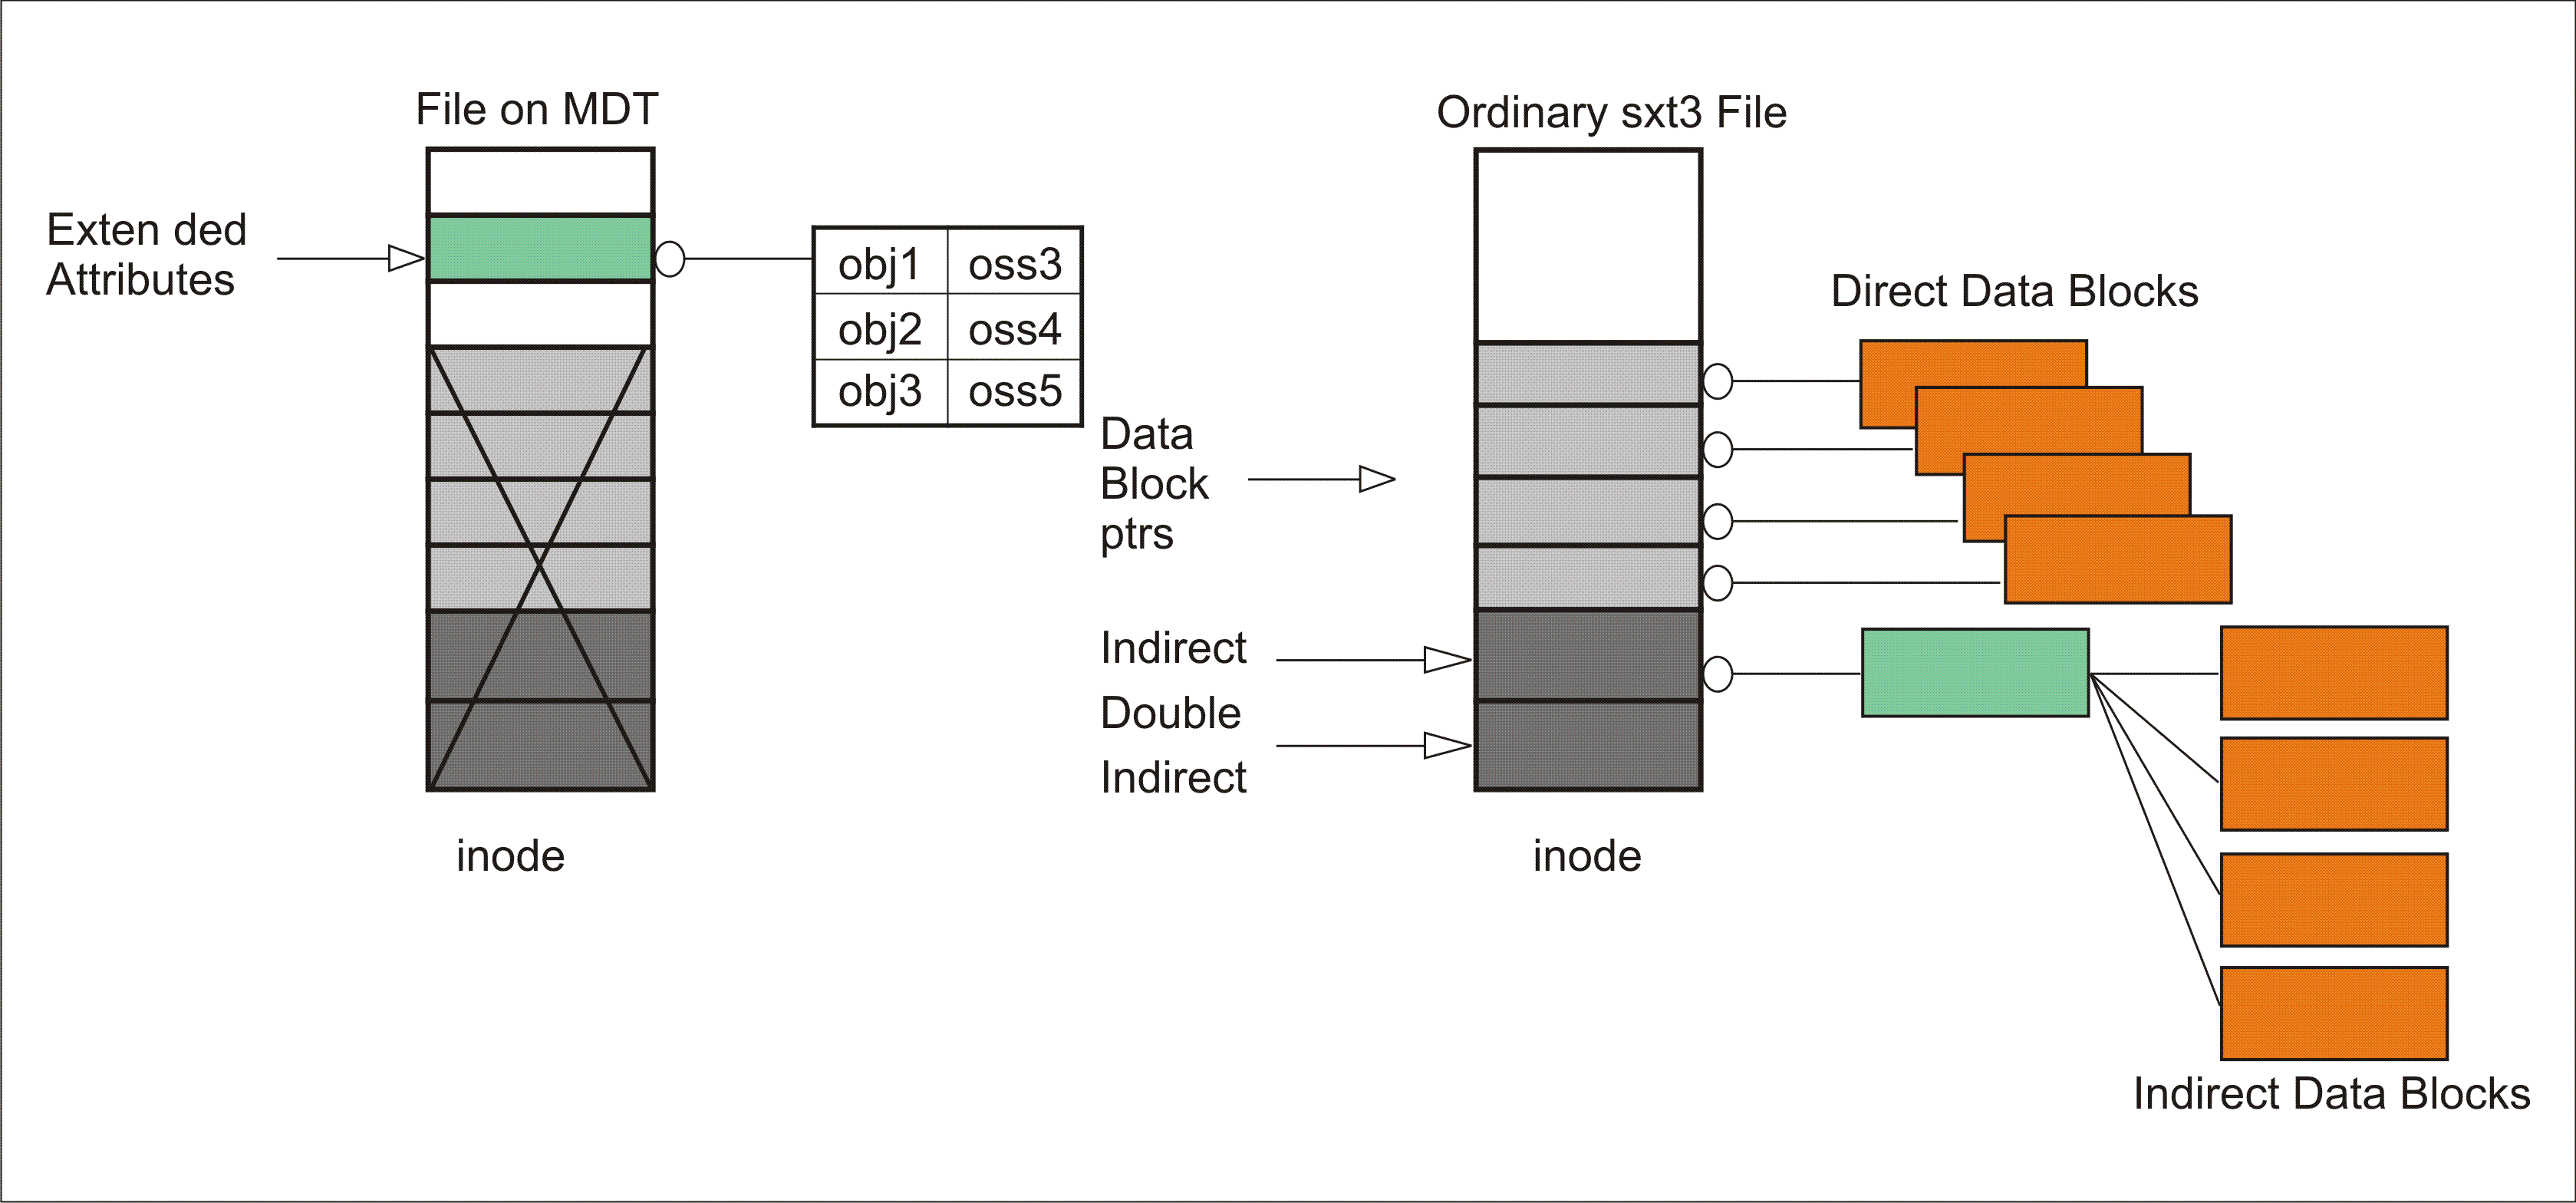
\includegraphics[width=1\textwidth]{slike/lustre_files.png}\\[1cm]
  \caption{Разлика измeђу MDS и ext3 чворова}
\end{figure}
\newpage

Уколико је само један објекат повезан са MDS чвор, тај објекат садржи све податке
у том систему. Када је више од једног објекта повезано, подаци у фајлу 
су подељени широм објекта. MDS зна распоред сваког фајла, број и локацију дела фајла. 
Клијенти добијају изглед фајла из MDS. Када клијент изврши  У/И операцију на делу фајла, 
фајл комуницира директно са релевантним OST-ом(слика 2.3). 

\begin{figure}[h!]
  \centering
      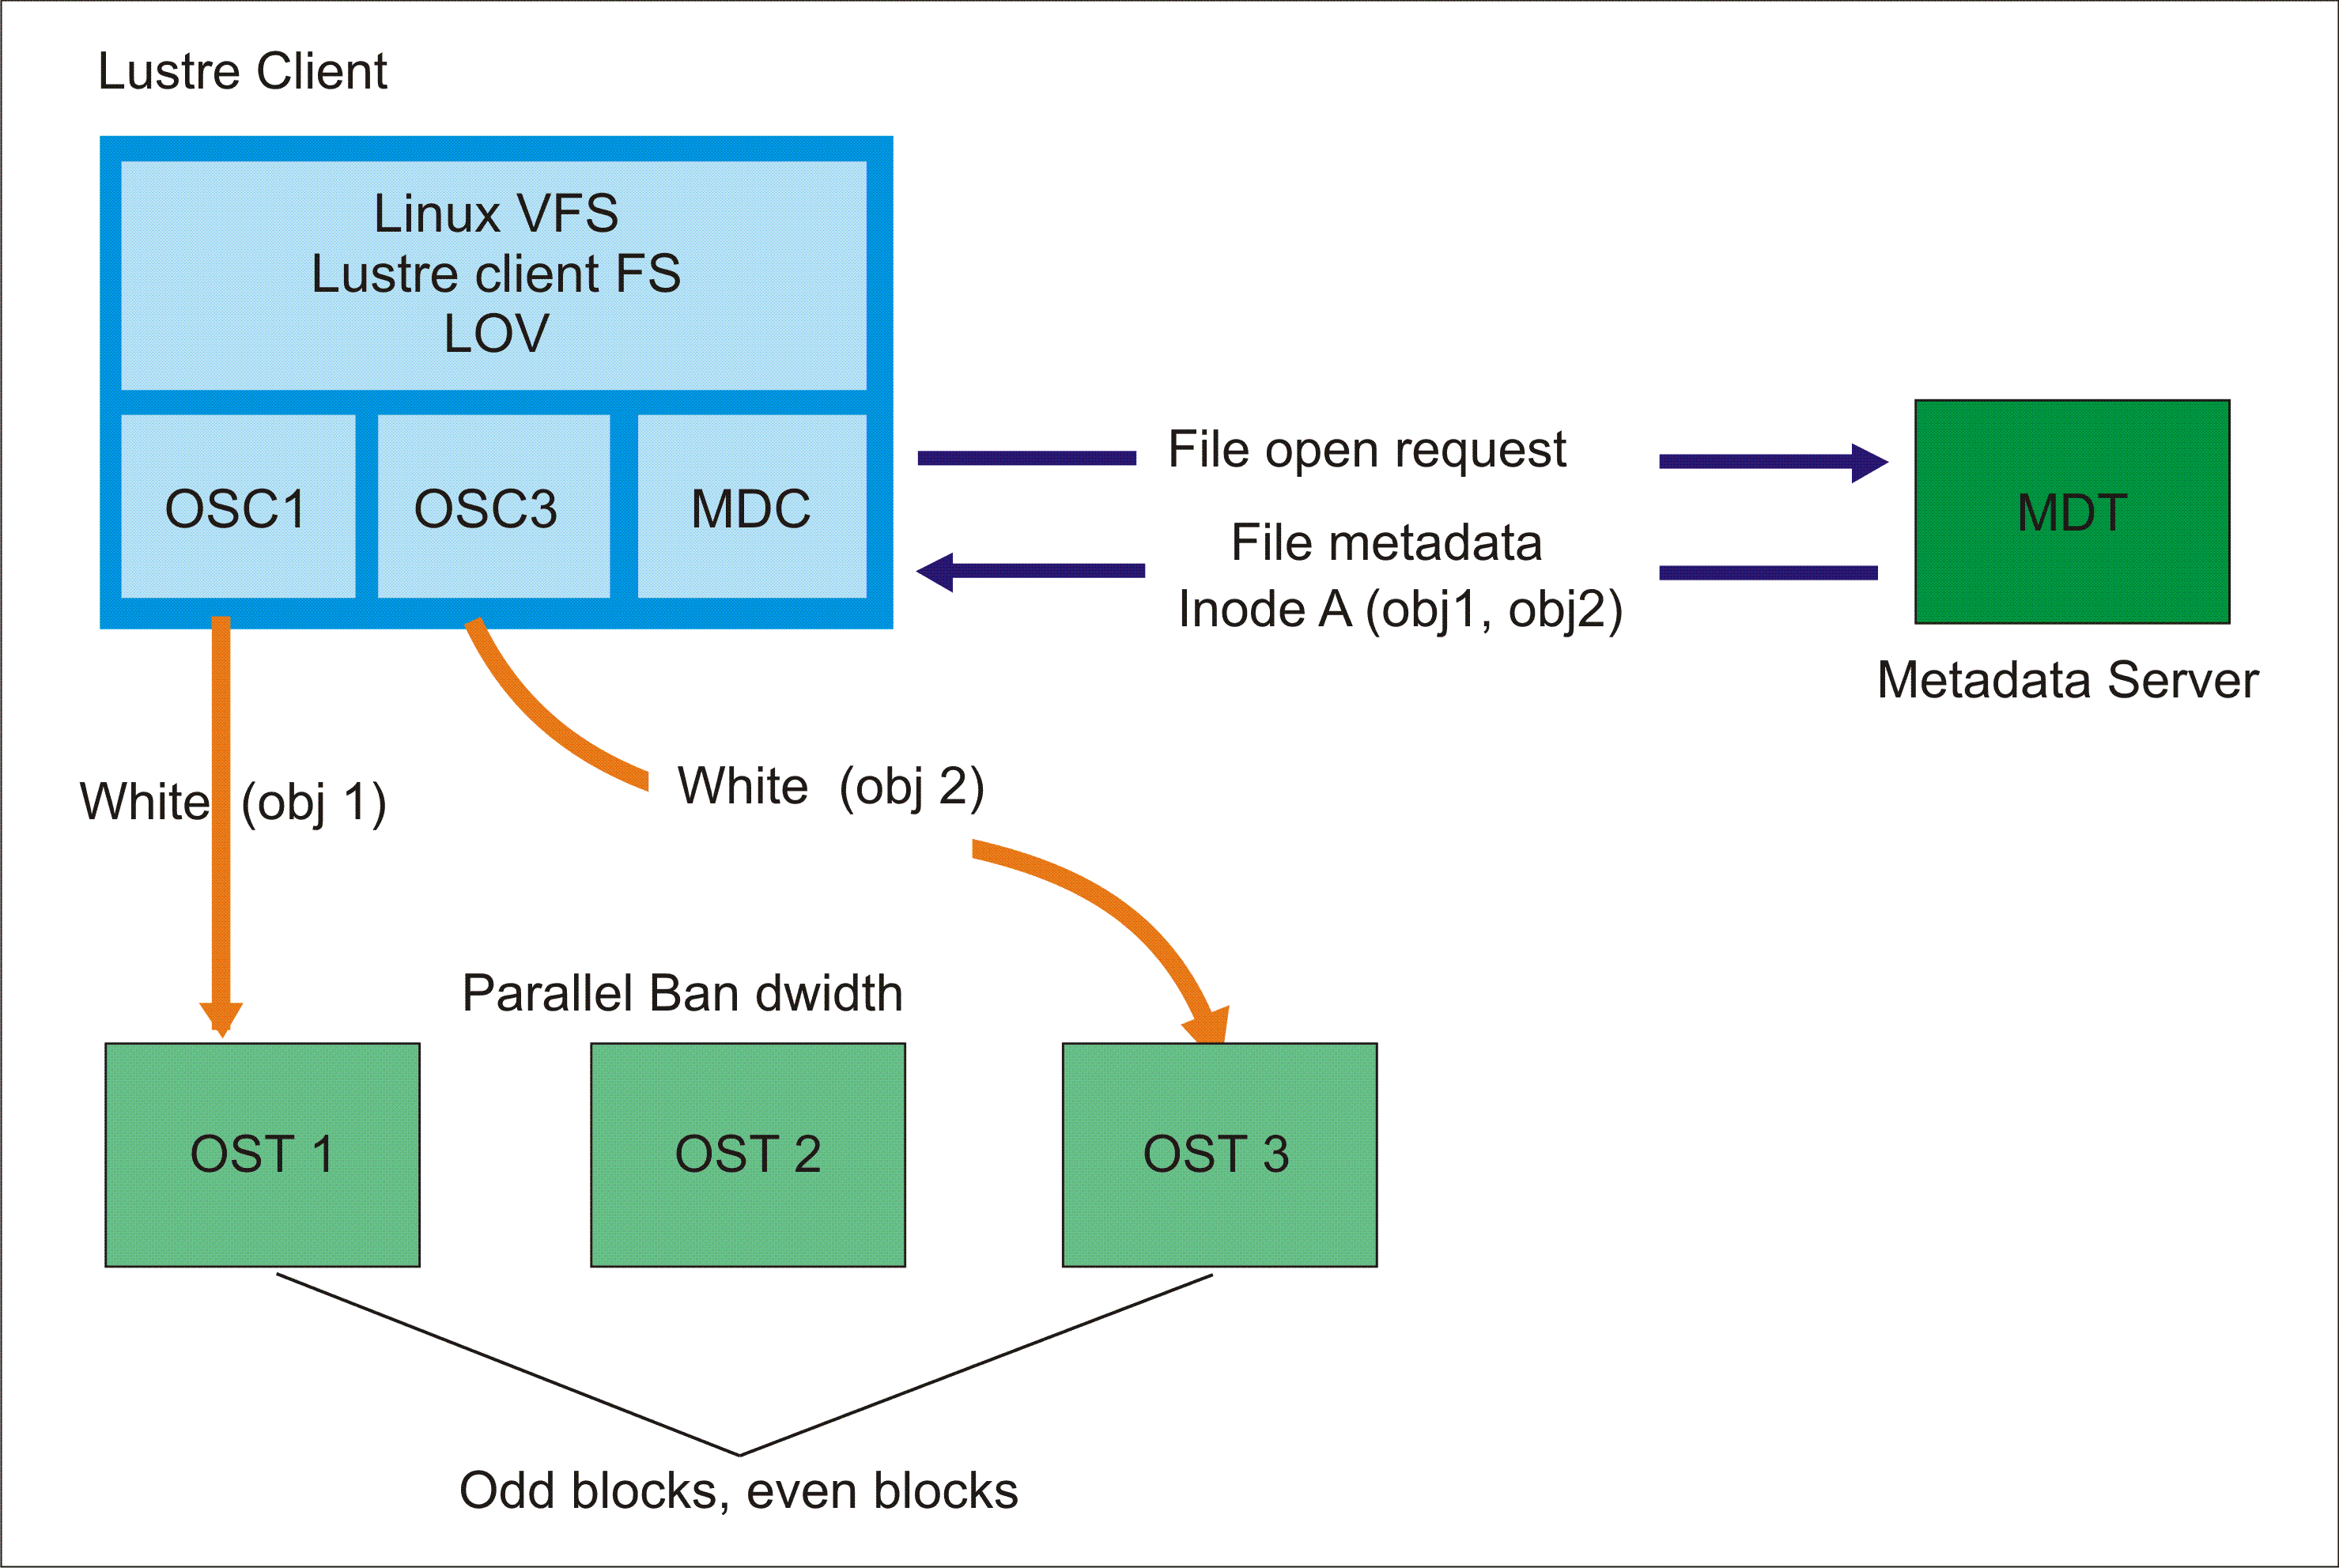
\includegraphics[width=1\textwidth]{slike/lustre_file_i_o.png}
  \caption{Lustre улазно/излазне операције}
\end{figure}

\subsection{Дељење фајлова у   \textit{Lustre}  систему}
Дељење фајлова омогућава да се делови фајлова чувају на различитим OST-има(слика 2.4). 
У RAID 0 нивоу подаци су подељени на већем броју објеката.

Број објеката се назива \textit{stripe\_count}. Сваки објекат садржи део податка. Када део податка који треба да се упише на одређени објекат прелази \textit{stripe\_count}, 
следећи део податка у датотеци се чува на следећем објекту. Дељење фајлова има  неколико предности. Једна је да максимална величина датотеке није 
ограничена величином једног OST. \textit{Lustre} може имати преко 160 подељених делова, и сваки део може да подржи максималну величину од 8TB. То доводи до максималне количине фајла од чак 1,48 PB. Још једна корист од дељења фајлова је та да је улазно/излазни пропусни опсег у једном фајлу 
збир улазно/излазних пропусних опсега за објекте од којих се фајл састоји. То у крајњем случају може бити проближно збиру пропусних опсега 160 сервера.


\begin{figure}[h!]
  \centering
      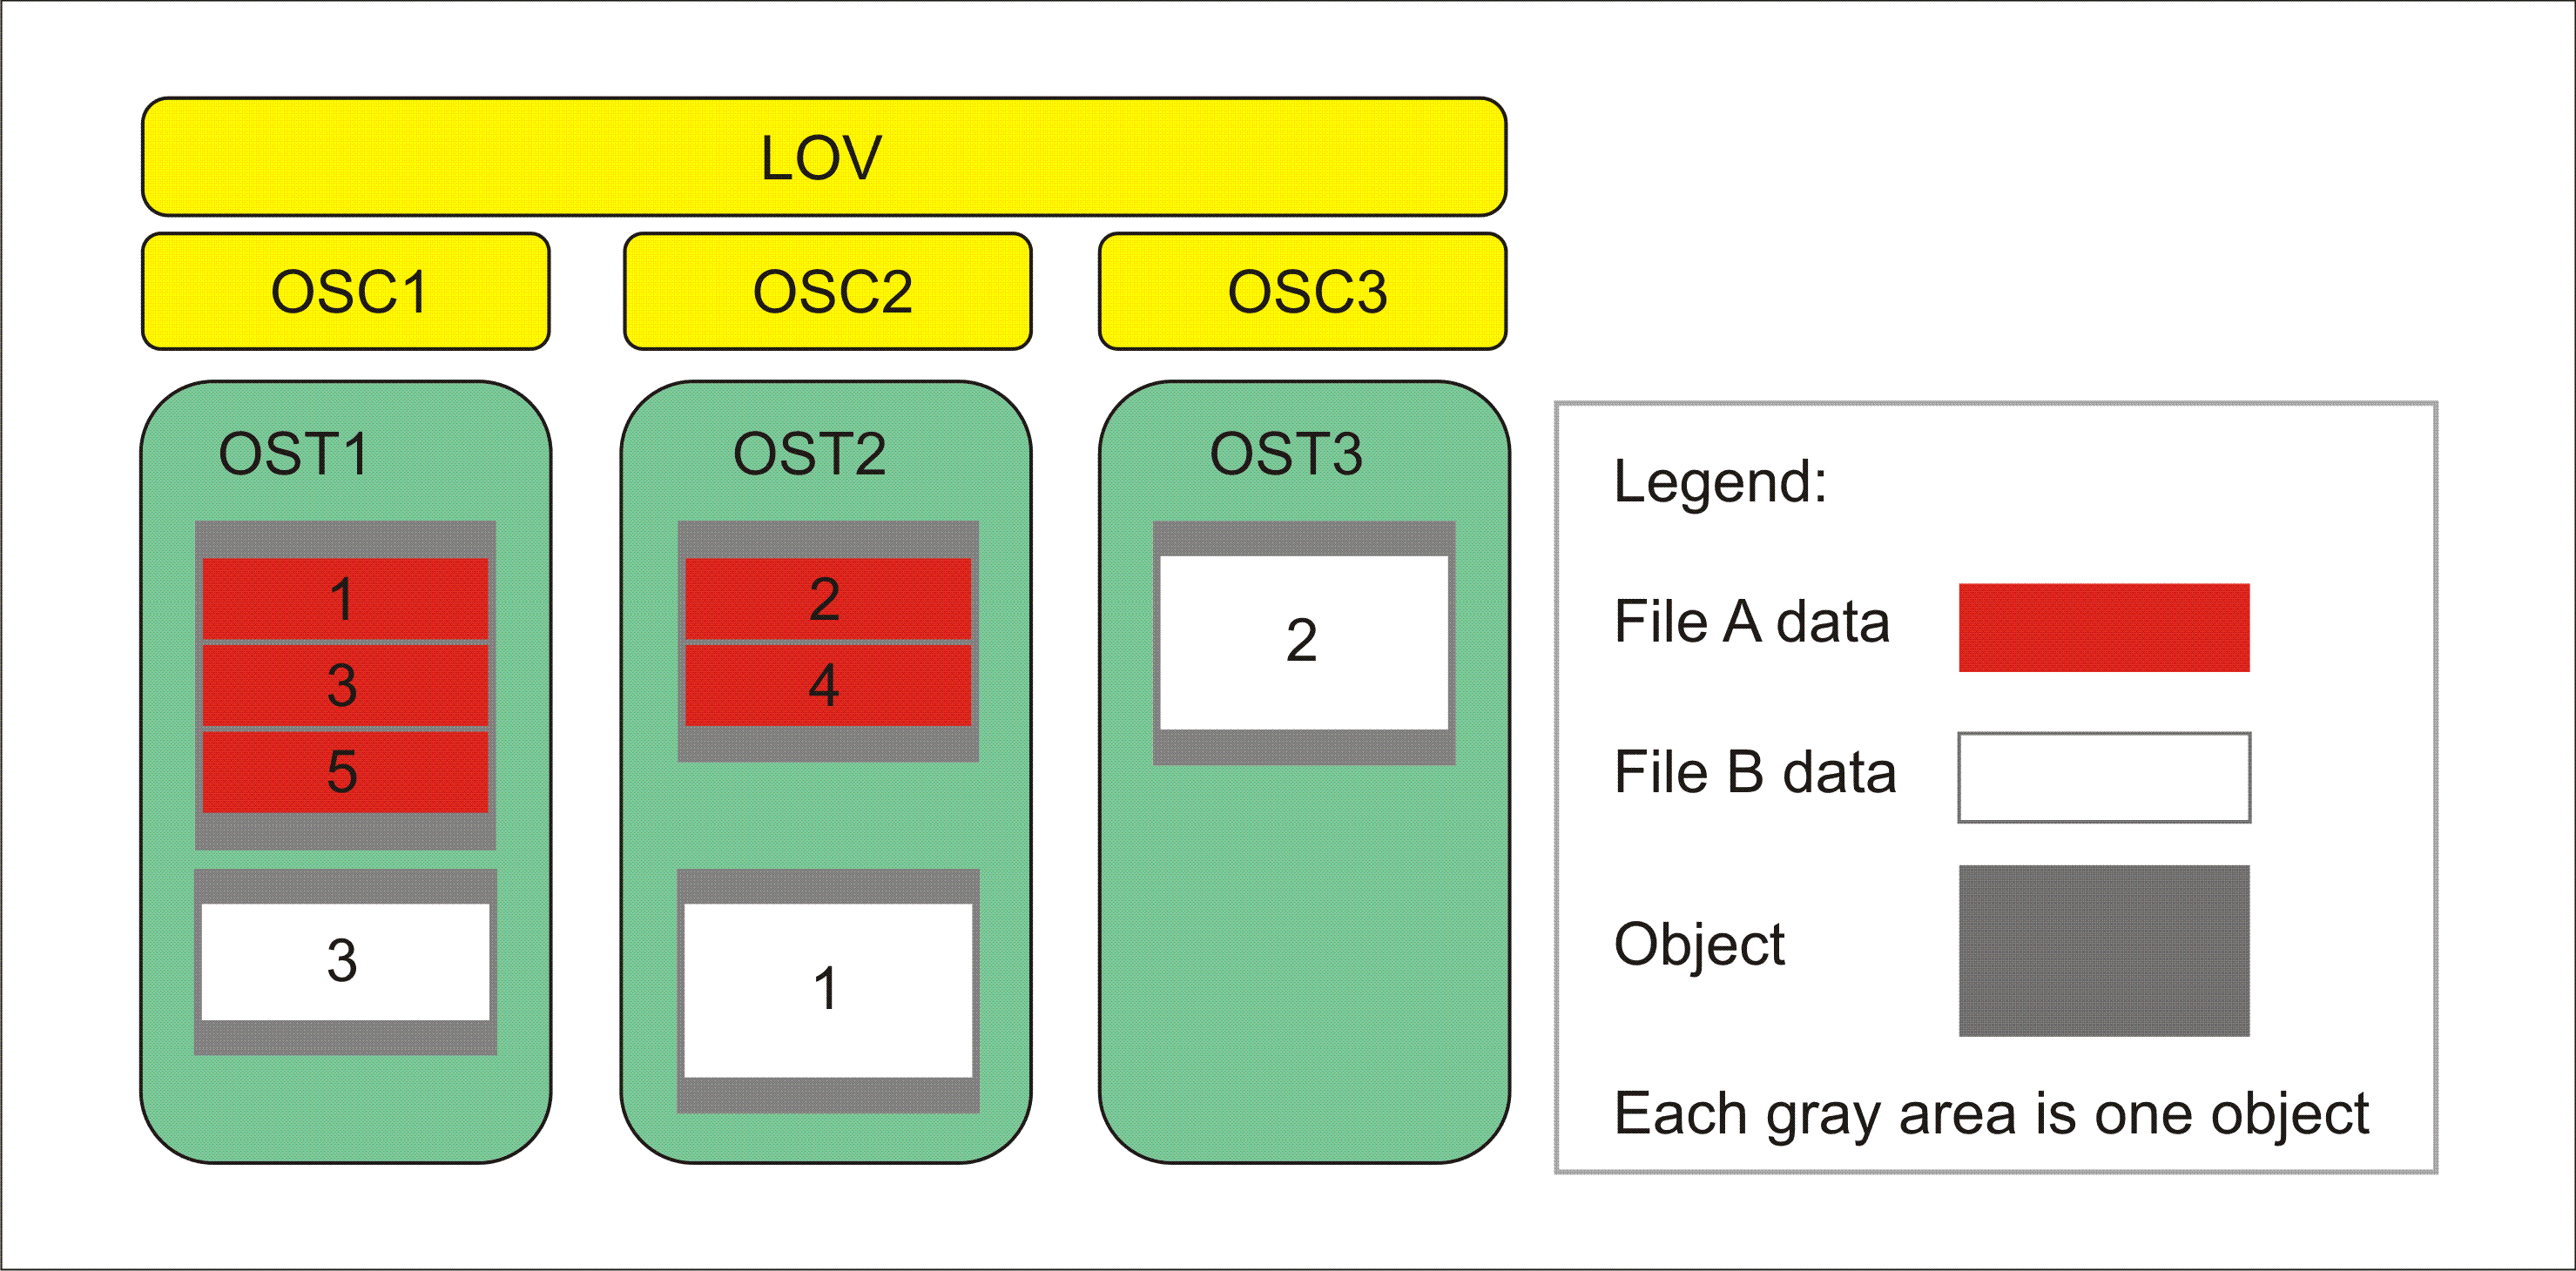
\includegraphics[width=1\textwidth]{slike/lustre_striping.png}
  \caption{Дељење фајлова}
\end{figure}

\subsection{\textit{Lustre} складиштење}
Складиштење у серверима је подељено, опционо организовано помоћу \textit{Logical
volume management (LVM)} система и форматирано као фајл систем. Lustre OSS и MDS
читају, пишу и мењају податке у формату који захтевају ови фајл системи.

\subsubsection{OSS складиштење}
Сваки OSS може управљати са више циљева за складиштење објеката (ОSТ-има), по један за сваки \textit{volume};
Улазно/излазни саобраћај је  избалансиран између ОSS-а и ОSТ-а. ОSS такође  треба да уравнотежи
пропусни опсег мреже између система мреже и складиштења и да спречи појаву уских грла. У зависности од карактеристика хардвера сервера, ОSS обично служи између 2 и 25 ОSТ-а, при чему је капацитет сваког од њих до 8 TB.

\subsubsection{MDS складиштење}
За MDS, складиштење мора бити везано за \textit{Lustre} метаподатке, за које је потребно 1-2 \% капацитета фајл система. Приступ подацима за MDS складиштење се разликује од приступа подацима за ОSS складиштења. 

\textit{Metadata} приступ подразумева рад са више захтева и читање-писање мале количине података, док улазно/излазни приступ подразумева пренос великих количина података. Велики проток података за MDS није превише битан, па се зато препоручује да се користе врсте складишта поппут FC или SAS дискова, који обезбеђују малу потражњу података. Са ниским нивоима улазно/излазних операција, RAID 5/6 није оптималан, док RAID 0+1 даје много боље резултате. \textit{Lustre} користи и \zn journaling" фајл система. За MDS се понекад могу добити и до 20 \%  бољи резултати уколико се  \zn journaling" фајл систем постави на различите дискове. Поред тога, MDS захтева велику снагу процесора и препоручује се барем четири процесорска језгра за оптималне перформансе.




\section{Kључне карактеристике}

\begin{itemize}
\item  \textbf{Скалабилност} - \textit{Lustre} перформансе зависе од броја клијентских чворова, складишта и пропусног опсега. Тренутно највећа инсталација   \textit{Lustre} система покренута у продукцији ради са 26000 клијента, на кластерима који имају између 10000-20000 клијената. Неколико   \textit{Lustre} система има капацитет од 1 PB  или више, омогућавајући складиште за 2 милијарде фајлова.

\item  \textbf{Перформансе} -   \textit{Lustre}  y продукцији има проток од око 100 GB/s. У тест окружењима перформансе су око 130 GB/s и 13,000 creates/s. 
%МИЛОШ: Објаснити ову новоуведену јединицу.
  \textit{Lustre}  клијент има проток око 2 GB/s и OSS проток од 2.5 GB/s (максимално). Такође, постоје подаци да је покренут на 240 GB/s на \textit{Spider} фајл систему у \textit{Oak Ridge National Laboratories}.

\item \textbf{\textit{POSIX} сагласност} - Потпуни \textit{POSIX} стандарди су  испуњени на   \textit{Lustre}  клијентима. Код кластера, \textit{POSIX} сагласност значи да су све операције једноставне и да клијенти увек приступају свежим подацима.

\item \textbf{Висока доступност} -   \textit{Lustre}  нуди дељено складиште OSS (за OST) и дељено складисте MDS (за MDT).

\item  \textbf{Сигурност} - У   \textit{Lustre} систему, TCP конекција се одвија само преко привилегованих портова. Припадност групама се одређује на серверу.  POSIX листе за контролу приступа (\textit{Access control lists - \gls{ACL}}) су такође подржане.

\item  \textbf{Бесплатан} -   \textit{Lustre}  је лиценциран под  GNU GPL.


\item  \textbf{Интероперативност} - \textit{Lustre} је покренут на више врста процесорских архитектура и на више верзија   \textit{Lustre} система истовремено. 

\item \textbf{Листе за контролу приступа} - Тренутно,   \textit{Lustre} безбедносни модел дозвољава UNIX фајл систем побољшан са \textit{POSIX ACLs (Access control list)}. Додатне функције укључују \textit{root squash} и конекцију само са привилегованих потрова.

\item  \textbf{Квоте} - Корисничке и групне квоте су доступне.

\item \textbf{OSS додатак} - Капацитет фајл система и проток кластера може бити повећан додавањем новог OSS са OST, и то без икаквих прекида услуге.

\item  \textbf{Контролисано дељење фајлова} - Подразумевани \textit{stripe count} и \textit{stripe size} може бити контролисан на неколико начина. Фајл систем добија стандардна подешавања приликом инсталације. Такође, директоријумима може бити додат атрибут који ће означавати начин дељења. Велики број библиотека и програма омогућавају једноставно контролисање дељења индивидуалних фајлова у   \textit{Lustre} системима.

\item  \textbf{Тренутни снимак - \textit{Snapshot}} -   \textit{Lustre}  фајл сервери користе \textit{volumes} који се налазе на серверским чворовима. У пакету   \textit{Lustre} програмa  се налази и програм који омогућава креирање  снимака свих \textit{volumes}.

\item \textbf{Алати за прављење резервних копија} -   \textit{Lustre}  подржава 2 услужна алата: Један алат скенира фајл систем и проналази измењене фајлове у датом временском периоду. Овај алат прави списак путања до измењених фајлова, а затим се ти фајлови обрађују паралелно користећи други алат. Веома  користан алат је и измењена верзија GNU tar (\textit{gtar}) која прави резервне копије и врши повратак проширених атрибута (за дељење фајла и дозволама за приступ). 
\end{itemize}


\section{Инсталација}
\subsection{Потребни   \textit{Lustre} пакети}

За инсталацију   \textit{Lustre} фајл система потребни су следећи пакети:

\begin{itemize}
\item  \textbf{\textit{Linux} кернел} закрпљен специфичним   \textit{Lustre}  закрпама (потребан само за MDS и OSS)

\item \textbf{   \textit{Lustre}  модули} компајлирани за  Linux kernel

\item   \textbf{ \textit{Lustre}  кориснички програми }потребни за конфигурацију

\item    \textbf{\textit{Lustre}  алати (\textit{e2fsck} and \textit{lfsck}) } који се користе за опоравак  фајл система, доступни у пакету под називом \textit{e2fsprogs}

\item \textbf{(Опционо) Мрежни кернел модули  и библиотеке }(на пример, кернел модули и библиотеке потребни за \textit{InfiniBand} мрежу)

\item  \textbf{\textit{e2fsprogs}}:   \textit{Lustre}  захтева сопствену верзију \textit{e2fsprogs}. \textit{e2fsprogs} мора се инсталирати само на чворовима које подижу \textit{ldiskfs} фајл системе, као што су OSS, MDS  и MGS чворови. Није потребно инсталирати их на клијентима.

\item \textbf{ \textit{\textit{Perl}}} - Разни кориснички програми за   \textit{Lustre} су писани у \textit{Perl-у}.

\end{itemize}


\subsection{Захтеви oкружења}

\begin{itemize}
\item Сви чворови   \textit{Lustre} фајл система треба да да имају \textit{remote shell} приступ. Иако није стриктно потребно за покретање система, препоручује се да сви чворови имају овакав приступ, због олакшавања конфигурације \textit{Lustre-а} и скрипти за праћење рада система. \textit{Parallel Distributed SHell (\gls{PDSH})} се препоручује, али и \textit{Secure SHell (SSH)} је прихватљив.

\item Обезбедити синхронизацију сатова. Lustre користи сатове за timestamps. Уколико сатови нису синхронизовани, доћиће до проблема код праћења рада система. Биће отежано отклањање грешака  и корелисање дневника. Препоручује се  \textit{Network Time Protocol (\gls{NTP})}.

\item Користити јединствени приступ фајловима на свим кластер чворовима. Користити исти користички ID (UID) и групни ID (GID). 

\item Искључити  \textit{Security-Enhanced Linux (\gls{SELinux})} на серверима и клијентима.   \textit{Lustre}  не подржава SELinux. Зато је потребно искључити \textit{SELinux} на свим   \textit{Lustre} чворовима, као и остале безбедносне екстензије, на пример \textit{Novell AppArmor} и \textit{network packet filtering tools (iptables)}.
\end{itemize}

\subsection{Захтеви у вези са меморијом} 

\subsubsection{Захтеви у вези са меморијом за клијенте}

Препоручљиво је да клијенти имају најмање 2 GB RAM.

\subsubsection{Захтеви у вези меморије за MDS}

Захтеви меморије за MDS зависе од следећих фактора:

\begin{itemize}

\item Броја клијента

\item Величине директоријума

\item Обима оптерећења
\end{itemize}

Количина меморије за MDS је функција броја клијената  на систему и броја фајлова које користе приликом покретања операција. То је пре свега, број закључавања клијента у једном временском тренутку. Стандардни максимум броја закључавања по чвору је 100*(број језгара), а интерактивни клијенти могу да држе више од 10000 закључавања у тренутку. За MDS, ово значи приближно 2 KB по фајлу.
Стандардно је 400 MB за  фајл систем дневника и додатна употреба меморије за кеширање фајлова за велике радне скупове који се тренутно не користе од стране клијената. Имати постојање великих података у кешу  може побољшати metadata перформансе 10x или и више ако се упоређује са читањем са диска. Приближно 1.5 KB за фајл је потребно за чување фајла у кешу. 

На пример, за MDT на MDS са  1000 клијената, 16 интерактивних  чворовима и са 2  милиона радних скупова (од којих су 400000 у кешу), потребно је 4GB меморије(Листинг 1.1)

\begin{lstlisting}[style=nonumbers,frame=single, caption=Количина меморије за MDT]
File system journal = 400 MB
1000 * 4-core clients * 100 files/core * 2kB = 800 MB

16 interactive clients * 10,000 files * 2kB = 320 MB

1,600,000 file extra working set * 1.5kB/file = 2400 MB
\end{lstlisting}

Повећање меморије аутоматски значи и боље перформансе.

Ако постоје директоријуми који садрже милион или више фајлова, можда ће бити потребно значајно  више меморије. На пример, у окружењу где клијенти насумично приступају једном од 10 милиона фајлова, постоји и додатна меморија за кеш.

\subsubsection{Захтеви у вези са меморијом за OSS}

 
Приликом планирања хардвера за OSS чвор, треба размотрити употребу меморије у   \textit{Lustre} систему (нпр. дневник, сервисне нити, фајл систем метаподатака, итд.). Такође, треба размислити колико је битно да OSS  кешира податке.

 
\begin{itemize}
\item \textbf{Величина дневника} - Стандардно, сваки   \textit{Lustre} \textit{ldiskfs} фајл систем има 400 MB за дневник. Ово може бити једнако количини меморије на  OSS чвору по једном фајл систему.

\item \textbf{Сервисне нити} - Нити на OSS чвору алоцирају око 1 MB за улазно/излазни бафер за сваку OST сервисну нит, тако да ове бафере није потребно алоцирати за сваки улазно/излазни захтев.

\item \textbf{Метаподаци фајл система} - Разумна количина меморије би требало да буде доступна за фајл систем метаподатака. Уколико је меморија доступна, онда се улазно/излазне операције на диску одвијају брже.

\item \textbf{Мрежни транспорт} - Уколико се користи  TCP или неки други протокол, треба да се има у виду меморија за бафере за слање/пријем.

\item \textbf{Конфигурација у случају отказа} - Ако се OSS чвор користи за \textit{failover} са другог чвора, онда RAM меморија за сваки дневник треба бити дуплирана тако да сервер за резервне копије може да реши проблем уколико матични сервер откаже.

\item \textbf{OSS читање кеша} - омогућава само читање кешираних података на OSS, користећи регуларану \textit{Linux} кеш страну за чување података. Исто као кеширање са регуларног фајл система на \textit{Linux} оперативном систему, OSS чита кеш користећи што више физичке меморије.
\end{itemize}

\subsubsection{Израчунавање количине меморије за  OSS }

Минимална препоручена количина RAM меморије OSS-а са 2 OST-а је 4 GB(Листинг 1.2).


\begin{lstlisting}[style=nonumbers,frame=single, caption=Препоручена количина RAM меморије]
1.5 MB per OST IO thread * 512 threads = 768 MB

e1000 RX descriptors, RxDescriptors=4096 for 9000 byte MTU = 128 MB

Operating system overhead = 512 MB

400 MB journal size * 2 OST devices = 800 MB

600 MB file system metadata cache * 2 OSTs = 1200 MB
\end{lstlisting}

1700 MB је за алокацију бафера и додатна 2GB за минималан фајл систем и кернел. Значи за стандардну конфигурацију минимум  меморије је 4 GB за сваки OSS чвор са 2 OST. Иако то није стриктно речено додавањем више меморије на OSS долази до побољшања перформансе читања мањих често посећиваних фајлова. 
За \textit{failover} конфигурацију, минимална количина RAM меморије је 6 GB. За 4 OST-а на сваком OSS-у, у \textit{failover} конфигурацији потребно је 10GB.

\section{Инсталација   \textit{Lustre} фајл система}
\subsection{Инсталација оперативног система}

Да би се инсталирао \textit{Lustre} фајл систем, потребно је имати најмање 3, а пожељно је имати 4 чвора. 

За ову инсталацију користи се \textit{Xubuntu} 14.04 оперативни систем на којем је инсталираn \textit{VirtualBox} 4.3.10, помоћу којег се креирају 4 виртуалне машине(Слика 1.5). Свакој машини је potrebno додеliti 768MB RAM меморије и 1 процесор.
\begin{figure}[h!]
  \centering
      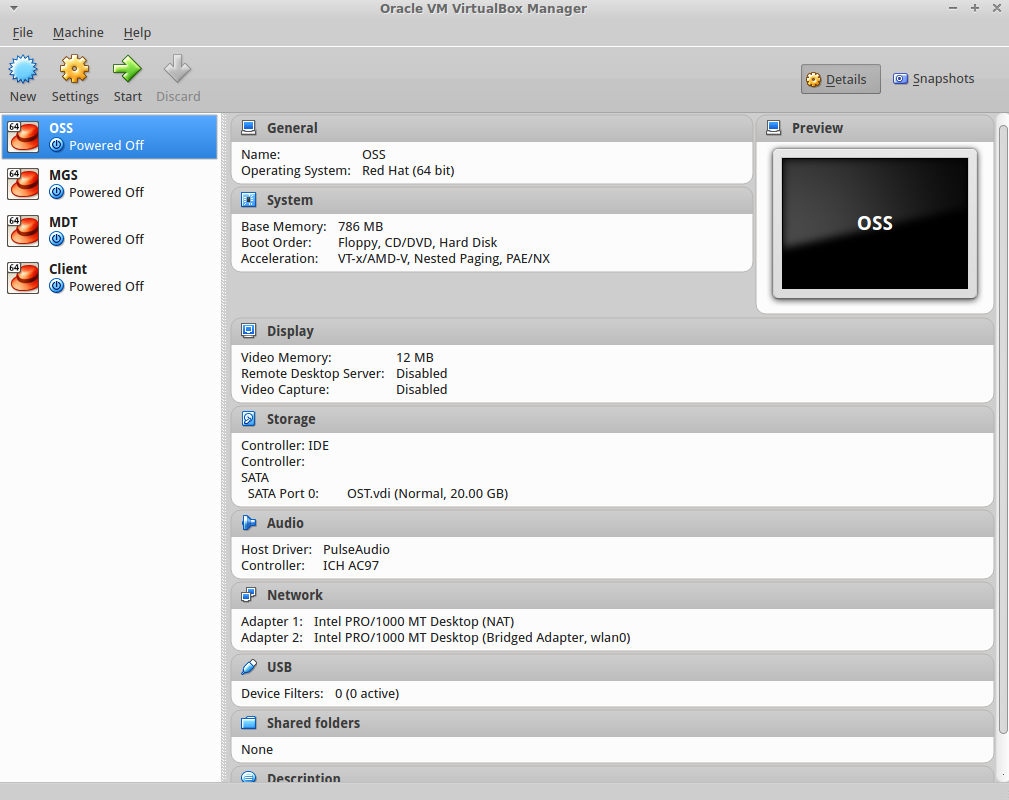
\includegraphics[width=1\textwidth]{slike/virtualbox.png}
  \caption{Bиртуалне машине}
\end{figure}
Да би машина имала приступ интернету, потребно је у подешавањима, у секцији \textit{Network} поставити први адаптер на \gls{NAT}, a други на \textit{Bridged Adapter}. 	\textit{Bridged Adapter} је потребан да би машине комуницирале у локалној мрежи.
~\\[3cm]
На свим чворовима биће инсталиран \textit{Scientific Linux 6.5} и сваком чвору бити додељена по једна статичка IP адреса(Табела 1.1).
\begin{center}
\captionof{table}{Тестна конфигурација   \textit{Lustre} чворова}
    \begin{tabular}{ | l | l | l | p{5cm} |}
    \hline
    \textbf{Оперативни систем} & \textbf{Назив} & \textbf{IP } & \textbf{Функција} \\ \hline
Scientific Linux 6.5 & mgs &  192.168.1.200 & Managment Server \\ \hline
Scientific Linux 6.5 & mdt &  192.168.1.201 & Metadata Server \\ \hline
Scientific Linux 6.5 & oss &  192.168.1.202 & OS Server \\ \hline
Scientific Linux 6.5 & client &  192.168.1.203 & Client \\ \hline
    \end{tabular}

\end{center}

На MGS-у, MDT-у и OSS-у чврсти диск је подељен на:
\begin{itemize}
\item \textit{Boot} партиција – 10 GB (\textit{root}, \textit{home} директоријум)

\item \textit{Swap} партиција – 2 GB

\item Logical volume partition – 8 GB ( \gls{LVM} партиција за   \textit{Lustre} фајл систем)
\end{itemize}


Након инсталације оиперативног система, потребно је урадити следеће кораке:

\begin{enumerate}
\item  Обезбедити SSH приступ између свих машина. 
SSH daemon се стартује командом
\begin{verbatim}
/etc/init.d/sshd start
\end{verbatim}
док следећом командом подешавамо да се  SSH сервис покреће приликом подизања оперативног система
\begin{verbatim}
chkconfig sshd on
\end{verbatim}

\item Инсталација потребних програма

Да бисмо касније компајлирали кернел, потребни су пакети попут \textit{gcc, make} ... Њих инсталирамо командом:

\begin{verbatim}
yum -y groupinstall "Development Tools"
\end{verbatim}

\item Додавање  IP адреса у \textit{/etc/hosts} фајл. На свим чворовима додати следеће линије у \textit{/etc/hosts} фајл:
\begin{verbatim}
192.168.1.200   mgs
192.168.1.201   mdt
192.168.1.202   ost
192.168.1.203   client
\end{verbatim}

\item  Искључити  \textit{Linux Firewall}
\begin{verbatim}
chkconfig iptables off
\end{verbatim}

\item Потребно је скинути    \textit{Lustre} пакете(Листинг 1.3).
\begin{lstlisting}[style=nonumbers,frame=single, caption= \textit{Lustre} пакетi]
cd  /home/mgs/Downloads/

wget http://downloads.whamcloud.com/public/lustre/latest-maintenance-release/el6/server/RPMS/x86_64/
kernel-2.6.32-358.23.2.el6_lustre.x86_64.rpm

wget http://downloads.whamcloud.com/public/lustre/latest-maintenance-release/el6/server/RPMS/x86_64/
kernel-firmware-2.6.32-358.23.2.el6_lustre.x86_64.rpm

wget http://downloads.whamcloud.com/public/lustre/latest-maintenance-release/el6/server/RPMS/x86_64/
lustre-2.4.2-2.6.32_358.23.2.el6_lustre.x86_64.x86_64.rpm

wget http://downloads.whamcloud.com/public/lustre/latest-maintenance-release/el6/server/RPMS/x86_64/
lustre-ldiskfs-4.1.0-2.6.32_358.23.2.el6_lustre.x86_64.x86_64.rpm

wget http://downloads.whamcloud.com/public/lustre/latest-maintenance-release/el6/server/RPMS/x86_64/
lustre-modules-2.4.2-2.6.32_358.23.2.el6_lustre.x86_64.x86_64.rpm

wget http://downloads.whamcloud.com/public/lustre/latest-maintenance-release/el6/server/RPMS/x86_64/
lustre-osd-ldiskfs-2.4.2-2.6.32_358.23.2.el6_lustre.x86_64.x86_64.rpm

wget http://downloads.whamcloud.com/public/e2fsprogs/latest/el6/RPMS/i686/e2fsprogs-1.42.7.wc2-7.el6.i686.rpm

wget http://downloads.whamcloud.com/public/e2fsprogs/latest/el6/RPMS/i686/e2fsprogs-libs-1.42.7.wc2-7.el6.i686.rpm

wget http://downloads.whamcloud.com/public/e2fsprogs/latest/el6/RPMS/i686/libss-1.42.7.wc2-7.el6.i686.rpm

wget http://downloads.whamcloud.com/public/e2fsprogs/latest/el6/RPMS/i686/libcom_err-1.42.7.wc2-7.el6.i686.rpm
\end{lstlisting}

\item Ископирати пакете на OSS i MDT помоћу команде \texttt{scp}:
\begin{verbatim}
scp -r /home/mgs/Downloads/ ost:/home/ost/
scp -r /home/mgs/Downloads/ mdt:/home/mdt/
\end{verbatim}

\item Креирати фајл \textit{/etc/modprobe.d/lustre.conf} и подесити мрежни протокол и мрежно окружење додавањем следеће линије:
\begin{verbatim}
	options lnet networks=tcp0(eth1)
\end{verbatim}

\item Такоће, ископирати \textit{lustre.conf} на OSS i MDT:
\begin{verbatim}
scp  /etc/modprobe.d/lustre.conf mdt:/etc/modprobe.d/lustre.conf
scp  /etc/modprobe.d/lustre.conf ost:/etc/modprobe.d/lustre.conf
\end{verbatim}

% MИЛОШ: Зашто овде кажеш да се кернел компајлира??? Исправио сам у "инсталирати".
\item Инсталирати \textit{Lustre} кернел:
\begin{lstlisting}[style=nonumbers,frame=single, caption=Инсталација \textit{Lustre} кернела]
rpm -ivh kernel-2.6.32-358.23.2.el6_lustre.x86_64.rpm  kernel-firmware-2.6.32-358.23.2.el6_lustre.x86_64.rpm 
\end{lstlisting}
\item Инсталирати \textit{e2fsprogs} 
\textit{e2fsprogs} је скуп програма за одржавање \textit{Linux} фајл система. \textit{e2fsprogs} садржи неколико програма од којих су најпознатији:

\begin{itemize}
\item \textbf{\textit{e2fsck}} - Проверава и поправља несугласице.
\item \textbf{\textit{mke2fs}} - Креирa ext2, ext3 и ext4 фајл системe.
\item \textbf{\textit{resize2fs}} - Промена величине фајл система.
\item \textbf{\textit{tune2fs}} - Подешавање параметара фајл система.
\item \textbf{\textit{logsave}} - Снимање логова.
\item \textbf{\textit{e2label}} - Променa лабеле фајл система.
\item \textbf{\textit{findfs}} - Претрагa фајл система по лабели или UUID.
\item \textbf{\textit{badblocks}} - Претрагa лоших сектора.
\item \textbf{\textit{blkid}} - Штампа атрибутe блокова.
\item \textbf{\textit{chattr}}  - Променa атрибута фајлова.
\end{itemize}

Инсталирати \textit{e2fsprogs} (Листинг 1.5).

\begin{lstlisting}[style=nonumbers,frame=single,caption=Инсталација \textit{e2fsprogs}]
rpm -Uvh e2fsprogs-1.42.7.wc2-7.el6.x86_64.rpm  e2fsprogs-libs-1.42.7.wc2-7.el6.x86_64.rpm libcom_err-1.42.7.wc2-7.el6.x86_64.rpm libss-1.42.7.wc2-7.el6.x86_64.rpm 
\end{lstlisting}

\item  Инсталирати   \textit{Lustre} кернел модула(Листинг 1.6).

\begin{lstlisting}[style=nonumbers,frame=single,caption=Инсталација кернел модула]
rpm -ivh lustre-modules-2.4.2-2.6.32_358.23.2.el6_lustre.x86_64.x86_64.rpm lustre-ldiskfs-4.1.0-2.6.32_358.23.2.el6_lustre.x86_64.x86_64.rpm
\end{lstlisting}

\item Инсталација   \textit{Lustre} фајл система 
Како би се   \textit{Lustre} лакше надгледао, потребно је инсталирати \textit{net-snmp-libs (Simple Network Management Protocol (\gls{SNMP}) )} (Листинг 1.7). SNMP је протокол за надгледање мрежне опреме. Net-SNMP је пакет апликација које се користе за имплементацију SNMP користећи IPv4, као и IPv6.

\begin{lstlisting}[style=nonumbers,frame=single,caption= Инсталација Net-SNMP-а]
yum install net-snmp-libs

rpm -ivh lustre-osd-ldiskfs-2.4.2-2.6.32_358.23.2.el6_
lustre.x86_64.x86_64.rpm

rpm -ivh lustre-2.4.2-2.6.32_358.23.2.el6_lustre.x86_64.x86_64.rpm
\end{lstlisting}


\item Искључивање \textit{SELinux}-а 
Да би се   \textit{Lustre} покренуо потребно је искључити \textit{Security-Enhanced Linux (SELinux)} (Листинг 1.8). \textit{SELinux} је безбедоносни кернел модул.
У фајл \textit{/boot/grub/grub.conf} додати selinux=0.

\begin{lstlisting}[style=nonumbers,frame=single,caption= Команде за искључивање \textit{SELinux}-а]

kernel /boot/vmlinuz-2.6.32-358.23.2.el6\_lustre.x86\_64 ro root=UUID=2c8a0af6-545a-4761-9e41-74cfe026385e 
rd\_NO\_LUKS rd\_NO\_LVM LANG=en\_US.UTF-8 rd\_NO\_MD SYSFONT=latarcyrheb-sun16 crashkernel=auto  KEYBOARDTYPE=pc
 KEYTABLE=us rd\_NO\_DM rhgb quiet selinux=0

reboot 
\end{lstlisting}

\item Креирати физичких \textit{volumes} за LVM систем на МGS, MDT, OSS(Листинг 1.9).
\begin{lstlisting}[style=nonumbers,frame=single, caption=Излаз команде \textit{fdisk -l}]
fdisk -l

/dev/sda1   *           1        1306    10485760   83  Linux
/dev/sda2            1306        2350     8387584   83  Linux
/dev/sda3            2350        2611     2097152   82  Linux swap/Solaris
\end{lstlisting}

\begin{verbatim}
pvcreate /dev/sda2
\end{verbatim}

Команда \textit{pvs} даје излаз приказан на Листингу 1.10.

\begin{lstlisting}[style=nonumbers,frame=single], caption=Излаз команде \textit{pvs}]
  PV         VG   Fmt  Attr PSize PFree
  /dev/sda2       lvm2 a--  8.00g 8.00g
\end{lstlisting}

\item Креирати групу \textit{volumes}

\begin{verbatim}
vgcreate lustre /dev/sda2
\end{verbatim}

Команда \textit{vgs} даје следећи приказан на Листингу 1.11.

\begin{lstlisting}[style=nonumbers,frame=single, caption=Излаз команде \textit{vgs}]
  VG     #PV #LV #SN Attr   VSize VFree 
  lustre   1   1   0 wz--n- 8.00g 8.00g
\end{lstlisting}

У зависности од типа сервисног чвора покренути команду и креирати логичке \textit{volumes}(Листинг 1.12).

\begin{lstlisting}[style=nonumbers,frame=single, caption=Креирање логичких \textit{volumes}]
lvcreate -L 7.9G -n MGS lustre
lvcreate -L 7.9G -n MDT lustre
lvcreate -L 7.9G -n OST lustre
\end{lstlisting}

% МИЛОШ: Смањи фонт за ове lstlistings у темплејту, како би што више могло да стане у један ред

\item Конфигурисати MGS

Креирати MGS фајл систем, а затим га и подигнути(Листинг 1.13).
\begin{lstlisting}[style=nonumbers,frame=single, caption=Креирање MGS фајл систем]
mkfs.lustre --mgs /dev/lustre/MGS
mkdir -p /mnt/MGS/
mount -t lustre /dev/lustre/MGS /mnt/MGS/ 
\end{lstlisting}


Команда  \textit{df} даје следећи излаз приказан на Листингу 1.14.
\begin{lstlisting}[style=nonumbers,frame=single, caption= Излаз \textit{df} команде]
Filesystem           1K-blocks      Used Available Use% Mounted on
/dev/sda1             10321208   2615424   7600960  26% /
tmpfs                   388408        72    388336   1% /dev/shm
/dev/mapper/lustre-MGS
                       8156088    347176   7394604   5% /mnt/MGS
\end{lstlisting}


\item Конфигурисати MDT 
Креирати MDT фајл систем, а затим га и подигнути(Листинг 1.15).

\begin{lstlisting}[style=nonumbers,frame=single, caption=Креирање MDT фајл систем]
mkfs.lustre --fsname=lustre --mdt  --mgsnode=mgs@tcp0 /dev/lustre/MDT 
mkdir -p /mnt/MDT/
mount -t lustre /dev/lustre/MDT /mnt/MDT/ 
\end{lstlisting}


\item Конфигурисати OSS 
Креирати OSS фајл систем, а затим га и подигнути(Листинг 1.16).
\begin{lstlisting}[style=nonumbers,frame=single, caption=Креирање OSS фајл систем]
mkfs.lustre --fsname=lustre --ost  --index=1 --mgsnode=mgs@tcp0 /dev/lustre/OST 
mkdir -p /mnt/OST/
mount -t lustre /dev/lustre/OST /mnt/OST/ 
\end{lstlisting}


\item Конфигурисати клијента 
На клијенту је потребно инсталирати \textit{Lustre} клијент пакете(Листинг 1.17). 
\begin{lstlisting}[style=nonumbers,frame=single, caption= Команде за инсталацију \textit{Lustre} клијент пакета]
yum -y groupinstall "Development Tools"

yum install net-snmp-libs

wget http://downloads.whamcloud.com/public/lustre/latest-maintenance-release/el6/client/RPMS/x86\_64/
lustre-client-modules-2.4.2-2.6.32\_358.23.2.el6.x86\_64.x86\_64.rpm

http://downloads.whamcloud.com/public/lustre/latest-maintenance-release/el6/client/RPMS/x86\_64/
lustre-client-2.4.2-2.6.32\_358.23.2.el6.x86\_64.x86\_64.rpm

yum localinstall  lustre-client-2.4.2-2.6.32\_358.23.2.el6.x86\_64.x86\_64.rpm 
lustre-client-modules-2.4.2-2.6.32\_358.23.2.el6.x86\_64.x86\_64.rpm 

mkdir /lustre

reboot
\end{lstlisting}


Подизање   \textit{Lustre} фајл система врши се командом:
\begin{verbatim}
mount -t lustre mgs@tcp0:/lustre /lustre
\end{verbatim}

Уколико је све конфигурисано као што је назначено, команда  \textit{df} треба да да следећи излаз приказан на Листингу 1.18.
\begin{lstlisting}[style=nonumbers,frame=single, caption= Излаз команде \textit{df}]

Filesystem           1K-blocks      Used Available Use% Mounted on
/dev/sda1             18577148   2735112  15653360  15% /
tmpfs                   388408        72    388336   1% /dev/shm
mgs@tcp0:/lustre       8156088    365396   7376384   5% /lustre

\end{lstlisting}

\end{enumerate}



\section{Кориснички алати за подешавање система}
\subsection{Алати за откривање грешака} 
  \textit{Lustre}  је сложен систем и може се наићи на разнолике проблеме при коришћењу. Треба имати алат за откривање грешака при руци, који може помоћи у схватању проблема и разлога његовог настанка. Разноврсни алати за дијагностику и анализе су доступни приликом отклањања проблема са   \textit{Lustre}  софтвером. Неки од њих се налазе у \textit{Linux} дистрибуцијама, док су
други  развијени и доступни су у оквиру    \textit{Lustre} пројекта. Следећи  \textit{in-kernel} механизми за отклањање грешака  су уграђени у   \textit{Lustre}  софтвер:

\begin{itemize}
\item  \textit{Debug logs}

\item  \textit{Debug} позадински сервис

\item  \textit{/proc/sys/lnet/debug}
\end{itemize}
Следећи програми су такође укључени у   \textit{Lustre} :
\begin{itemize}
\item \textit{lctl}

\item   \textit{Lustre subsystem asserts}

\item \textit{lfs}
\end{itemize}
Поред њих, ту су и општи алати који су уграђени у стандардне \textit{Linux} дистрибуције:
\begin{itemize}
\item \textit{strace}

\item \textit{/var/log/messages}

\item \textit{Crash dumps}

\item debugfs
\end{itemize}
Следећи \textit{logging} алати могу се користити за скупљање информација приликом откривања   \textit{Lustre}  \textit{kernel} проблема.
\begin{itemize}
\item \textit{kdump}

\item \textit{netconsole}

\item \textit{netdump}
\end{itemize}

За отклањање грешака   \textit{Lustre}  система у развојном окружењу користи се \textit{leak\_finder.pl}, док се за отклањање грешака и анализу користе
\begin{itemize}
\item \textit{kgdb}
\item \textit{crash}.
\end{itemize}

% МИЛОШ: Овде опет фали неки везивни текст. 
Кориснички програми:
\begin{itemize}
\item \textit{mkfs.lustre}
\item \textit{tunefs.lustre}
\item \textit{lctl}
\item \textit{mount.lustre}
\item \textit{lustre\_rsync}
\item Додатни кориснички програми за подешавање конфигурације
\end{itemize}

\subsection{mkfs.lustre}
\textit{mkfs.lustre} je кориснички програм који форматира диск за   \textit{Lustre} фајл систем.

Синтакса ове команде је:
\begin{verbatim}
mkfs.lustre <target_type> [options] device
\end{verbatim}
где је \textit{<target\_type>} један од следећих типова:

\begin{itemize}
\item \textbf{--ost}
\textit{Object Storage Target (OST)}
\item \textbf{--mdt}
\textit{ Metadata Storage Target (MDT)}
\item \textbf{--network=net }
врста мреже којом су повезани OST и MDT
\item \textbf{--mgs }
\textit{ Configuration Management Service (MGS)} може бити комбинован са  --mdt
\end{itemize}
После форматирања диска, диск може бити коришћен од стране   \textit{Lustre} сервиса.
Када је диск креиран, истом командом се  могу подесити параметри  одговарајућег диска.
Параметри се додају као \textit{--param} опција \textit{mkfs.lustre} команде.

Параметри \texttt{mkfs.lustre} команде су:

\begin{itemize}
\item \textbf{\textit{--backfstype=fstype }}
Поставља посебан формат за резервне копије фајл система (као што су \textit{ext3}, \textit{ldiskfs}).
\item \textbf{\textit{ --comment }}
Поставља кориснички коментар.
\item \textbf{\textit{--device-size=KB }}
Поставља величину уређаја.
\item \textbf{\textit{--dryrun }}
Штампа шта ће бити учињено. Не утиче на операције са диском.
\item \textbf{\textit{--failnode=nid }}
Поставља Ид партнера за отказе.
\item \textbf{\textit{--fsname=filesystem\_name }}
Поставља назив   \textit{Lustre} фајл система којег ће бити део. Подразумевани је \zn lustre”. Назив може имати највише 8 карактера.
\item \textbf{\textit{--index=index }}
Поставља OST или MDT индекс.
\item \textbf{\textit{--mkfsoptions=opts }}
Поставља опције за резервне копије.  Опције могу бити постављене овде су ext3.
\item \textbf{\textit{--mountfsoptions=opts} }
Поставља опције које се користе приликом монтирања диска.
\item \textbf{\textit{--mgsnode=nid }}
Постављају NID за MGS чвор.
\item \textbf{\textit{--param sys.timeout=40 }}
Поставља тајм-аут система.
\item \textbf{ \textit{--param lov.stripesize=2M }}
Поставља stripe количину меморије.
\item \textbf{\textit{--param lov.stripecount=2 }}
Поставља број stripe делова.
\item \textbf{\textit{--param failover.mode=failout }}
Враћа грешке диска, уместо да чека на опоравак.
\item \textbf{\textit{--reformat }}
Реформатира диск.

\end{itemize}

\subsection{\textit{tunefs.lustre}}

Кориснички програм који мења конфигурацију на   \textit{Lustre} диску је \textit{tunefs.lustre}.
Синтакса ове команде је:
\begin{verbatim}
tunefs.lustre [options] device
\end{verbatim}

Овом командом се може инсталирати најновија верзија   \textit{Lustre} система, с тим што се приликом извршавања ове команде не брише садржај диска. Измене после извршавања команде се могу уочити након следећег подизања диска.

\textit{tunefs.lustre} поставља параметре додавањем нових или мењањем старих. За брисање старих параметара и додавање нових потребно је покренути:
\begin{verbatim}
 tunefs.lustre --erase-params --param=<new parameters>
 \end{verbatim}
Параметри \textit{tunefs.lustre} команде су:
\begin{itemize}

\item \textbf{\textit{--comment=comment }}
Поставља кориснички коментар.
\item \textbf{\textit{--dryrun}} 
Штампа шта ће бити учињено. Не утиче на операције са диском.
\item \textbf{\textit{--erase-params} }
Брише све претходне параметре.
\item \textbf{\textit{--failnode=nid} }
Поставља Ид партнера за отказе
\item \textbf{\textit{--fsname=filesystem\_name }}
Поставља назив   \textit{Lustre}  фајл система којег ће бити део. Подразумевани је \zn \textit{lustre}”.
\item \textbf{\textit{--index=index }}
Поставља OST или MDT индекс.

\item \textbf{\textit{--mkfsoptions=opts }}
Поставља опције за резервне копије. Опције које могу бити постављене овде су ext3.
\item \textbf{\textit{--network=net }}
Поставља мрежу преко које су повезани OST/MDT чворови.
\item \textbf{\textit{--mgs }}
Додаје сервис за управљање конфигурацијом.
\item \textbf{\textit{--msgnode=nid,... }}
Поставља  NID(s) за MGS чвор
\item \textbf{\textit{--nomgs} }
Уклања сервис за управљање конфигурацијом.
\item \textbf{\textit{--quiet }}
Штампа основних информације.

\item \textbf{\textit{--verbose }}

Штампа више информације.
\item \textbf{\textit{--writeconf }}
Брише све конфигурационе дневнике за фајл систем на коме је MDT, а затим их регенерише. Приликом извршавања ове команде може доћи до престанка рада сервера и клијената. У општем случају, ова команда треба да буде извршена само на MDT.
\end{itemize}

\subsubsection{\textit{lctl}}
Кориснички програм који се користи за \textit{root} контролу и конфигурацију назива се \textit{lctl}. Са \textit{lctl} може се директно контролисати   \textit{Lustre} , омогућавајући различите конфигурације.
\begin{verbatim}
lctl
lctl --device <OST device number> <command [args]>
 \end{verbatim}
Најчешће \textit{lctl} команде су:
\begin{itemize}

\item \textbf{\textit{dl} }
Излистава   \textit{Lustre} уређаје по називу и броју. Команда штампа и UUID уређаја. На серверу, UUID је различит за све уређаје, док код клијента UUID је исти за све уређаје који су  део исте тачке подизања фајл система.
\item \textbf{\textit{device} }
Селектује задати OBD уређај. Све команде после селектовања уређаја зависиће од њега

\item \textbf{\textit{network <up/down>} }
Укључује или искључује LNET. Овом командом је могуће и одређивање типа мреже за остале \textit{lctl} LNET команде.
\item \textbf{\textit{list\_nids} }
Штампа све NIDs на локалном чвору. 
\item \textbf{\textit{ping {nid}} }
Проверава LNET умреженост користећи LNET ping.
\item \textbf{\textit{help} }
Штампа листу свих могућих  lctl команди. 
\item \textbf{\textit{conn\_list }}
Штампа све умрежене чворове.
 \item \textbf{\textit{route\_list }}
 Штампа комплетну табелу рутирања.
\end{itemize}

\subsection{\textit{mount.lustre}}

Кориснички програм који покреће   \textit{Lustre} клијента или други сервис је 
\textit{mount.lustre}.
\begin{verbatim}
mount -t lustre [-o options] directory
 \end{verbatim}

Овај програм не треба позивати директно. Ово је помоћни програм програма \textit{mount}. Командом \textit{umount} стопирамо   \textit{Lustre} сервис. Постоје 2 облика подизања фајл система:

\begin{itemize}

\item \textbf{\textit{<mgsspec>:/<fsname>} }
Подиже   \textit{Lustre} фајл систем контактирајући МGS \textit{<mgsspec>} на директоријуму \textit{<directory>}. Подигнути фајл систем постоји у  \textit{fstab-у} и он је доступан као и остали локални фајл системи.

\item \textbf{\textit{<disk\_device> }}
Покреће сервис дефинисан \textit{mkfs.lustre} командом на физичком диску \textit{<disk\_device>}. Подигнути фајл систем је доступан само за \textit{df} операције. Постоји у \textit{fstab-у}, показујући да је он у употреби.
\end{itemize}

\subsection{\textit{ lustre\_rsyncl}}
\textit{lustre\_rsync} програм синхронизује   \textit{Lustre} фајл систем. Дизајниран је тако да синхронизује систем са другим фајл системом. Тај фајл систем може бити било који други фајл систем. Операција синхронизације је ефикасна и не захтева претрагу измена, већ користи MDT логове измена да идентификује измене у систему. 

Опције овог програма су:

\begin{itemize}
\item \textbf{\textit{--source=<src> }}
Путања до \textit{root-а }  \textit{Lustre} система  који ће бити синхронизован.
\item \textbf{\textit{--target=<tgt> }}
Путања до фајл система где се синхронизује \textit{root}   \textit{Lustre} система.
\item \textbf{\textit{--mdt=<mdt> }}
Извршити синхронизацију MDT-а.
\item \textbf{\textit{--user=<user id>}}
Ид корисника логова измена. Да би се вршила синхронизација, корисник мора бити регистрован.
\item \textbf{\textit{--statuslog=<log> }}
Лог фајл у коме ће се чувати статус синхронизације.
\item \textbf{\textit{--dry-run }}
Штампа излаз \textit{lustre\_rsyncl} команде (\textit{cp}, \textit{mkdir}, итд.).
\item \textbf{\textit{--abort-on-err }}
Уколико дође до грешке прекида операцију синнхронизације.
\end{itemize}


\subsection{Додатни кориснички програми за подешавање конфигурације}

\subsubsection{\textit{lustre\_rmmod.sh}}
Брише све   \textit{Lustre}  и LNET модуле.

\subsubsection{e2scan}
Кориснички програм који претражује фајл систем у циљу проналаска последње измењених фајлова назива се \textit{e2scan}. \textit{e2scan} користи \textit{libext2fs} да пронађе фајлове са новијим \textit{mtime} и \textit{ctime} од задатог. Користећи овај програм, веома се ефикасно може добити листа фајлова који су измењени.

\begin{verbatim}
e2scan [options] [-f file] block_device
 \end{verbatim}
e2scan скенира све чворове на уређају, проналази измењене фајлове, а затим штампа њихове бројеве.

\subsubsection{llobdstat}
llobdstat програм приказује OST статистику за задати OST и временски интервал.
\begin{verbatim}
llobdstat ost_name [interval]
 \end{verbatim}

\subsubsection{llstat}
Кориснички програм за приказивање статистике је \textit{llstat}.
\begin{verbatim}
llstat [-c] [-g] [-i interval] stats_file
 \end{verbatim}
Опције овог програма су:

\begin{itemize}
\item \textbf{\textit{-c }}
Брише фајл у коме се чувају резултати статистике.
\item \textbf{\textit{-i} }
Подешава временски интервал.
\item \textbf{\textit{-g} }
Подешава графички приказ статистике.
\item \textbf{\textit{stats\_file }}
Подешава путању до фајла статистике или кратку референцу MDS или OST.
\end{itemize}



 
\chapter{MPI-2 стандард}

\section{MPI}
Као и \textit{Lustre} фајл систем, и \gls{MPI} има за циљ да побољша паралелизам. Најоптималнији учинак се постиже истовременом применом MPI стандарда и \textit{Lustre} фајл система.
\gls{MPI} (Message-Passing Interface) је стандард за писање паралелних програма. MPI је развијан у две фазе, од стране произвођача паралелних рачунара, писаца библиотека и програмера апликација. Прва фаза је била 1993-1994 и резултат ове фазе је прва верзија MPI стандарда, названа  MPI-1. 
Један број важних тема у паралелном рачунарству је намерно изостављен из MPI-1, како би се убрзао излазак нове верзије ове библиотеке. MPI форум се састао 1995. да би се размотриле ове теме као и извршавање мањих исправки и појашњења која су се појавила у MPI-1. Верзија стандарда MPI-2 изашла је у лето 1997.

Почевши са радионицама 1992. године, MPI форум формално је организован 1992. године. MPI стандард је успео да се развије захваљујући привлачењу пажње широког спектра заједнице паралелног рачунарства. На окупљањима, произвођачи паралелних компјутера су слали најбоље техничко особље. MPI форум се одржавао сваких шест недеља, почевши од јануара 1993, а прва верзија MPI је изашла већ у лето 1994.

Прва акција форума је била да исправи грешке и разјасни низ питања која су изазивала неспоразуме у оригиналном документу из јула 1994, који је означен као MPI-1.0. Све ове измене су заокружене у целину и у мају 1995. изашао је MPI-1.1. Исправке и појашњења су се наставила и следеће две године. Резултат тог рада је MPI-2 документ, који као поглавље садржи и верзију MPI-1.2. 
У наредним поглављима описан је стандардни метод за покретање MPI програма, а затим паралелне улазно/излазне операције у MPI-2. Значајно је напоменути да MPI 2 омогућава да процес директно приступа подацима другог процеса.
Да би се увидела разлика између \textit{Lustre} и NFS фајл система, покретани су програми који мере брзине улазно/излазних операција. Поређењем резултата уочава се да је \textit{Lustre} фајл систем погоднији за паралелне програме.
\newpage


\section{Преносни процес покретања}

Мали, али веома користан додатак MPI-2 стандарда је стандардни метод за покретање MPI програма, који у ранијем стандарду није био специфициран. Најједноставнији пример овог метода је

\begin{verbatim}
mpiexec -n 16 myprog
\end{verbatim}

за покретање програма \textit{myprog} на  16 процеса. MPI спецификација стриктно не говори како се покреће MPI програм, већ утиче на писање самог програма. Од MPI програма се захтева покретање на широком спектру окружења, различитим оперативним системима, менаџерима процеса итд. Све ово доводи до чињенице да механизам за мулти-процесно покретање није могућ.

Међутим, корисници желе да програме са једне машине покрену на другој машини без икаквих додатних подешавања. Неколико савремених MPI имплементација користи \textit{mpirun}  за покретање MPI послова. Команда \textit{mpirun} се разликује од имплементације до имплементације и захтева различите аргументе. То доводи до конфузијем поготово када су различите MPI имплементације инсталиране на истој машини.
Да би прекинули све недоумице, MPI форум је одлучио да се позабави и овим проблемом у верзији стандарда MPI-2.
Она препоручује да је  \textit{mpiexec} једини програм за покретање  MPI апликација и да су аргументи овог програма тачно одређени и јединствени.
Команда

\begin{verbatim}
mpiexec -n 32 myprog
\end{verbatim}

стартује 32 MPI процеса, где је величина \texttt{MPI\_COMM\_WORLD} комуникатора 32. Назив \textit{mpiexec} је изабран да се избегну сукоби са различитим варијантама mpirun програма.

Поред \textit{-n <numprocs>} argumentа, mpiexec има и један мали број аргумената који су одређени MPI стандаром. У сваком случају формат за аргументе је -<назив> вредност. Неки од осталих аргумената су:
\begin{itemize}
\item \textit{soft}
\item \textit{host}
\item \textit{arch}
\item \textit{wdir}
\item \textit{path}
\item \textit{file}
\end{itemize}

\begin{Verbatim}
mpiexec -n 32 -soft 16 myprog
\end{Verbatim}
Значи да уколико се због ограничења распоређивања процеса програм не може покренути на 32 процеса, онда да се покрене на 16 процеса.
\begin{Verbatim}
mpiexec -n 4 -host denali -wdir /home/me/outfiles myprog
\end{Verbatim}
Значи покренути 4 процеса на машини под називом denali и притом поставити радни директоријум на \textit{/home/me/outfiles}.

\begin{Verbatim}
mpiexec -n 12 -soft 1:12 -arch sparc-solaris \
-path /home/me/sunprogs myprog
\end{Verbatim}

Значи да уколико се не може покренути програм на 12 процеса, покренути програм на било ком броју процеса од 1 до 12, на \textit{sparc-solaris} архитектури, с тим што се програм \textit{myprog} налази у директоријуму \textit{/home/me/sunprogs}. 

\begin{Verbatim}
mpiexec -file myfile
\end{Verbatim}
Значи да \textit{mpiexec} погледа \textit{myfile} за следеће инструкције. Формат фајла зависи од MPI имплементације.

\section{Паралелне улазно/излазне операције}

Паралелне улазно/излазне операције у MPI програму се обављају функцијама које су сличне стандардним \zn језичким" улазно/излазним функцијама и библиотекама. MPI има неколико додатних функција које побољшавају  учинак и портабилност програма. Основна карактеристика MPI је да може изразити паралелизам у овим операцијама. Секвенцијалне улазно/излазне операције паралелног програма приказане су на слици 3.1.

\begin{figure}[h!]
  \centering
      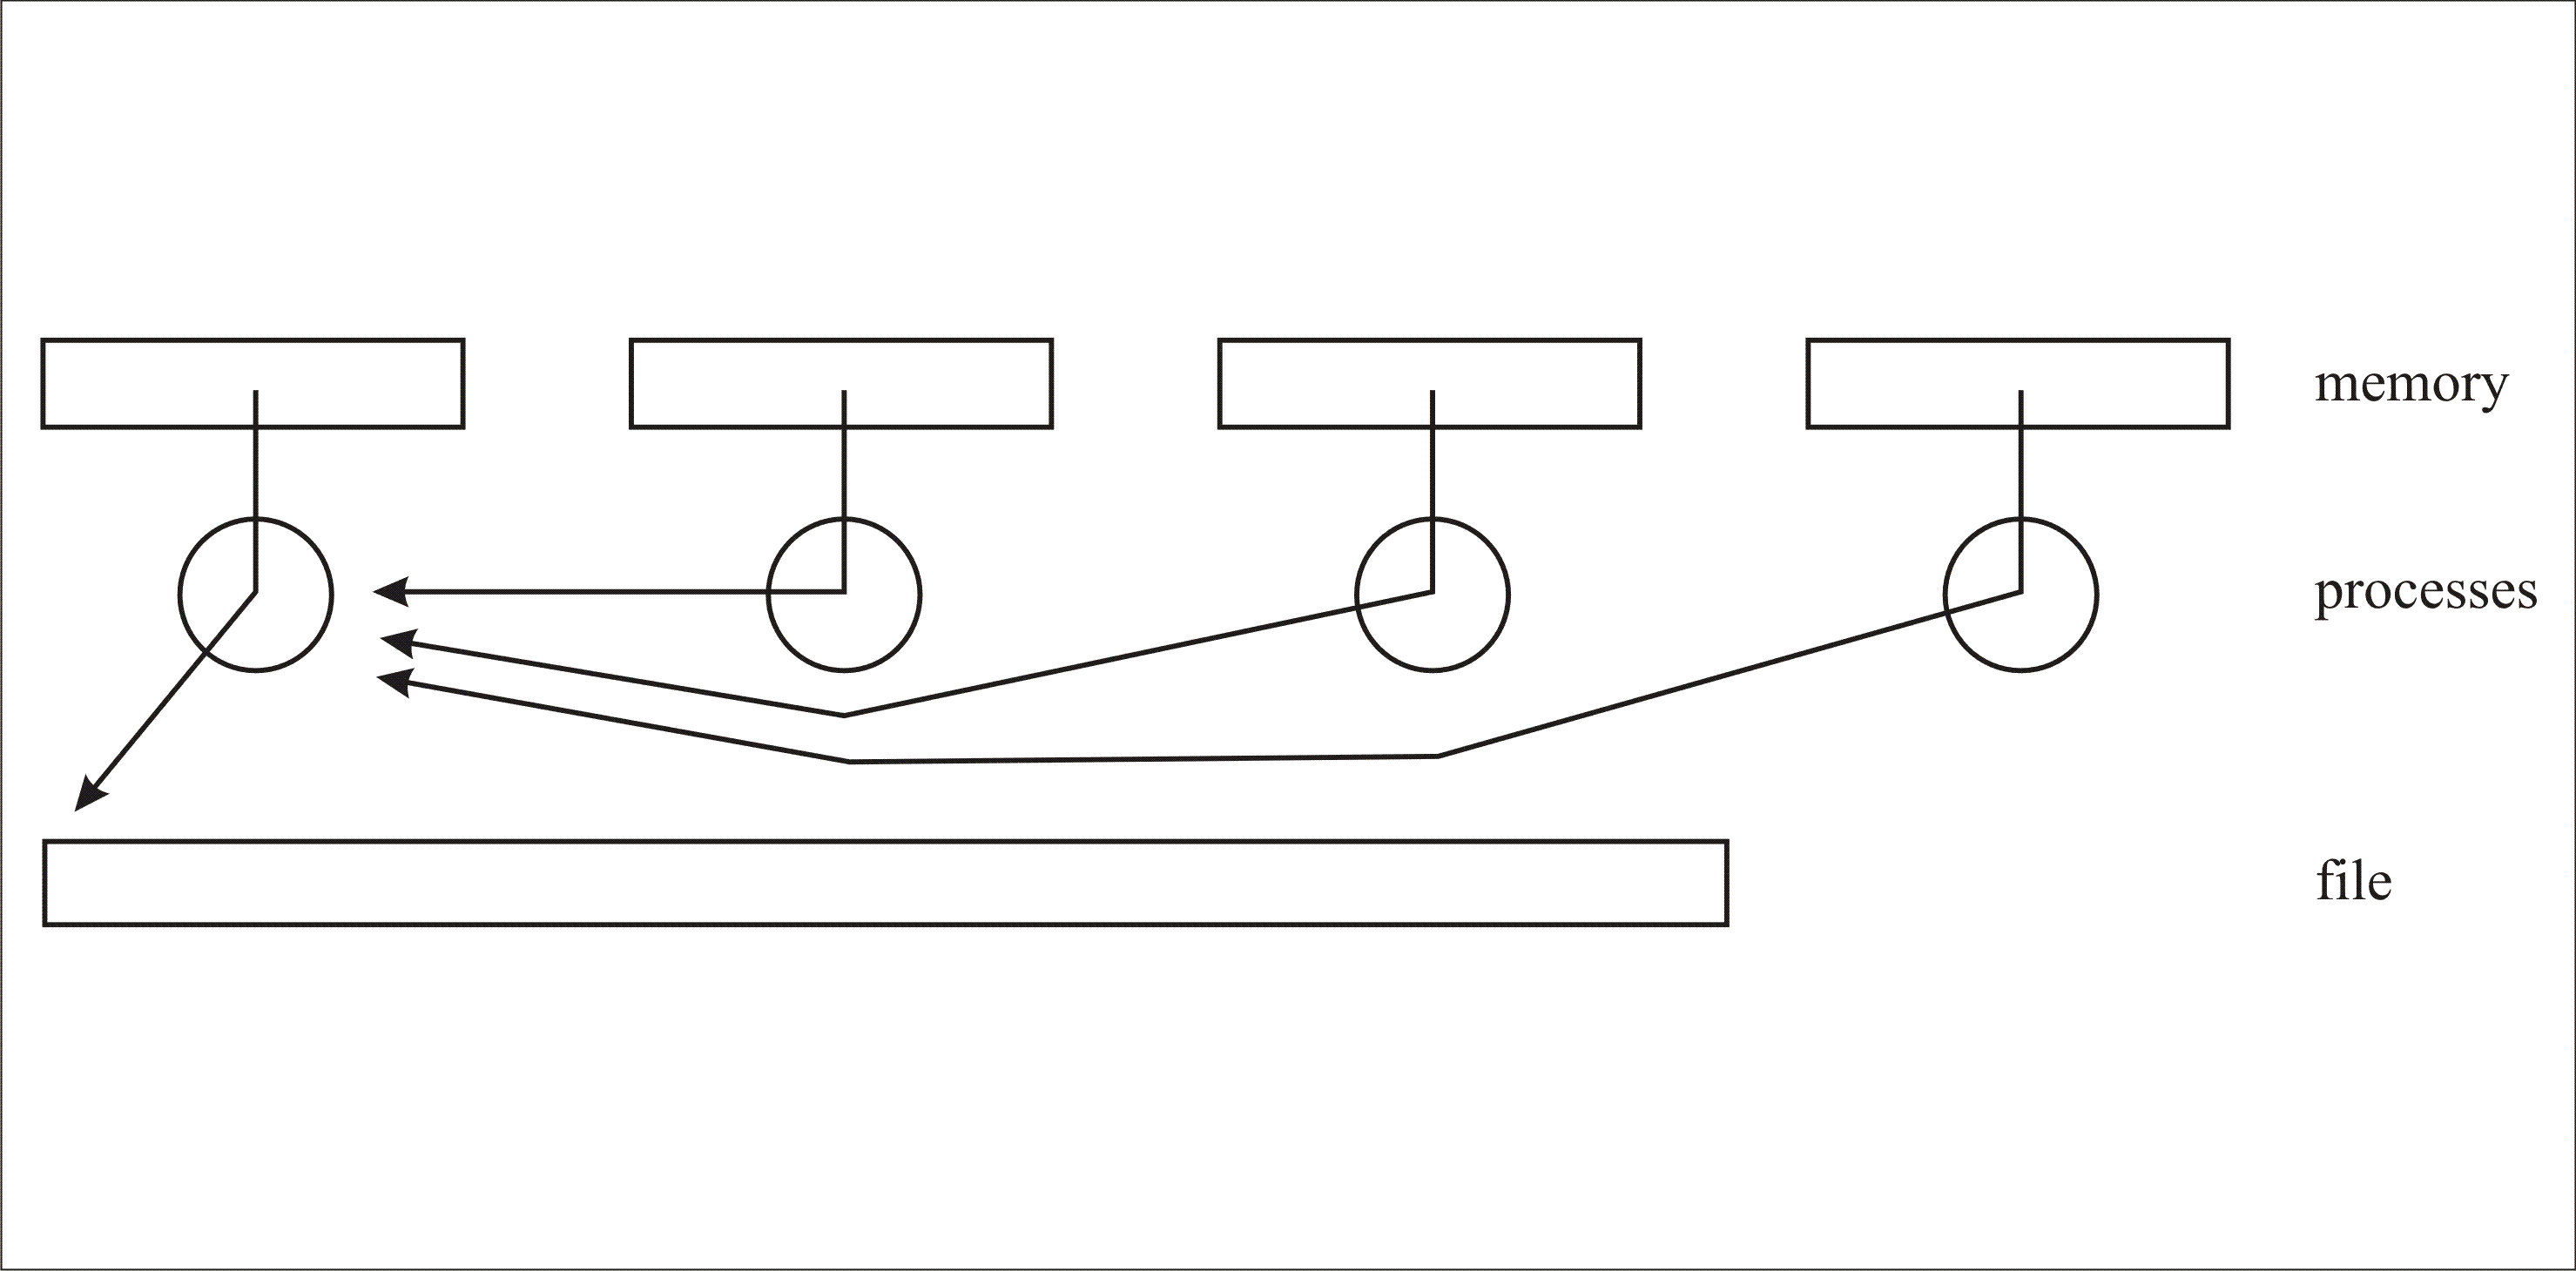
\includegraphics[width=1\textwidth]{slike/sequential_i_o.png}\\[1cm]
  \caption{Секвенцијалне улазно/излазне операције паралелног програма}
\end{figure}

\subsection{MPI програм - непаралелне У/И операције}

MPI-1 нема никакву експлицитну подршку за паралелне У/И операције, док су MPI апликације развијене у последњих неколико година морале да имају и свој У/И део програма. Ти делови програма су писани ослањајући се на карактеристике које пружа оперативни систем, најчешће UNIX. Најједноставније је имати један процес који извршава све У/И операције, док други процеси извршавају операције са учитаним подацима. Ако се узме пример писања низа бројева у фајл дужине 100, онда дужина података коју обрађује сваки процес зависи од укупног броја процеса. Програм почиње иницијализацијом дела низа за сваки процес. Сви процеси осим процеса 0 шаљу своје делове низа процесу 0. Процес 0 уписује свој део низа у фајл, а затим прихвата делове низа од других процеса. Ранг сваког процеса је одређен у  \texttt{MPI\_Recv} функцији, тако да се зна редослед пристизања делова низа. Ово је најчешћи начин да се непаралелне У/И операције врше у паралелном програму који је конвертован из секвенцијалног програма, јер промене нису  направљене на У/И делу програма. 

Уколико је $numprocs=1$, онда нема MPI комуникације. 

Неки од разлога зашто се У/И операције пишу на овај начин су:

\begin{itemize}
\item  Паралелни компјутери на којима је покренут програм можда подржавају У/И операције само са једног процеса.
\item Могу се користити софистициране У/И библиотеке које су можда писане као део високог нивоа слоја за управљање података, а које не подржавају паралелне У/И операције.
\item Резултујући фајл је погодан за руковање изван програма (нпр. \textit{mv}, \textit{cp}, или \textit{ftp}).
\end{itemize}

Учинак програма може бити побољшан омогућавањем процеса да складишти велики блок података. Уколико процес 0 има довољан бафер за податке, он може акумулирати податке других процеса у једниствен бафер за једну велику операцију писања(Листинг 3.1). Разлог због кога не треба писати У/И операције на овај начин је недостатак паралелизма који ограничава учинак и скалабилност, нарочито ако основни систем фајлова омогућава паралелне У/И операције.

\begin{lstlisting}[style=nonumbers,frame=single,language=C, caption= MPI програм ]
#include "mpi.h"
#include <stdio.h>
#define BUFSIZE 100
int main(int argc, char *argv[])
{
	int i, myrank, numprocs, buf[BUFSIZE];
	MPI_Status status;
	FILE *myfile;
	MPI_Init(&argc, &argv);
	MPI_Comm_rank(MPI_COMM_WORLD, &myrank);
	MPI_Comm_size(MPI_COMM_WORLD, &numprocs);

	for (i=0; i<BUFSIZE; i++)
	{
		buf[i] = myrank * BUFSIZE + i;
	}
	if (myrank != 0)
	{
		MPI_Send(buf, BUFSIZE, MPI_INT, 0, 99, MPI_COMM_WORLD);
	}
	else
	{
		myfile = fopen("testfile", "w");
		fwrite(buf, sizeof(int), BUFSIZE, myfile);
		for (i=1; i<numprocs; i++)
		{
			MPI_Recv(buf, BUFSIZE, MPI_INT, i, 99, MPI_COMM_WORLD,
			&status);
			fwrite(buf, sizeof(int), BUFSIZE, myfile);
		}
		fclose(myfile);
	}
	MPI_Finalize();
	return 0;
}
\end{lstlisting}

\subsection{MPI програм - без MPI улазно/излазних операција}
У циљу решавања овог недостатка, следећи корак у миграцији секвенцијалног програма ка паралелном је да се за сваки процес оперише са посебним фајлом, што омогућава паралелни пренос података(Листинг 3.2). Овде су У/И операције сваког процеса потпуно независне од У/И операција других процеса. Тако, је сваки програм секвенцијалан у односу на У/И операције. Наиме, процес отвара свој фајл, уписује податке у њега, а затим га и затвара. Најбоље је да се у називу излазног фајла налази и ранг процеса. Предност овог приступа је да се У/И операције могу одвијати паралелно, а и даље се могу користити секвенцијалне У/И библиотеке. Основни недостатак оваквог приступа је креирање више фајлова уместо једног. Поред тога, недостаци овакве шеме су:

\begin{itemize}
\item Фајлови се морају спојити пре него што буду коришћени као улаз у другом програму.
\item Може се десити да програм који чита ове фајлове мора бити паралелни и стартован са истим бројем процеса.
\item Тешко је држати скуп фајлова као групу, ради копирања, премештања и слања путем мреже.

\end{itemize}

\begin{lstlisting}[style=nonumbers,frame=single,language=C,caption= MPI програм без MPI улазно/излазних операција]
#include "mpi.h"
#include <stdio.h>
#define BUFSIZE 100
int main(int argc, char *argv[])
{
	int i, myrank, buf[BUFSIZE];
	char filename[128];
	FILE *myfile;
	MPI_Init(&argc, &argv);
	MPI_Comm_rank(MPI_COMM_WORLD, &myrank);
	for (i=0; i<BUFSIZE; i++)
	{
		buf[i] = myrank * BUFSIZE + i;
	}
	sprintf(filename, "testfile.%d", myrank);
	myfile = fopen(filename, "w");
	fwrite(buf, sizeof(int), BUFSIZE, myfile);
	fclose(myfile);
	MPI_Finalize();
	return 0;
}
\end{lstlisting}


Учинак може бити мањи уколико имамо велики број процеса. То ће довести до великог броја У/И операција са малим бројем података. 

\subsection{MPI У/И операције са одвојеним фајловима}
MPI У/И програм је сличан као и претходни програм, с тим што се све У/И операције извршавају MPI функцијама(Листинг 3.3). Овакав програм има неколико предности и мана.
 
Прва разлика је у овим фајловима је та што је декларација \texttt{FILE} замењена са \texttt{MPI\_File} као типом \textit{myfile}. Сада је \textit{myfile} променљива типа MPI\_File, уместо показивач на објекат типа FILE.

\begin{lstlisting}[style=nonumbers,frame=single,language=C, caption= MPI програм са одвојеним фајловима]
#include "mpi.h"
#include <stdio.h>
#define BUFSIZE 100
int main(int argc, char *argv[])
{
	int i, myrank, buf[BUFSIZE];
	char filename[128];
	MPI_File myfile;
	MPI_Init(&argc, &argv);
	MPI_Comm_rank(MPI_COMM_WORLD, &myrank);
	for (i=0; i<BUFSIZE; i++)
	{
		buf[i] = myrank * BUFSIZE + i;
	}
	sprintf(filename, "testfile.%d", myrank);
	MPI_File_open(MPI_COMM_SELF, filename,
	MPI_MODE_WRONLY | MPI_MODE_CREATE,MPI_INFO_NULL, &myfile);
	MPI_File_write(myfile, buf, BUFSIZE, MPI_INT,
	MPI_STATUS_IGNORE);
	MPI_File_close(&myfile);
	MPI_Finalize();
	return 0;
}
\end{lstlisting}


MPI функција која замењује функцију fopen назива се \texttt{MPI\_File\_open}.

\begin{verbatim}
MPI_File_open(MPI_COMM\_SELF, filename,MPI_MODE_CREATE | MPI_MODE_WRONLY,
MPI_INFO_NULL, &myfile);
\end{verbatim}

Аргументи ове функције су:

\begin{itemize}
\item \textbf{Комуникатор} - Ovo je најзначајнија компонента У/И операција у MPI. Фајлови су отворени скупом процесора идентификованих од стране комуникатора. 
Ово обезбеђује да процеси раде на фајлу заједно омогућујући и комуникацију између процеса. 
Пошто сваки процес отвара свој фајл, онда се користи комуникатор \texttt{MPI\_COMM\_SELF}.

\item \textbf{Назив фајла} - Други аргумент је стринг који представља назив фајла као и у функцији \textit{fopen}.

\item \textbf{Тип мода} - Трећи аргумент је мод у коме је фајл отворен. У овом програму значи да је креиран или преписан ако већ постоји, као и да ће писање у фајл бити извршено само од стране овог програма. Константе  \texttt{MPI\_MODE\_CREATE} и \texttt{MPI\_MODE\_WRONLY} представљају заставице.

\item  \textbf{MPI\_INFO\_NULL} - MPI\_INFO\_NULL је предефинисана константа која представља лажну вредност за инфо аргумент \texttt{MPI\_File\_open}. 

\item \textbf{Фајл променљива} - Као последњи аргумент је адреса \texttt{MPI\_File} променљиве, коју ће функција  \texttt{MPI\_File\_open} отворити. Као и све MPI функције у C програму, \texttt{MPI\_File\_open} има повратну вредост. Уколико је фајл успешно отворен повратна вредност је \texttt{MPI\_SUCCESS}.

\end{itemize}
 
Следећа функција која је важна за функционисање за MPI У/И је:

 \begin{verbatim}
MPI_File_write(myfile, buf, BUFSIZE, MPI_INT,MPI_STATUS_IGNORE);
\end{verbatim}

Податак који се уписује мора бити одређен адресом, величином и типом. Овим начином се описује бафер који ће бити коришћен за писање(Листинг 3.4). То омогућава да се несуседни подаци у меморији запишу само једним позивом. Конкретно, овде се уписују 
\texttt{BUFSIZE} целих бројева са почетком у адреси \textit{buf}. Последњи аргумент функције је статус, који је истог типа као и код \texttt{MPI\_Recv}.
У овом сличају занемариће се повратна вредност. MPI-2 је одредио специјалну вредност статуса \texttt{MPI\_STATUS\_IGNORE}. Ова вредност може бити послата ако аргумент било којој MPI функцији у циљу игнорисања повратне вредности одговарајуће функције.
Технички, ово упрошћење може побољшати учинак програма уколико нам статус није потребан.

Функција \texttt{MPI\_File\_close(\&myfile)} служи за затварање фајла. Послата адреса \textit{myfile} биће преписана са  \texttt{MPI\_FILE\_NULL} уколико се затварање фајла не обави успешно. Тако се могу идентификовати неважећи фајлови.

\begin{lstlisting}[style=nonumbers,frame=single,language=C, caption=MPI програм за паралелним MPI функцијама]
#include "mpi.h"
#include <stdio.h>
#define BUFSIZE 100
int main(int argc, char *argv[])
{
	int i, myrank, buf[BUFSIZE];
	MPI_File thefile;
	MPI_Init(&argc, &argv);
	MPI_Comm_rank(MPI_COMM_WORLD, &myrank);
	for (i=0; i<BUFSIZE; i++)
	{
		buf[i] = myrank * BUFSIZE + i;
	}
	MPI_File_open(MPI_COMM_WORLD, "testfile",
	MPI_MODE_CREATE | MPI_MODE_WRONLY,
	MPI_INFO_NULL, &thefile);
	MPI_File_set_view(thefile, myrank * BUFSIZE * sizeof(int),
	MPI_INT, MPI_INT, "native", MPI_INFO_NULL);
	MPI_File_write(thefile, buf, BUFSIZE, MPI_INT,
	MPI_STATUS_IGNORE);
	MPI_File_close(&thefile);
	MPI_Finalize();
	return 0;
}
\end{lstlisting}


\subsection{Паралелне MPI У/И операције са једним фајлом}

Да би се добио још бољи учинак MPI У/И операција, потребно је изменити програм тако да процеси деле један фајл, уместо да пишу у више њих(слика 3.2). Тако се отклањају све мане код уписа у више фајлова и постиже се потпуни паралелизам.

Прва разлика између програма који уписује у више различитих фајлова је први аргумент функције \texttt{MPI\_File\_open}. Пошто сада сваки процес не приступа свом фајлу, већ једном дељеном за све процесе, уместо комуникатора \texttt{MPI\_COMM\_SELF} користи се комуникатор  \texttt{MPI\_COMM\_WORLD}. Тиме се постиже да сви процеси отварају исти фајл.

\begin{figure}[h!]
  \centering
      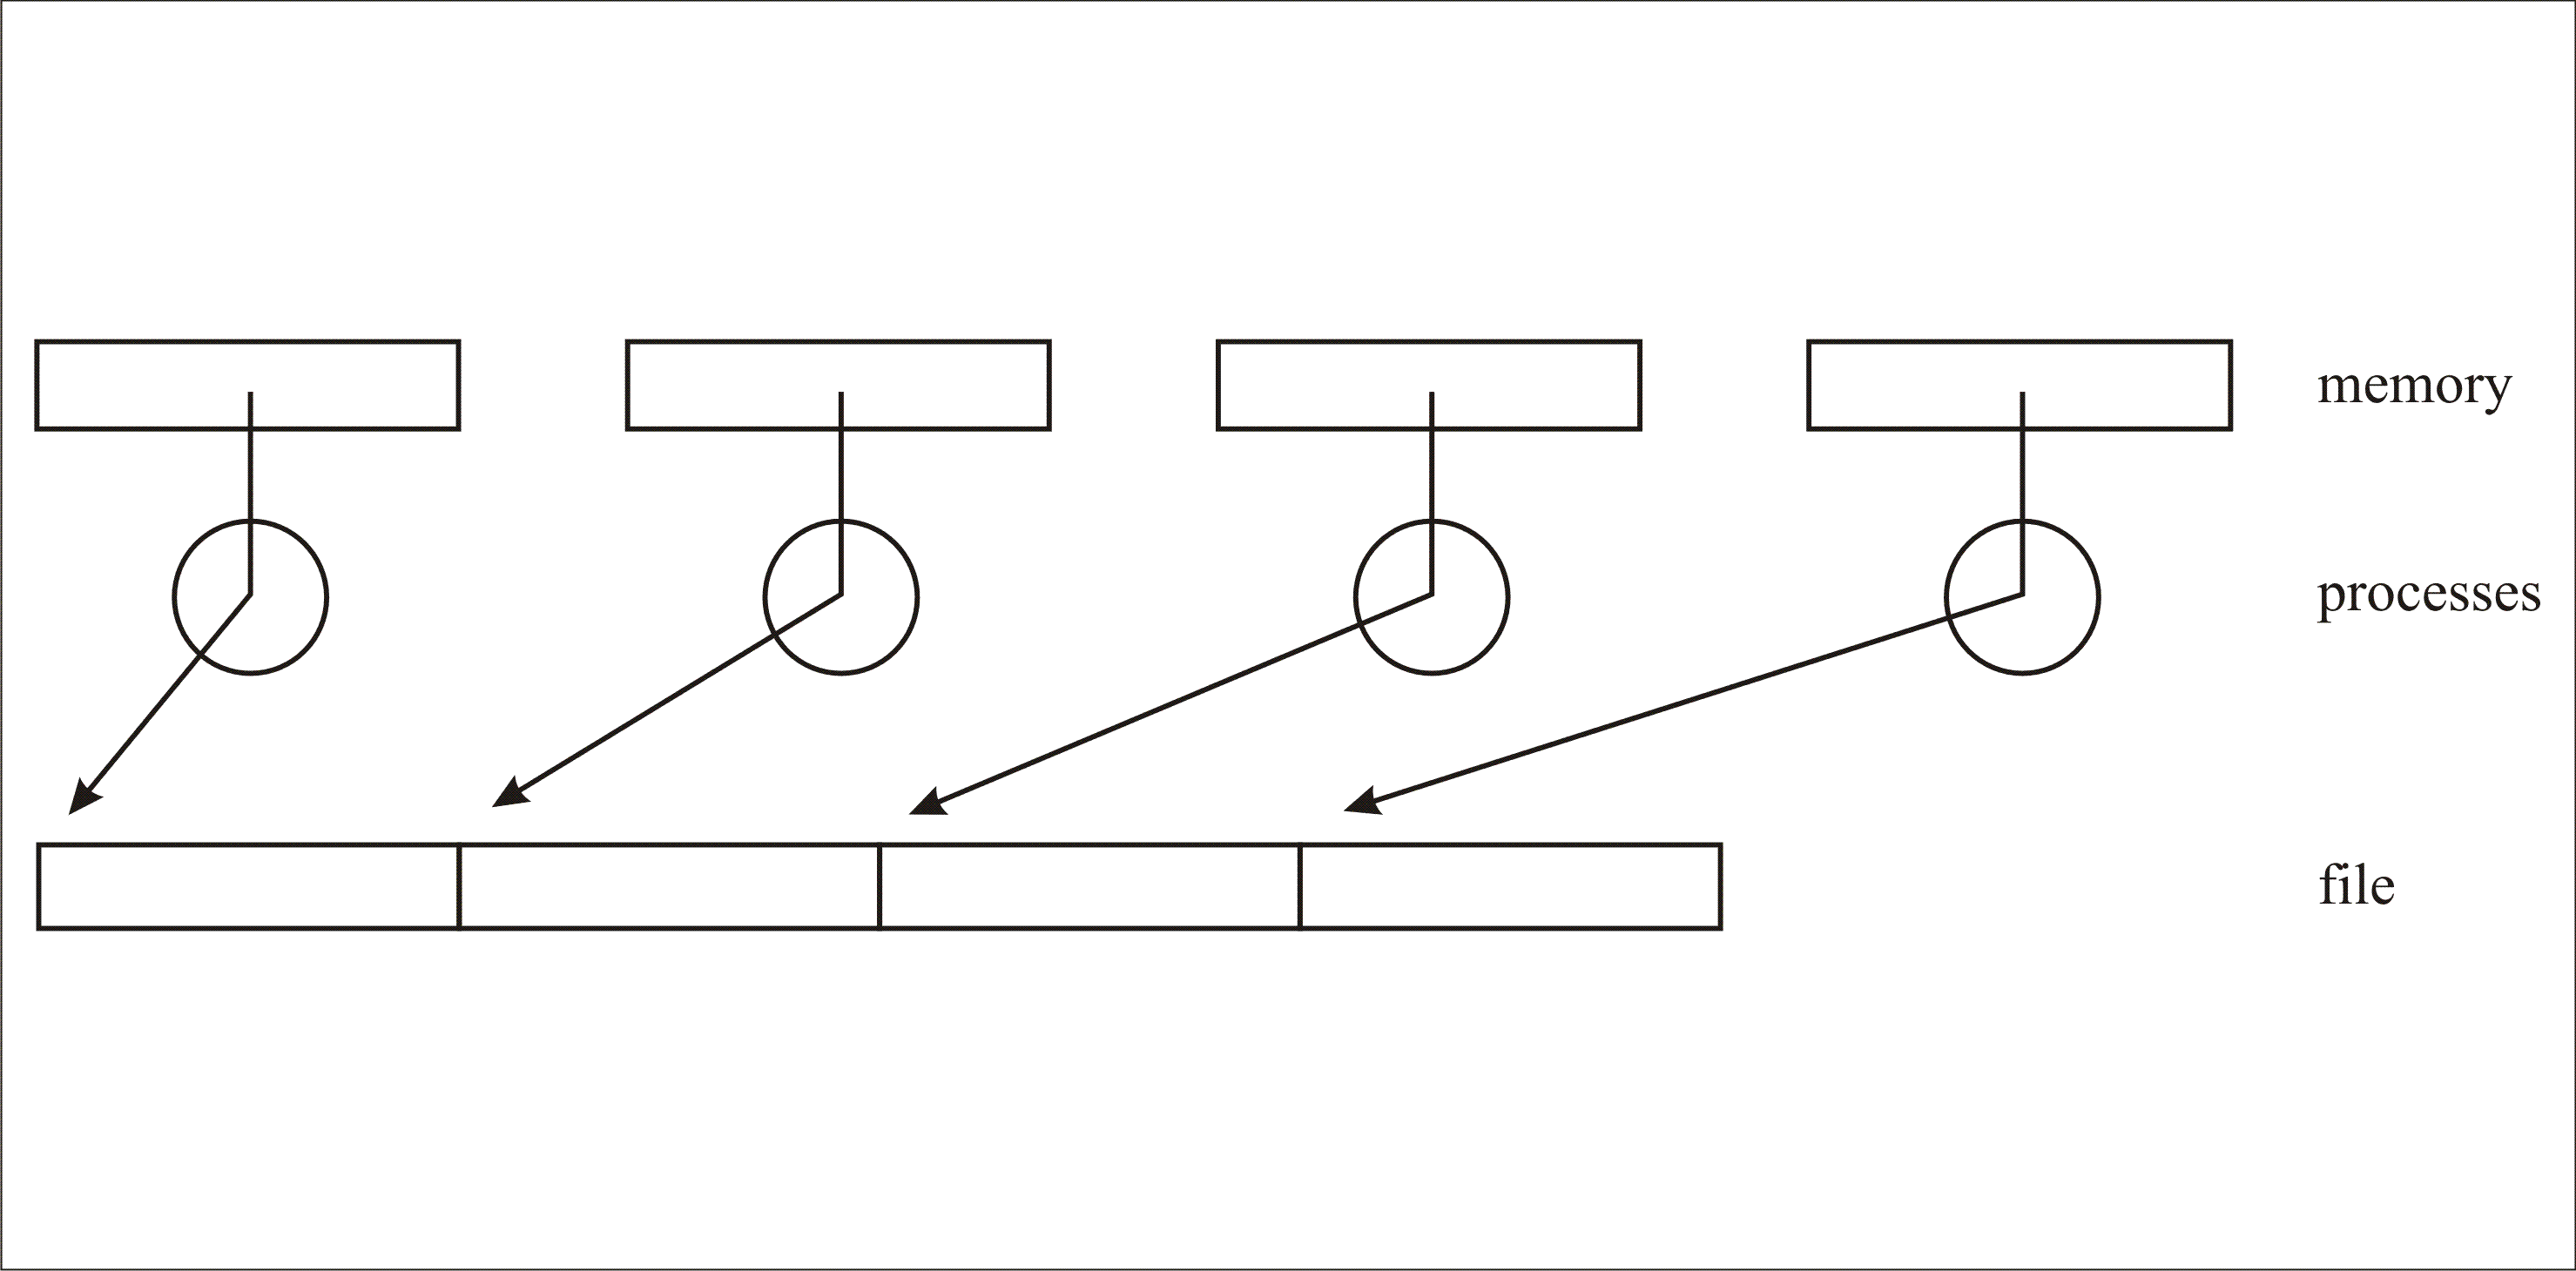
\includegraphics[width=1\textwidth]{slike/paralel_i_o_single_file.png}\\[1cm]
  \caption{Паралелне MPI У/И операције са једним фајлом}
\end{figure}

Ово је колективна операција  на комуникатору, тако да сви процеси који учествују позивају \texttt{MPI\_File\_open}, при чему се, као што је напоменуто, отвара се само један фајл. Део фајла може се видети у процесу, што се назива \textbf{поглед фајла}. Поглед фајла се поставља функцијом \texttt{MPI\_File\_set\_view}.

\begin{verbatim}
MPI_File_set_view(thefile, myrank * BUFSIZE * sizeof(int), MPI_INT,
 MPI_INT, "native", MPI_INFO_NULL);
\end{verbatim}

Први аргумент идентификује фајл. Други аргумент је место (у бајтовима) у фајлу од кога почиње део фајла асоциран датом процесу.
Овде множимо величину података (BUFSIZE * sizeof (int)) по рангу процеса, тако да поглед на сваки процес почиње на одговарајућем месту у фајлу.
Тај аргумент је типа \texttt{MPI\_Offset}, који на системима који подржавају велике фајлове очекује 64-битни цели број. Следећи аргумент се назива \textbf{etype погледа}. То је скуп свих типова података који се налазе у фајлу. У овом случају то је \texttt{MPI\_INT}, што значи да ће се у фајл увек уписати цели број. Следећи аргумент се назива \textit{filetype}, и то је веома флексибилан начин да се опишу дисконтинуални погледи у фајлу. У овом случају ради се само о типу \texttt{MPI\_INT}, тако да нема дисконтинуалних података за упис. Генерално, \textit{etype} и \textit{filetype} могу да буду било који предефинисани MPI типови података. Аргумент који означава представљање података у фајлу и најчешће је типа стринг назива се \zn природни". Нативно представљање значи да се подаци уписују у фајл тачно онако како су представљени у меморији. Ова шема чува податке и сумарни учинак програма, јер се не губи време ни на какве додатне конверзије.
Остала представљања су \textit{унутрашња} и \textit{external32}, која омогућавају различите врсте преноса између машина са различитим архитектурама и типовима представљања.
Последњи аргумент је инфо аргумент као и у функцији \texttt{MPI\_File\_open}.

Неке MPI функције у програмском језику C се налазе у Листингу 3.5:

\begin{lstlisting}[style=nonumbers,frame=single, language=C, caption=MPI функције]
int MPI_File_open(MPI_Comm comm, char *filename, int amode, MPI_Info info,
MPI_File *fh)

int MPI_File_set_view(MPI_File fh, MPI_Offset disp, MPI_Datatype etype,
MPI_Datatype filetype, char *datarep, MPI_Info info)

int MPI_File_write(MPI_File fh, void *buf, int count, MPI_Datatype datatype,
MPI_Status *status)
int MPI_File_close(MPI_File *fh)

int MPI_File_get_size(MPI_File fh, MPI_Offset *size)
int MPI_File_read(MPI_File fh, void *buf, int count, MPI_Datatype datatype,
MPI_Status *status)
\end{lstlisting}

Овим начином, написани програм је независан од броја процеса на којима је покренут. Укупна величина датотеке се добија тако да сваки процес ради са скоро истом величином података.
MPI функција која се користи за добијање величине фајла је  \texttt{MPI\_File\_get\_size}. Први аргумент ове функције је отворени фајл, а другi je адреса где треба сместити израчунату величину фајла у бајтовима. Пошто многи системи сада могу управљати датотекама чије су дужине превелике да би биле
представљене као 32-битни цео број, MPI дефинише тип,  \texttt{MPI\_Offset}, који може да а садржи величину фајла у 64 бита. 
То је тип који се користи 
за аргументе MPI функција који се односе на померање у фајловима. У супротном, програм који се користи за читање фајла је веома сличан оном који пише. Разлика између писања и читања је да процес не зна увек тачно колико ће података буде прочитано.

\subsection{Коришћење појединачних фајл показивача}

MPI програм са улазно/излазним операцијама је могуће писати и са појединачним фајл показивачима(Листинг 3.6). Сваки од ових програма има део за У/И операције које отварају, читају и на крају затварају фајл. \texttt{MPI\_File\_open} је функција која отвара фајл. Први аргумент је комуникатор који идентификује групу процеса којима је потребан приступ фајлу. \texttt{MPI\_COMM\_WORLD} се користи зато што је свим процесима потребан приступ фајлу \textit{/pfs/datafile}. MPI стандард не одређује формат за назив фајла. Свака од MPI имплементација има слободу да дефинише формат који они подржавају. Може се очекивати да ће имплементација подржати познате конвенције именовања. Имплементације које се покрећу на Unix окружењу подржавају Unix конвенцију именовања. \textit{/pfs/datafile} је фајл који се налази у директоријуму \textit{pfs}. У имплементацијама је назив директоријума опциони део назива фајла. Уколико не постоји, имплементација ће користити директоријум у коме се процес тренутно налази. Трећи аргумент функције \texttt{MPI\_File\_open} је начин приступа. У овом сличају то је \texttt{MPI\_MODE\_RDONLY}, зато што је довољно да програм само чита из фајла. Четврти аргумент је инфо аргумент. Последњи аргумент је показивач на фајл који враћа функција \texttt{MPI\_File\_open}.


\begin{lstlisting}[style=nonumbers,frame=single,language=C, caption= MPI програм са појединачним фајл показивачима]
#include "mpi.h"
#define FILESIZE (1024 * 1024)
int main (int argc, char **argv)
{
int *buf, rank, nprocs, nints, bufsize;
MPI_File fh;
MPI_Status status;
MPI_Init(&argc,&argv);
MPI_Comm_rank(MPI_COMM_WORLD, &rank);
MPI_Comm_size(MPI_COMM_WORLD, &nprocs);
bufsize = FILESIZE/nprocs;
buf = (int *) malloc (bufsize);
nints = bufsize/sizeof (int);
MPI_File_open(MPI_COMM_WORLD, "/pfs/datafile", MPI_MODE_RDONLY,
MPI_INFO_NULL, &fh);
MPI_File_seek(fh, rank*bufsize, MPI_SEEK_SET);
MPI_File_read(fh, buf, nints, MPI_INT, &status);
MPI_File_close(&fh);
free (buf);
MPI_Finalize();
return 0;
}
\end{lstlisting}

Овај C програм извршава улазно/излазне операције користећи појединачне показиваче на фајл. После отварања фајла, сваки процес копира глобални фајл показивач у локални фајл показивач који показује на локацију у фајлу од које сваки процес чита свој део фајла. Први аргумент функције \texttt{MPI\_File\_seek} је показивач на фајл који је отворила функција 
\texttt{MPI\_File\_open}. Други аргумент одређује део фајла који сваки процес чита. \texttt{MPI\_SEEK\_SET} значи да се почетак локације за читање рачуна од почетка фајла. У C програмском језику 
за ово се користи предефинисан тип \texttt{MPI\_Offset}. Имплементација дефинише \texttt{MPI\_Offset} као цео број који је довољно велики да подржи највећу дужину фајла. Део фајла сваког процеса се одређује производом ранга процеса и величине податка у бајтовима. Величина податка може се одредити и функцијама \texttt{MPI\_Get\_countor} \texttt{MPI\_Get\_elements}, користећи статус објекат који враћа функција \texttt{MPI\_File\_read}.


\subsection{Употреба експлицитних одступања}

\texttt{MPI\_File\_read} и \texttt{MPI\_File\_write} се називају појединачним фајл показивачима због тога што користе показивач на локацију у фајлу од које сваки процес чита фајл(Листинг 3.7). MPI такође специфицира  неколико функција које се називају \textbf{експлицитним функцијама одступања} (\texttt{MPI\_File\_read\_at} и \texttt{MPI\_File\_write\_at}). Ове функције не користе појединачне фајл показиваче. У њима, локација у фајлу се директно прослеђује функцији као аргумент. Уколико више нити процеса приступају истом фајлу, онда се морају користити појединачни фајл показивачи због безбедности нити.

\begin{lstlisting}[style=nonumbers,frame=single,language=C, caption= MPI функције]
int MPI_File_read_at(MPI_File fh, MPI_Offset offset, void *buf, int count,
MPI_Datatype datatype, MPI_Status *status)
int MPI_File_write_at(MPI_File fh, MPI_Offset offset, void *buf, int count,
MPI_Datatype datatype, MPI_Status *status)
\end{lstlisting}

\subsection{Писање у фајл}
Уколико је потребно уписати податке у фајл, онда се користе функције \texttt{MPI\_File\_write} и \texttt{MPI\_File\_write\_at}. Уместо заставице \texttt{MPI\_MODE\_RDONLY} која је служила за читање фајла, за упис података у фајл се користе заставице \texttt{MPI\_MODE\_CREATE} и \texttt{MPI\_MODE\_WRONLY}. \texttt{MPI\_MODE\_CREATE} се користи за креирање фајла уколико он већ не постоји. \texttt{MPI\_MODE\_WRONLY} означава да је фајл отворен за писање. У C програмском језику, обе заставице могу се користити битовним или оператором :  \texttt{MPI\_MODE\_CREATE} | \texttt{MPI\_MODE\_WRONLY}. Да би функција \texttt{MPI\_File\_open} креирала фајл, потребно је да постоји директоријум који је наведен у називу фајла.

\subsection{Неконтинуални приступи и колективне У/И операције}

У великом броју реалних паралелних апликација, сваком процесу је потребно да приступи малим деловима података који су смештени у фајлу неконтинуално  [4, 17, 65, 77, 78, 85].
Један начин да се приступи неконтунуалним подацима је користећи функције за читање/писање малих континуалних делова, као у Unix системима. Због велике латенције улазно/излазних операција, приступање малим деловима података захтева много времена. Предност MPI на Unix системима је могућност приступа неконтинуалним деловима података позивајући само једну функцију. 

\subsubsection{Неконтинуални приступи}
MPI програм поседује концепт погледа на фајл. Поглед фајла у MPI-у је дефинисан као део фајла коме процес има приступ(слика 3.3). Користећи поглед на фајл, функције читања и писања могу приступити само том делу фајла. Сви остали подаци се прескачу. Када се отвори, фајл је доступан процесу и MPI третира фајл као скуп бајтова (не као цели бројеви, реални бројеви итд.). Приликом покретања програма, сваки пројединачни фајл показивач је постављен на 0. Ово се може променити помоћу функције \texttt{MPI\_File\_set\_view}(Листинг 3.8). Најчешће се то ради из два разлога:

\begin{itemize}
\item Да се одреди тип податка коме је потребно приступити, нпр. целим или децималним бројевима. 
Ово је нарочито неопходно за преносивост фајла уколико корисник жели да приступи фајлу са друге машине и са различитим представљањем фајла. 

\item Да се одреде делови фајла који ће бити прескочени, тј. одређивање неконтунуалног приступа фајлу. За појединачне фајл показиваче или експлицитна одступања, сваки процес може користети различит тип погледа.
\end{itemize}

За приступ подацима са подељеним фајл показивачем потребно је да сви процеси користе исти поглед. Поглед фајла се може мењати небројано пута.
MPI типови података се користе за одређивање погледа фајла. Поглед је одређен са:

\begin{itemize}
\item премештање
\item \textit{etype}
\item \textit{filetype}
\end{itemize}

\textbf{Премештање} одређује број бајтова који ће бити прескочени на почетку фајла. Ово се користи када је потребно да се прескочи читање заглавља фајла.
\textbf{Еtype} је основна јединица за приступ подацима. Може бити основни или изведени MPI тип података. Сви приступи фајлу се врше преко јединица типа etype. Сва одступања фајла се дефинишу као број \textit{ etype-ова}. Уколико је \textit{etype} MPI\_INT, појединачни и подељен фајл показивач биће померен за одређени број целих бројева.
\textbf{Filetype} je основни или изведени тип података који дефинише који део фајла је доступан процесу и ког типа су подаци. \textit{Filetype} мора бити исти као etype или изведен од типа који се заснива на \textit{etype}.
Поглед фајл почиње од премештања и састоји се од више суседних \textit{etype}. Приликом отварања фајла, премештање има вредност 0  и \textit{etype} и \textit{filetype} су типа \texttt{MPI\_BYTE}. Ово је познато као подразумевани поглед фајла. 

\begin{figure}[h!]
  \centering
      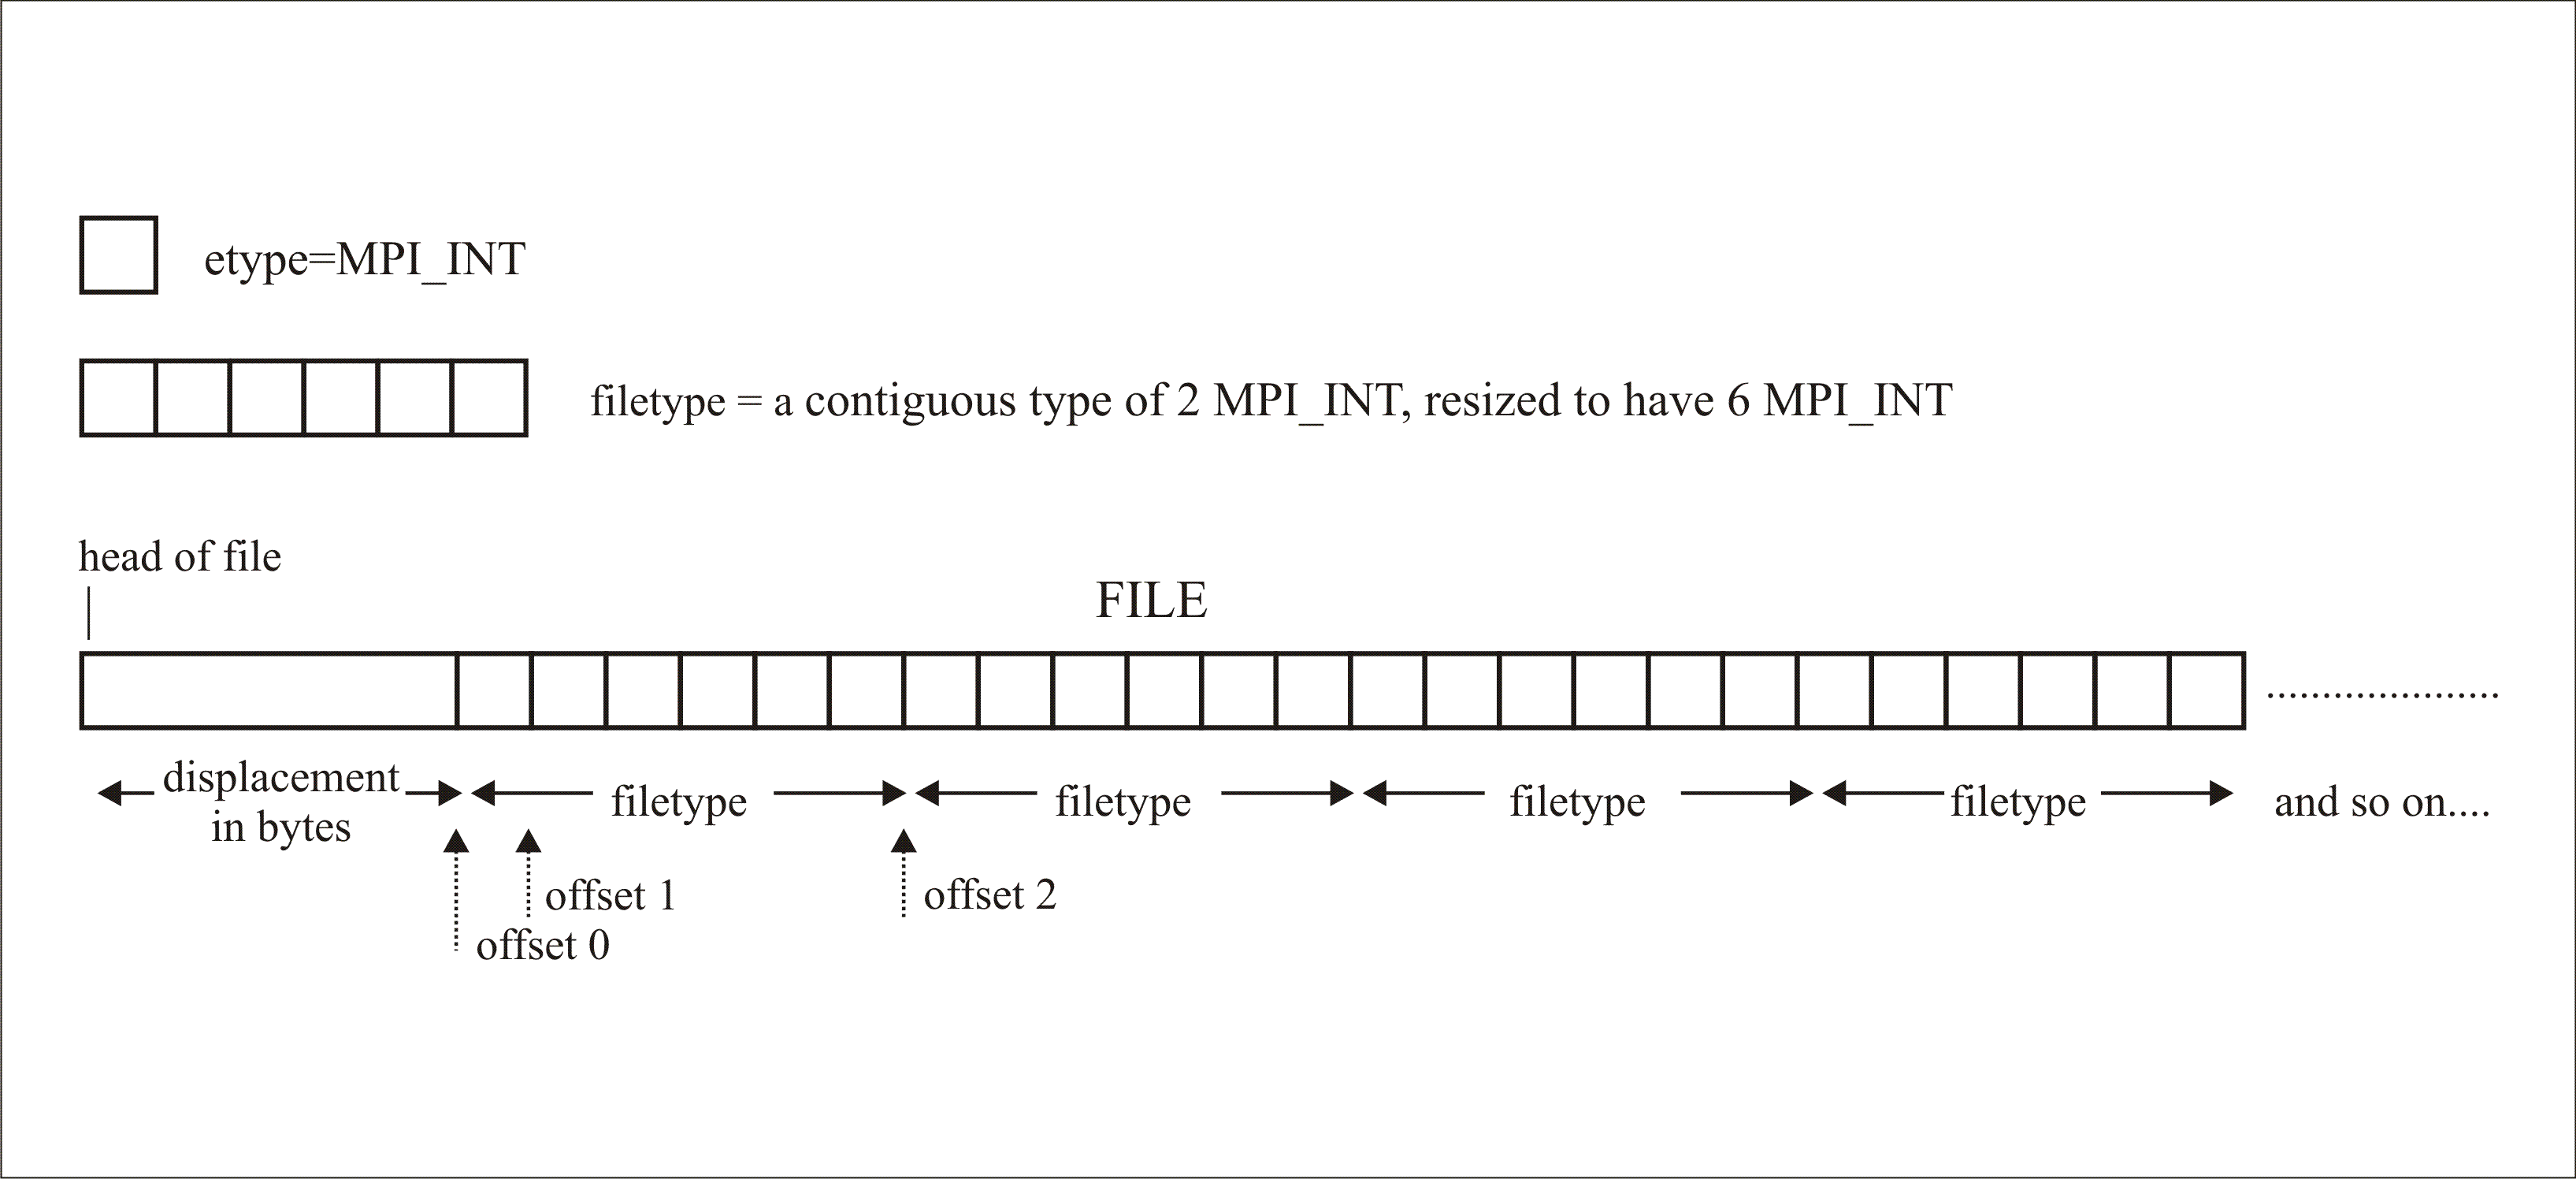
\includegraphics[width=1\textwidth]{slike/displacement.png}\\[1cm]
  \caption{Поглед фајла}
\end{figure}

На слици 3.3 је приказан суседни изведени тип података који је представљен као два цела броја. Уколико се поставе још 4 цела броја на крај овог типа података, функцијом\texttt{ MPI\_Type\_create\_resized} се добија тип податка који је величине шест целих бројева. \texttt{Еtype} је типа \texttt{MPI\_INT}, а премештање је 5*sizeof (int). У MPI-1 верзији ово се ради са функцијом \texttt{MPI\_Type\_struct}.

\begin{lstlisting}[style=nonumbers,frame=single, language=C, caption= MPI функције]
int MPI_File_set_view(MPI_File fh, MPI_Offset disp, MPI_Datatype etype,
MPI_Datatype filetype, char *datarep, MPI_Info info)
int MPI_Type_create_resized(MPI_Datatype oldtype, MPI_Aint lb,
MPI_Aint extent, MPI_Datatype *newtype)
\end{lstlisting}

Аргументи који се прослеђују функцији \texttt{MPI\_File\_set\_view} су:
\begin{itemize}
	\item показивач на фајл
	\item премештање
	\item \textit{etype}
	\item \textit{filetype}
	\item предствљање података
	\item инфо аргумент
\end{itemize}
Подразумевано представљање је нативно, док је подразумевани инфо аргумент \texttt{MPI\_INFO\_NULL}.

\subsubsection{Kолективне У/И операције}

Разлика између колективних У/И операција са неконтинуалним приступом и других У/И операција је у томе што код колективних операција сваки процес чита мале блокове података, који се налазе у фајлу по принципу \textit{round-robin} распоређивања(слика 3.4). Са Unix У/И операцијама, једини начин да се читају подаци је читање сваког блока одвојено, због тога што Unix функције омогућавају приступ само једном континуалном делу података. 

\begin{figure}[h!]
  \centering
      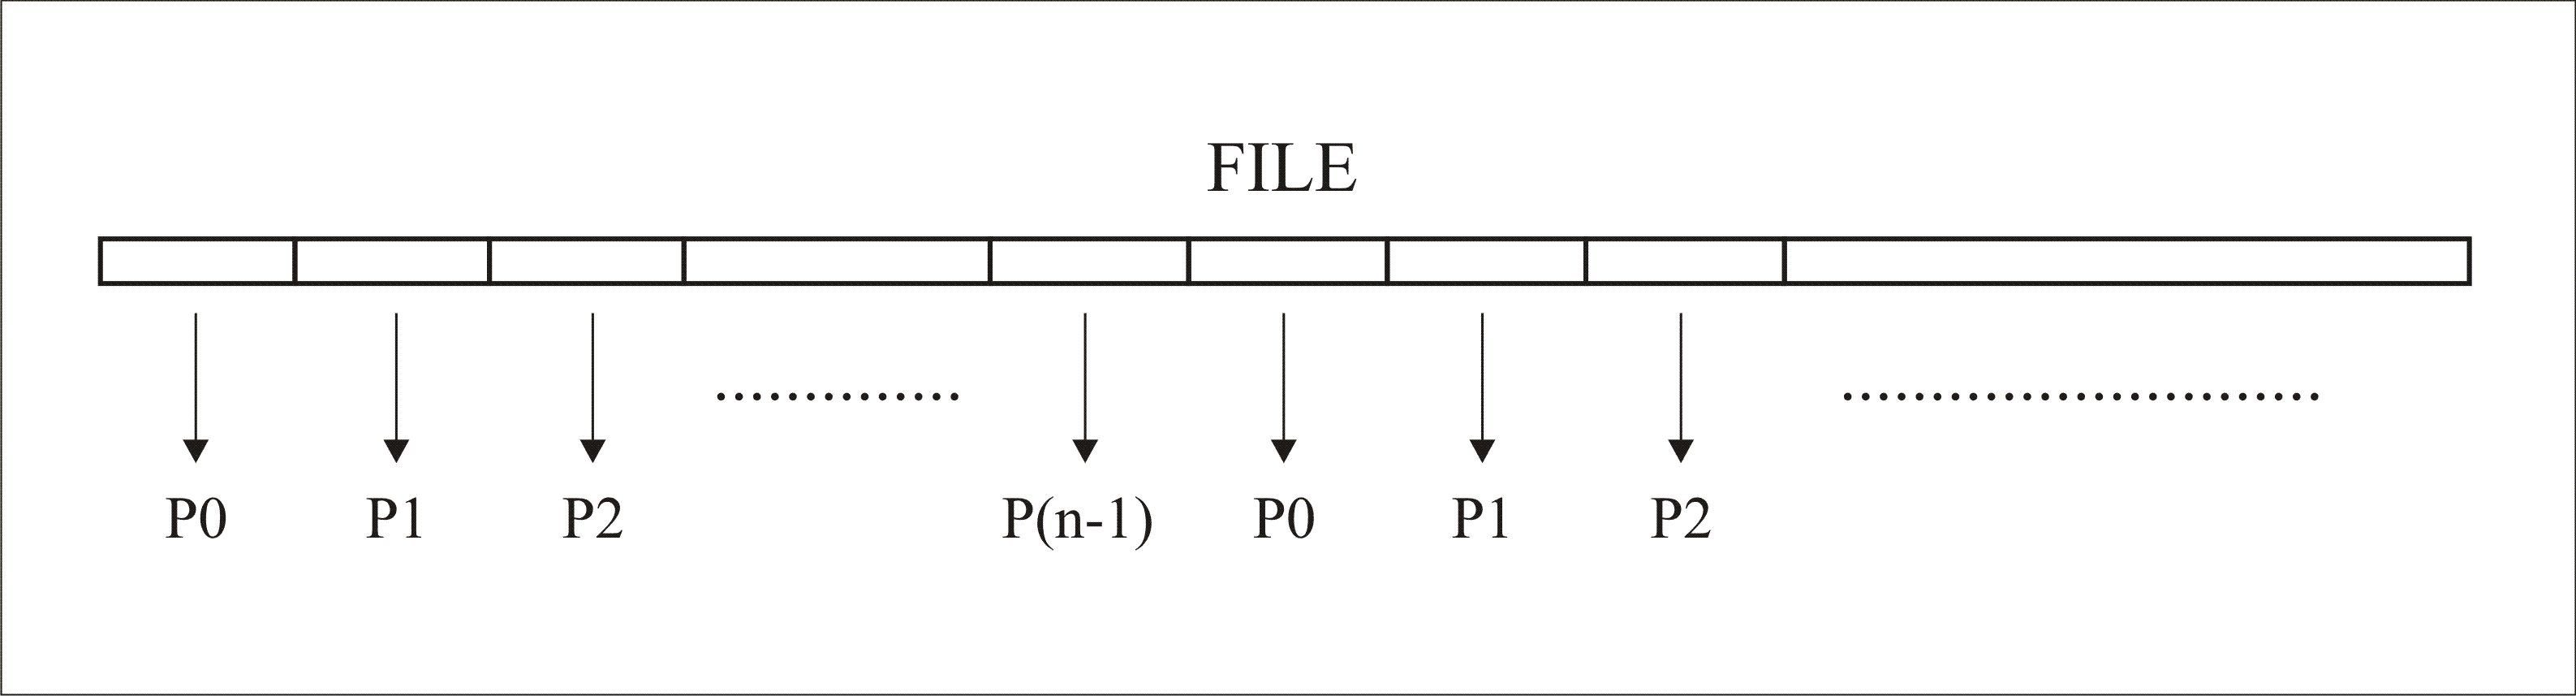
\includegraphics[width=1\textwidth]{slike/block-cyclic.png}\\[1cm]
  \caption{Колективне У/И операције}
\end{figure}

Код MPI-a, уместо позивања функције за читање више пута, може се дефинисати поглед на неконтунуални фајл сваког процеса, како би се прочитао фајл позивајући функцију само једном(Листинг 3.9). Други начин је употреба колективног читања. MPI имплементација даје много бољи учинак у односу на Unix У/И функције.

\texttt{FILESIZE} одређује величину фајла у бајтовима. \texttt{INTS\_PER\_BLK }је величина сваког блока који процес треба да прочита (број целих бројева у блоку). Сваки процес треба да прочита неколико блокова у цикличном распореду.

\begin{lstlisting}[style=nonumbers,frame=single,language=C, caption=MPI програм са погледом фајла]
#include "mpi.h"
#define FILESIZE
#define INTS_PER_BLK 104857616

int main(int argc, char **argv)
{
	int *buf, rank, nprocs, nints, bufsize;
	MPI_File fh;
	MPI_Datatype filetype;
	MPI_Init(&argc,&argv);
	MPI_Comm_rank(MPI_COMM_WORLD, &rank);
	MPI_Comm_size(MPI_COMM_WORLD, &nprocs);
	bufsize = FILESIZE/nprocs;
	buf = (int *) malloc(bufsize);
	nints = bufsize/sizeof(int);
	MPI_File_open(MPI_COMM_WORLD, "/pfs/datafile", MPI_MODE_RDONLY,
	MPI_INFO_NULL, &fh);
	MPI_Type_vector(nints/INTS_PER_BLK, INTS_PER_BLK,
	INTS_PER_BLK*nprocs, MPI_INT, &filetype);
	MPI_Type_commit(&filetype);
	MPI_File_set_view(fh, INTS_PER_BLK*sizeof(int)*rank, MPI_INT,
	filetype, "native", MPI_INFO_NULL);
	MPI_File_read_all(fh, buf, nints, MPI_INT, MPI_STATUS_IGNORE);
	MPI_File_close(&fh);
	MPI_Type_free(&filetype);
	free(buf);
	MPI_Finalize();
	return 0;
}
\end{lstlisting}

Помоћу  \texttt{MPI\_File\_open} отвара се фајл и поставља се комуникатор MPI\_COMM\_WORLD пошто сваки процес треба да има приступ фајлу\textit{ /pfs/datafile}.
Следећи корак је дефинисање погледа. За filetype, креира се изведени тип типа вектор, користећи функцију \texttt{MPI\_Type\_vector}. Први аргумент ове функције је број блокова који сваки процес треба да прочита. Други аргумент је број целих бројева у сваком блоку, док је трећи број целих бројева између полазних елемената два узастопна блока које процес чита. Четврти аргумент је тип податка, у овом случају MPI\_INT. Пети аргумент је повратна вредност функције \texttt{MPI\_Type\_vector}. Након креирања овог типа, нови тип се може користити као \textit{filetype} аргумент функције \texttt{MPI\_File\_set\_view}. 

\textit{Еtype} је \texttt{MPI\_INT}. Улазно/излазне операције се извршавају користећи колективну верзију функције  \texttt{MPI\_File\_read}, која се назива \texttt{MPI\_File\_read\_all}. У позивима ових функција нема разлике. Једина разлика је што се колективна функција позива од стране сваког процеса у комуникатору који је прослеђен функцији \texttt{MPI\_File\_open}. Овај комуникатор је имплицитно прослеђен функцији \texttt{MPI\_File\_read\_all}. Функција \texttt{MPI\_File\_read}, може се позивати независно од стране процеса.


\subsection{Приступни низови  смештени у фајловима}
Велики број паралелних програма има један или више вишедимензионих низова подељених између процеса. Локални низ сваког процеса није контунуално смештен у фајл. Сваки ред низа сваког процеса
је одвојен редовима локалних низова других процеса. MPI омогућава погодан начин за опис улазно/излазних операција и извршава их преко једног позива функције. Уколико корисник користи колективне У/И функције, MPI имплементација омогућава бољи учинак користећи овакав приступ, иако је приступ дисконтунуални. У MPI-2 је дефинисано два нова типа конструктора података: \textbf{darray} и \textbf{subarray}. Ове функције  олакшавају креирање изведених типова података, описујући локацију локалних низова спојених у један глобални низ. Ови типови података могу бити коришћени као filetype да опишу дисконтинуални приступ фајлу, када се обавља У/И операција за подељене низове.

\subsection{Подељени низови}
Конструктор типа података \textit{darray} омогућава лак начин креирања изведеног типа података, који описује мултидимензионални глобални низ који се састоји од локалних низова(слика 3.5). Низ може бити било којих димензија и свака димензија може бити дистрибуирана на било који начин. Аргументи \textit{darray} конструктора су величина низа, опис расподеле  и ранг процеса чији је локални низ описан. Излаз је изведен тип података који описује распоред локалних низова у глобалном низу. Постоје и други начини за креирање изведених типова података, али су они нешто сложенији.
Први аргумент функције \texttt{MPI\_Type\_create\_darray} је број процеса којима је низ дистрибуиран. Други аргумент је ранг процеса чији је локални низ описан. Трећи аргумент су димензије низа, док је четврти аргумент сам низ.

\begin{lstlisting}[style=nonumbers,frame=single,language=C, caption= Део MPI програма са подељеним низовима]
gsizes[0] = m;
gsizes[1] = n;

distribs[0] = MPI_DISTRIBUTE_BLOCK;
distribs[1] = MPI_DISTRIBUTE_BLOCK;

dargs[0] = MPI_DISTRIBUTE_DFLT_DARG; /* default block size */
dargs[1] = MPI_DISTRIBUTE_DFLT_DARG; /* default block size */
psizes[0] = 2;
psizes[1] = 3;

MPI_Comm_rank(MPI_COMM_WORLD, &rank);
MPI_Type_create_darray(6, rank, 2, gsizes, distribs, dargs,
psizes, MPI_ORDER_C, MPI_FLOAT, &filetype);
MPI_Type_commit(&filetype);
MPI_File_open(MPI_COMM_WORLD, "/pfs/datafile",
MPI_MODE_CREATE | MPI_MODE_WRONLY,
MPI_INFO_NULL, &fh);
MPI_File_set_view(fh, 0, MPI_FLOAT, filetype, "native",
MPI_INFO_NULL);
local_array_size = num_local_rows * num_local_cols;
MPI_File_write_all(fh, local_array, local_array_size,
MPI_FLOAT, &status);
MPI_File_close(&fh);
\end{lstlisting} 

Пети аргумент је низ који одређује начин на који је глобални низ подељен. На овом примеру, ту улогу има \texttt{MPI\_DISTRIBUTE\_BLOCK}.
Шести аргумент одређује дистрибуциони параметар за сваку димензију, у овом случају $к$ у цикличној($k$) расподели. За блок и цикличне расподеле
којима није потребан овај аргумент, подразумевана вредност је \texttt{MPI\_DISTRIBUTE\_DFLT\_DARG}. Седми аргумент је низ који одређује број процеса дуж сваке димензије глобалног низа. Грид процеса увек има димензије као и глобални низ. 

\begin{figure}[h!]
  \centering
      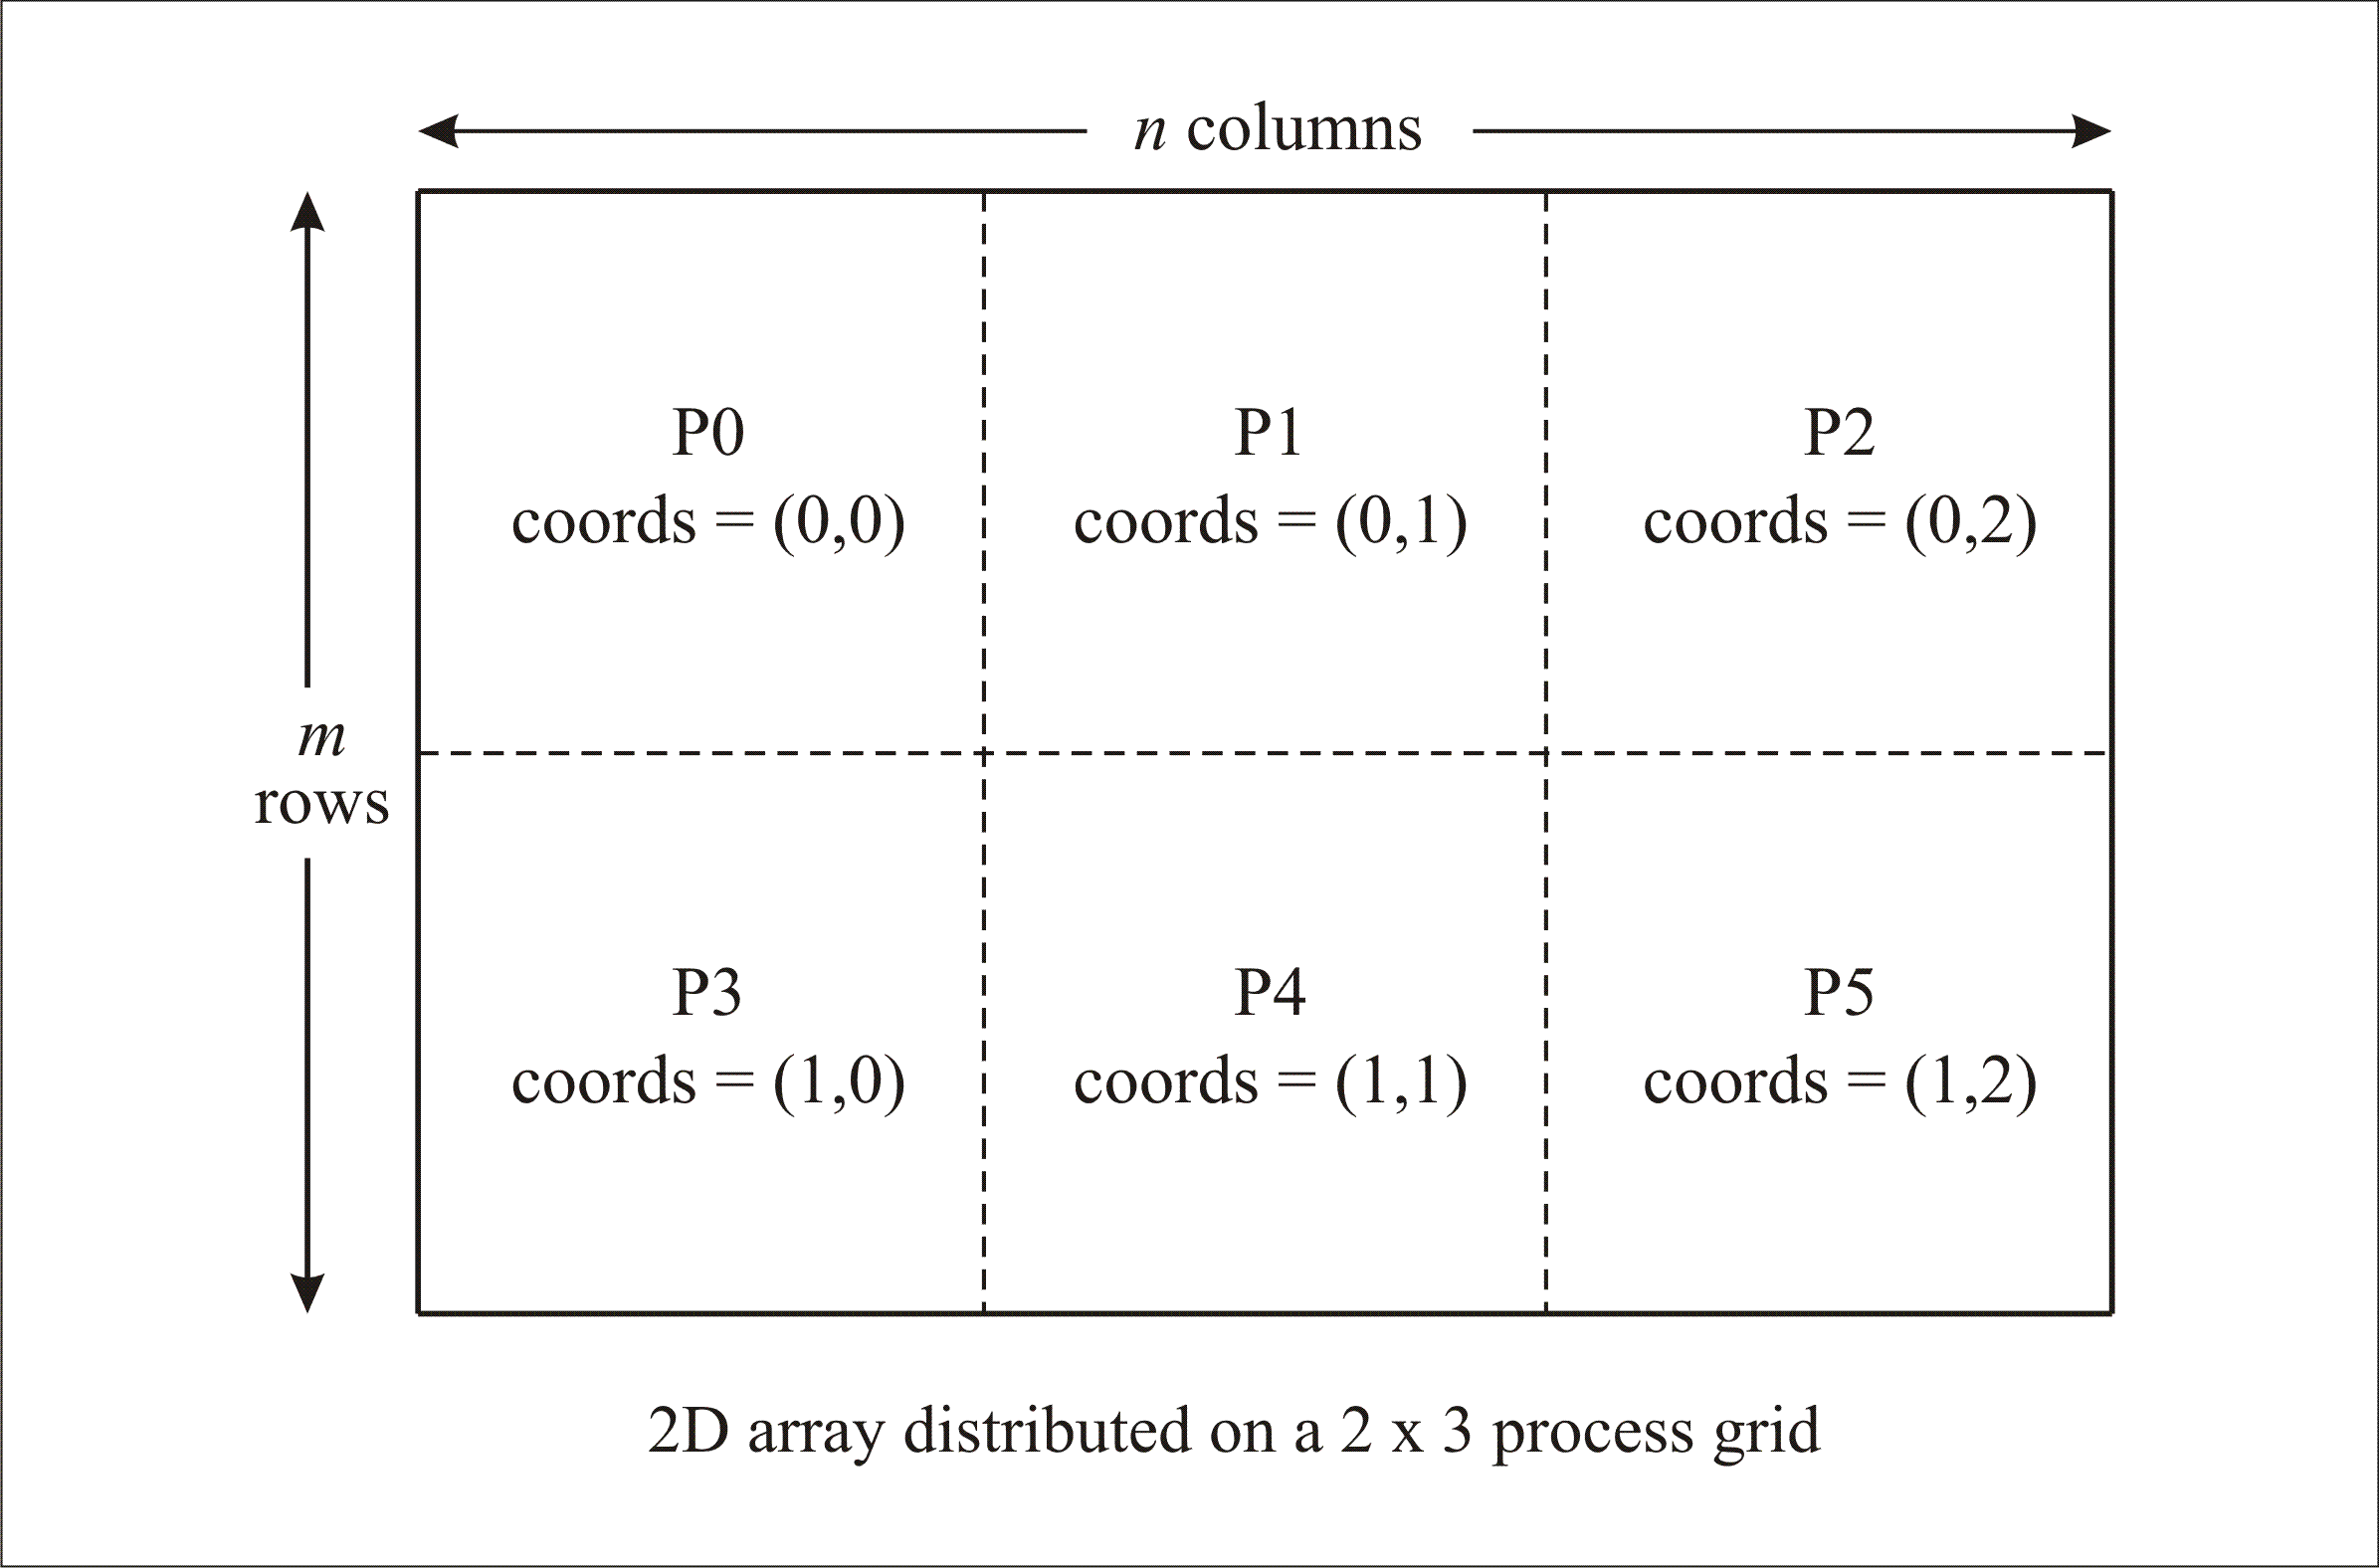
\includegraphics[width=1\textwidth]{slike/darray.png}
  \caption{Подељени низ}
\end{figure}

Осми аргумент функције \texttt{MPI\_Type\_create\_darray} одређује редослед складиштења локалног низа у меморији, као и глобалног низа у фајлу. Девети аргумент је \textit{datatype} који описује ког је типа елемент низа, у овом програму \texttt{MPI\_FLOAT}. Повратна вредност функције је изведени тип података \textit{\&filetype}. После комитовања типа података, нови тип може се користити у постављању погледа(Листинг 3.10). 


\subsection{Неблокирајуће У/И операције и подељене колективне У/И операције}

MPI подржава неблокирајућу верзију независних функција за писање и читање. MPI механизам омогућава ове функције, слично као и неблокирајуће интерпроцесне комуникације. Неблокирајуће функције почињу са 
\texttt{MPI\_File\_ixxx}, нпр.  \texttt{MPI\_File\_iread} и \texttt{MPI\_File\_iwrite\_at}. Неблокирајуће функције враћају \texttt{MPI\_Request} објекат. Могу се користити уобичајене MPI\_Test и MPI\_Wait операције. Користећи ове функције, може доћи до преклапања улазно/излазних операција са осталим комуникацијама у програму. Ова преклапања зависе од квалитета имплементације. За колективне операције, MPI подржава 
ограничен облик неблокирајућих операција, које се називају подељеним колективним У/И операцијама. Да би се користиле подељене колективне функције, корисник мора позвати \zn почетак" функције (\texttt{MPI\_File\_read\_all\_begin}) да би се покренула колективна У/И, као и "крај" функције (\texttt{MPI\_File\_read\_all\_end}) да би се она завршила. Ограничење је да корисник у исто време може имати само једну подељену колективну операцију над једним фајлом. Подељене колективне функције не враћају \texttt{MPI\_Request} објекат.

\subsection{Подељени фајл показивачи}

Постоји три начина да се одреди локација у фајлу са које је потребно прочитати или уписати податке: појединачни фајл показивачи, експлицитна одступања и подељени фајл показивачи.
\textbf{Подељени фајл показивач} је фајл показивач чија вредност је подељена између процеса који се налазе у комуникатору функције \texttt{MPI\_File\_open}. MPI пружа функције \texttt{MPI\_File\_read\_shared} и \texttt{MPI\_File\_write\_shared} које читају/уписују податке са почетком у тренутној локацији подељеног фајл показивача. После позивања ових функција, подељени фајл показивач биће освежен новом количином података који су уписани или прочитани. Следећи позив ових функција ће радити са освеженим подељеним фајл показивачем. Процес може експлицитно померити показивач у \textit{etypes} јединици помоћу функције \texttt{MPI\_File\_seek\_shared}. MPI захтева да сви процеси имају исти фајл поглед када користе подељене фајл показиваче. За остала два начина могу се користити различити фајл погледи. 


\section{Даљински приступ меморији}
MPI-2 омогућава да процес директно приступи подацима другог процеса. Ове операције које омогућавају читање и писање тих података називају се \textit{remote memory access} (\gls{RMA}) операције. Главна карактеристика MPI имплементације је слање података између процеса помоћу операција за слање и примање података. 
Треба приметити да MPI-2 не омогућава реални подељени меморијски модел. Даљинске меморијске операције MPI-2 омогућавају велику флексибилност подељене меморије. 
Даљински приступ меморији је пројектован да ради на машинама са дељеном меморијом и на окружењима која немају дељену меморију, као што су мреже радних станица које користе TCP/IP протокол за комуникацију. Њихова главна предност је флексибилност коју нуде у пројектовању алгоритама. Крајњи програми су преносиви кроз све MPI имплементације и биће ефикасни на свим платформама које омогућавају приступ меморији других процеса.

\subsection{Меморијски оквири}

У строгом прослеђивању порука, бафери за слање и примање су одређени MPI типовима података који представљају делове адреса процеса који се шаљу другим процесима у случају слања, или адреса где ће други процеси уписати податке у случају примања. У MPI-2 имплементацији, појам комуникацијске меморије је генерализован на појам оквира за даљински приступ меморији. Сваки процес
може одредити део адресног простора који је доступан другим процесима за писање и читање. Операције писања и читања, које су покренуте од стране другог процеса називају се \textit{get} и \textit{put} операције за даљински приступ меморији(слика 3.6). Трећи тип операција је accumulate. У MPI-2, оквир представља део меморије једног процеса који чини дистрибуиран објекат, који се назива оквирни објекат. Оквирни објекат је направљен од више оквира, од којих се сваки састоји од локалне меморијске области која је изложена другим процесима.

\begin{figure}[h!]
  \centering
      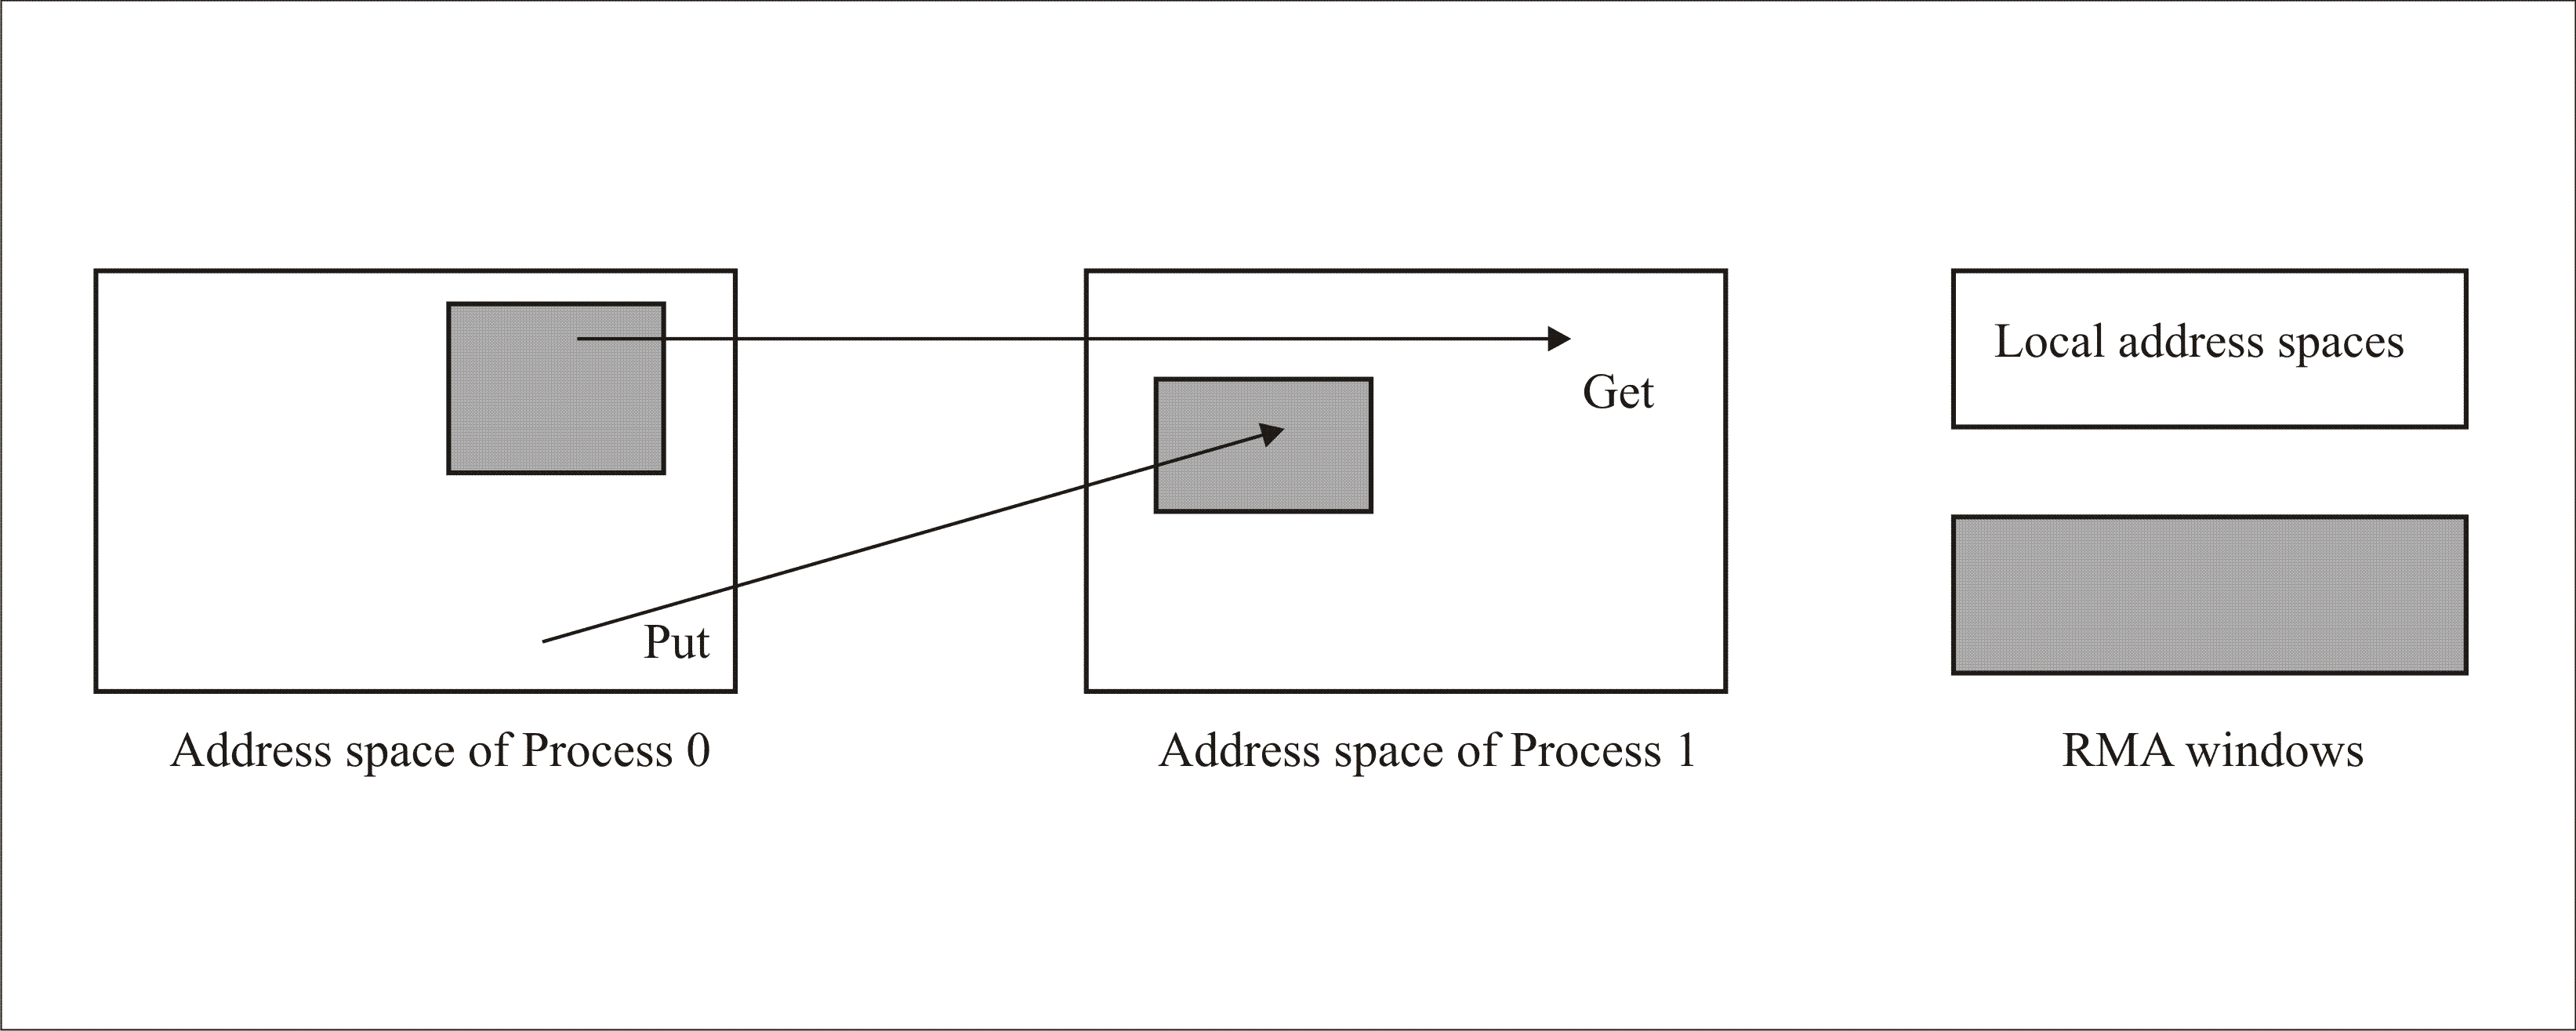
\includegraphics[width=1\textwidth]{slike/mpi_remote.png}
  \caption{Меморијски оквир}
\end{figure}

\subsection{Перформансе програма са даљинским приступом меморији}

Програм за рачунање $\pi$ рачуна вредност броја помоћу нумеричке интеграције. У класичној  верзији постоји 2 типа комуникације. Процес 0 комуницира са корисником и захтева број интервала за интеграцију. Помоћу функције \texttt{MPI\_Bcast} процес 0 шаље тај број другим процесима. Сваки процес затим израчунава парцијалну суму и све суме се сумирају помоћу колективне \texttt{MPI\_Reduce} операције.

У једностраној верзији овог програма, процес 0 снима вредност броја интервала као део RMA оквирног објекта, одакле га други процеси могу једноставно прочитати(Листинг 3.11). После израчунавања парцијалне суме, сви процеси додају своју вредност у други оквирни објекат помоћу accumulate операције. Сваки оквирни објекат садржи само један број у меморији. Оквирни објекти су представљени као променљиве типа \texttt{MPI\_Win}. Функције за креирање оквира су следеће:

\begin{verbatim}
	MPI_Win_create (&n, sizeof(int), 1, MPI_INFO_NULL, MPI_COMM_WORLD, &nwin);
	MPI_Win_create(MPI_BOTTOM, 0, 1, MPI_INFO_NULL, MPI_COMM_WORLD, &nwin);
\end{verbatim}

Позив са процеса 0 треба бити упарен са осталим процесима, иако они не доприносе никакву меморију за оквирни објекат, пошто је \texttt{MPI\_Win\_create} колективна операција над процесима који се налазе у комуникатору. Комуникатор одређује који процеси могу приступити оквирном објекту. Прва два аргумента функције  \texttt{MPI\_Win\_create} су адреса и дужина оквира у бајтовима.

\begin{lstlisting}[style=nonumbers,frame=single,language=C, caption=MPI програм са даљинским приступом меморији]
#include "mpi.h"
#include <math.h>

int main(int argc, char *argv[])
{
	int n, myid, numprocs, i;
	double PI25DT = 3.141592653589793238462643;
	double mypi, pi, h, sum, x;
	MPI_Win nwin, piwin;
	MPI_Init(&argc,&argv);
	MPI_Comm_size(MPI_COMM_WORLD,&numprocs);
	MPI_Comm_rank(MPI_COMM_WORLD,&myid);
	if (myid == 0)
	{
		MPI_Win_create(&n, sizeof(int), 1, MPI_INFO_NULL,
		MPI_COMM_WORLD, &nwin);
		MPI_Win_create(&pi, sizeof(double), 1, MPI_INFO_NULL,
		MPI_COMM_WORLD, &piwin);
	}
	else
	{
		MPI_Win_create(MPI_BOTTOM, 0, 1, MPI_INFO_NULL,
		MPI_COMM_WORLD, &nwin);
		MPI_Win_create(MPI_BOTTOM, 0, 1, MPI_INFO_NULL,
		MPI_COMM_WORLD, &piwin);
	}
	MPI_Win_fence(0, nwin);
	while (1)
	{
		if (myid == 0)
		{
			printf("Enter the number of intervals: (0 quits) ");
			fflush(stdout);
			scanf("%d",&n);
			pi = 0.0;
		}
		MPI_Win_fence(0, nwin);
		if (myid != 0)
		MPI_Get(&n, 1, MPI_INT, 0, 0, 1, MPI_INT, nwin);
		MPI_Win_fence(0, nwin);
		if (n == 0)
		{
			break;
		}
		else
		{
			h = 1.0 / (double) n;
			sum = 0.0;
			for (i = myid + 1; i <= n; i += numprocs)
			{
				x = h * ((double)i - 0.5);
				sum += (4.0 / (1.0 + x*x));
			}
			mypi = h * sum;
			MPI_Win_fence( 0, piwin);
			MPI_Accumulate(&mypi, 1, MPI_DOUBLE, 0, 0, 1, MPI_DOUBLE,
			MPI_SUM, piwin);
			MPI_Win_fence(0, piwin);
			if (myid == 0)
			printf("pi is approximately %. 16f, Error is %. 16f/n",
			pi, fabs(pi - PI25DT));
		}
	}
	MPI_Win_free(&nwin);
	MPI_Win_free(&piwin);
	MPI_Finalize();
	return 0;
}
\end{lstlisting}

Следећи аргумент је displacement unit који се користи да одреди одступање локације у меморији. Сваки оквирни објекат садржи једну променљиву, код којих је одступање нула, тако да одступање у овом примеру може да се занемари. Четврти аргумент је \texttt{MPI\_Info} који се може користити да побољша учинак RMA операција. Пети аргумент је комуникатор који одређује скуп процеса који ће имати приступ меморији оквирног објекта. MPI имплементација враћа \texttt{MPI\_Win} објекат као последњи аргумент. После позива функције \texttt{MPI\_Win\_create}, сваки процес који се налази у комуникатору има приступ
података \textit{nwin} помоћу операција \textit{put}, \textit{get} и \textit{accumulate}. За меморију оквира није потребно алоцирати посебну меморију, већ се користи меморија самог процеса, којој остали процеси приступају.  
MPI имплементација омогућава алоцирање посебне меморије позивом функције \texttt{MPI\_Alloc\_mem}.

Други позив функције \texttt{MPI\_Win\_create} креира оквирни објекат piwin дозвољавајући сваком процесу да приступи променљивој $\pi$ првог процеса, где ће бити смештена израчуната вредност броја $\pi$.
У следећем делу програма, процес са рангом 0 захтева број интервала, а затим остали процеси рачунају број $\pi$. Петља се завршава када корисник унесе нулу. Процеси којима ранг није нула, вредност броја $n$ узимају  директно из оквирног објекта без икакве додатне акције. Пре позива функције MPI\_Get или било које функције за даљински приступ меморији, потребно је позвати функцију \texttt{MPI\_Win\_fence} да одвоји операције. MPI имплентација омогућава специјални механизам синхронизације за операције дељене меморије - \textit{three of them}. \textit{Fence} операција је изазвана функцијом \texttt{MPI\_Win\_fence }која захтева два аргумента. Први аргумент је потврдни аргумент за дозвољавање оптимизације. Увек исправан потврдни аргумент је 0. Други аргумент је оквир на коме се операција извршава. \texttt{MPI\_Win\_fence} се може тумачити као баријера која одваја локалне операције на оквиру од скупа даљинских операција на оквиру.

У овом програму одваја читање вредности променљиве $n$ од осталих даљинских операција које следе. Вредност променљиве $n$ остали процеси добијају помоћу позивом:

\begin{verbatim}
MPI_Get(&n, 1, MPI_INT, 0, 0, 1, MPI_INT, nwin)
\end{verbatim}

Аргументи ове функције су слични аргументима функција које примају или шаљу податак. Get операција је слична операцији примања, па су зато прва три аргумента опис податка који се прима (адреса, количина и тип податка).  Следећи аргумент је ранг процеса чијој меморији приступамо. У овом случају је ранг 0, јер сви процеси приступају меморији првог процеса.
Следећа три аргумента дефинишу бафер за слање (адреса, количина и тип податка). Овде се адреса даје као одступање од почетка локације у дељеној меморији. У овом случају је 0, зато што се приступа само једној вредности. Последњи аргумент је објекат оквира.  \texttt{MPI\_Get} је неблокирајућа операција. После позива ове функције не може се гарантовати да је вредност смештена у променљивој $n$. Зато је потребно позвати \texttt{MPI\_Win\_fence}. Сваки процес рачуна свој део суме $mypi$. Сада се позива \texttt{MPI\_Win\_fence}, али на оквирном објекту piwin, како би се покренуо други 
RMA приступ. Позивом функције \texttt{MPI\_Accumulate}, сабирају се све суме процеса у глобалну суму.

\begin{verbatim}
MPI_Accumulate(&mypi, 1, MPI_DOUBLE, 0, 0, 1, MPI_DOUBLE, MPI_SUM, piwin)
\end{verbatim}

Прва три аргумента одређују локалну променљиву (адреса, количина и тип податка), док је четврти аргумент ранг процеса. Следећа три аргумента описују променљиву коју је потребно изменити.
Аргумент који следи је операција коју је потребно извршити. Пошто нам је потребна глобална сума, у овом случају то је \texttt{MPI\_SUM}. Последњи аргумент је објекат оквира.
Програм се завршава штампањем вредности броја $\pi$ и ослобађањем меморије објекта помоћу функције  \texttt{MPI\_Win\_free}.  \texttt{MPI\_Win\_free} је колективна функција над комуникатором прослеђеног објекта оквира.


Неке MPI функције у програмском језику C дате су у Листингу 3.12:

\begin{lstlisting}[style=nonumbers,frame=single,language=C, caption= MPI функције]
int MPI_Win_create(void *base, MPI_Aint size, int disp_unit, MPI_Info info,MPI_Comm comm, MPI_Win *win)
int MPI_Win_fence(int assert, MPI_Win win)
int MPI_Get(void *origin_addr, int origin_count, MPI_Datatype origin_datatype,
int target_rank, MPI_Aint target_disp, int target_count,
MPI_Datatype target_datatype, MPI_Win win)
int MPI_Accumulate(void *origin_addr, int origin_count,
MPI_Datatype origin_datatype, int target_rank,
MPI_Aint target_disp, int target_count,
MPI_Datatype target_datatype, MPI_Op op, MPI_Win win)
int MPI_Win_free(MPI_Win *win)
\end{lstlisting}


\section{Управљање процесима}
Процес модел који се користи у MPI-1 имплементацијама користи фиксиран број процеса током MPI рачунања. Ово је концептуално једноставан модел, јер ставља све сложености интеракције са оперативним системом (који мора бити 
укључен у стварање процеса) потпуно изван оквира апликације. Када се изврши \texttt{MPI\_Init}, процеси су покренути и комуникатор \texttt{MPI\_COMM\_WORLD} има коначан број процеса. Они могу међусобно да комуницирају преко комуникатора. Други комуникатори имају своје групе, која је подгрупа \texttt{MPI\_COMM\_WORLD} комуникатора. Динамичнији приступ управљањем процеса пролазилази из \gls{PVM} (\textit{Parallel Virtual Machine}) заједнице, где се процеси покрећу под контролом апликације. Интеркомуникатор служи да повеже две групе процеса. Интеркомуникатори омогућавају природан начин да опишу \textit{spawning} процесе. Интеркомуникатори се могу спојити помоћу функције MPI\_Intercomm\_merge, чије је повратна вредност нови интракомуникатор.

\subsection{\textit{Spawning} процеса}
У MPI-2 имплементацијама, процес се креира помоћу функције \texttt{MPI\_Comm\_spawn}. Кључна предности \texttt{MPI\_Comm\_spawn} су:

\begin{itemize}
	\item Ово је колективна операција над новим процесима.
	\item Нови процеси имају свој властити \texttt{MPI\_COMM\_WORLD}.
	\item Функција \texttt{MPI\_Comm\_parent}, позвана од стране детета процеса, као повратну вредност има интеркомуникатор који садржи децу процеса као локалну групу и родитеље као даљинску групу.
\end{itemize}

\subsection{Пример паралелног копирања}

Једноставан услужни програм који извршава паралелно копирање тако што копира фајл са локалног диска машине на локалне дискове других машина(Листинг 3.13). Са MPI имплементацијом може се на скалабилан начин смањити време извршавања програма. Основни начин слања фајла помоћу MPI-а је користећи функцију  \texttt{MPI\_Bcast} за слање са \textit{root} процеса(слика 3.7). Да би се покренуо програм, потребно је на свакој машини имати извршни фајл. 

\begin{figure}[h!]
  \centering
      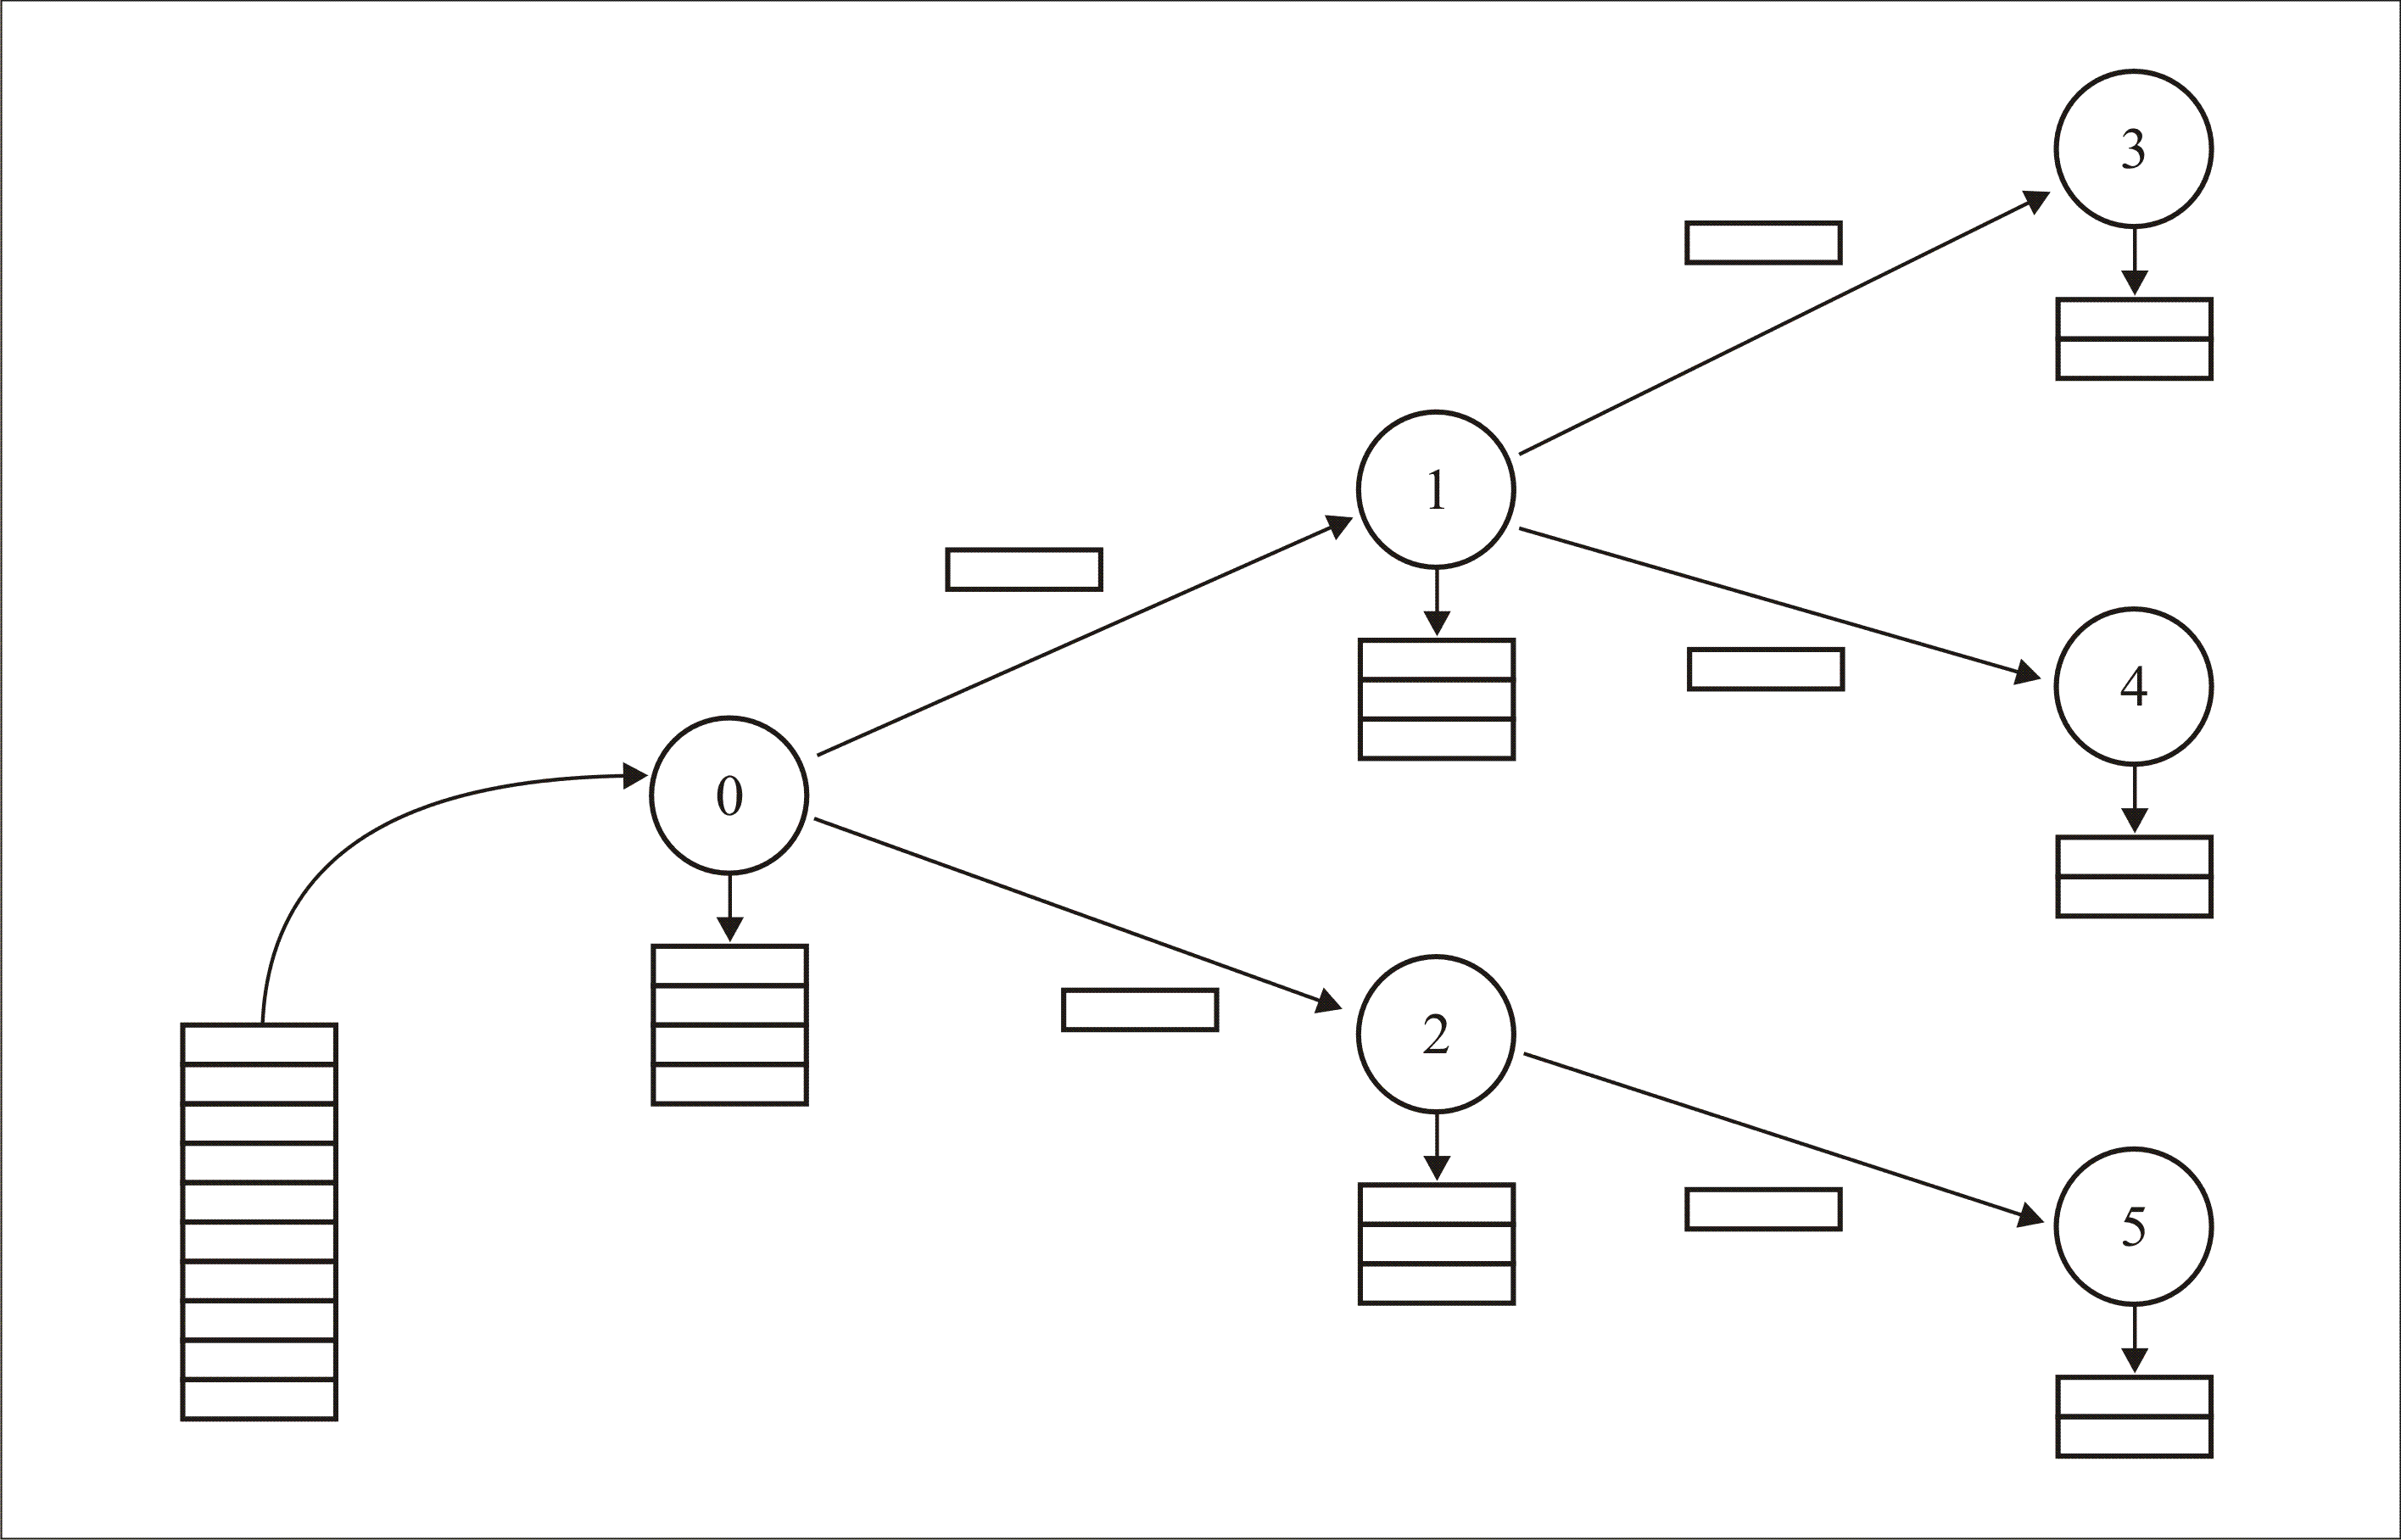
\includegraphics[width=0.5\textwidth]{slike/bcast.png}
  \caption{MPI remote}
\end{figure}

Процес са рангом 0 чита фајл, а затим користећи \texttt{MPI\_Bcast} шаље блок по блок фајла другим процесима. Овај начин садржи 3 облика паралелизма:

\begin{itemize}
	\item Сви процеси извршавају паралелне улазно/излазне операције са фајлом.
	\item Већи део слања порука између процеса се одвија паралелно.
	\item Подела фајла у блокове се одвија у \textit{pipeline} паралелизму.
\end{itemize}

Први део програма је парсирање листе свих машина на које је потребно ископирати фајл, а затим и креирање празног фајла на тим машинама. Функција makehostlist парсира први аргумент и штампа списак машина у фајл чији је назив прослеђен као други аргумент. Број машина је повратна вредност ове функције. 

\begin{verbatim}
makehostlist( argv[1], "targets", &num_hosts );
\end{verbatim}

Да би сви процеси знали име фајла у коме се налази списак машина, потребно је да се назив фајла проследи функцији која покреће нове процесе \texttt{MPI\_Comm\_spawn} помоћу инфо објекта. Креира се инфо објекат који садржи \zn targets" као вредност резервисаног кључа. Овај инфо кључ једноставно говори функцији \texttt{MPI\_Comm\_spawn} да погледа фајл  \zn targets" за више информација. 

\begin{lstlisting}[style=nonumbers,frame=single,language=C, caption= MPI програм за паралелно копирање]
#include "mpi.h"
#include <stdio.h>
#include <sys/types.h>
#include <sys/stat.h>
#include <fcntl.h>
#define BUFSIZE 256*1024
#define CMDSIZE 80

int main( int argc, char *argv[] )
{
	int	num_hosts, mystatus, allstatus, done, numread;
	int	infd, outfd;
	char utfilename[MAXPATHLEN], controlmsg[CMDSIZE];
	char buf[BUFSIZE];
	char soft_limit[20];
	MPI_Info hostinfo;
	MPI_Comm pcpslaves, all_processes;
	MPI_Init( &argc, &argv );
	makehostlist( argv[1], "targets", &num_hosts );
	MPI_Info_create( &hostinfo );
	MPI_Info_set( hostinfo, "file", "targets" );
	sprintf( soft_limit, "0:%d", num_hosts );
	MPI_Info_set( hostinfo, "soft", soft_limit );
	MPI_Comm_spawn( "pcp_slave", MPI_ARGV_NULL, num_hosts,
	hostinfo, 0, MPI_COMM_SELF, &pcpslaves,
	MPI_ERRCODES_IGNORE );
	MPI_Info_free( &hostinfo );
	MPI_Intercomm_merge( pcpslaves, 0, &all-processes );
	strcpy( outfilename, argv[3] );
	if ( (infd = open( argv[2], O_RDONLY ) ) == -1 )
	{
		fprintf( stderr, "input %s does not exist\n", argv[2] );
		sprintf( controlmsg, "exit" );
		MPI_Bcast( controlmsg, CMDSIZE, MPI_CHAR, 0, all_processes );
		MPI_Finalize();
		return -1 ;
	}
	else
	{
		sprintf( controlmsg, "ready" );
		MPI_Bcast( controlmsg, CMDSIZE, MPI_CHAR, 0, all_processes );
	}
	MPI_Bcast( outfilename, MAXPATHLEN, MPI_CHAR, 0,
	all_processes );
	if ( (outfd = open( outfilename, O_CREAT|O_WRONLY|O_TRUNC,
	S_IRWXU ) ) == -1 )
	{
		mystatus = -1;
	}
	else
	{
		mystatus = 0;
	}
	MPI_Allreduce( &mystatus, &allstatus, 1, MPI_INT, MPI_MIN,
	all_processes );
	if ( allstatus == -1 )
	{
		fprintf( stderr, "Output file %s could not be opened\n",
		outfilename );
		MPI_Finalize();
		return 1 ;
	}
	/* at this point all files have been successfully opened */
	done = 0;
	while (!done) 
	{
		numread = read( infd, buf, BUFSIZE );
		MPI_Bcast( &numread, 1, MPI_INT, 0, all_processes );
		if ( numread > 0 ) 
		{
			MPI_Bcast( buf, numread, MPI_BYTE, 0, all_processes );
			write( outfd, buf, numread );
		}
		else
		{
			close( outfd );
			done = 1;
		}
	}
	MPI_Comm_free( &pcpslaves );
	MPI_Comm_free( &all_processes );
	MPI_Finalize();
	return 0;
}
\end{lstlisting}

Програм конвертује интеркомуникатор \texttt{pcpslaves} који садржи покренут процес и процесе које је креирала функција \texttt{MPI\_Comm\_spawn} у један заједнички интракомуникатор помоћу \texttt{MPI\_Intercomm\_merge}. Интракомуникатор \textit{all\_processes} се користи као комуникатор између \textit{root} машине и осталих машина. Процеси покушавају отворити улазни фајл, и уколико дође до грешке, шаље се сигнал за прекид рада.

Да би се знало да је сваки процес отворио фајл, користи се \texttt{MPI\_Allreduce} функција са \texttt{MPI\_MIN} операцијом. Уколико било који процес не може да отвори фајл, сви процеси ће то сазнати и позвати 
\texttt{MPI\_Finalize} за прекид рада. Код за дете процес је сличан коду родитеља процеса, с тим што дете процеса мора да позове \texttt{MPI\_Comm\_get\_parent} функцију да успостави контакт са родитељем. Дете процес не обрађује аргументе нити штампа поруке. Родитељ процес затим чита блок по блок фајла и шаље осталим процесима. На крају сви процеси ослобађају интеркомуникатор креиран од стране  \texttt{MPI\_Comm\_spawn} и обједињени интракомуникатор. Главна разлика између \texttt{MPI\_Comm\_spawn} функције и осталих  система за слање порука је природност колективних операција. У MPI имплементацији, група процеса колективно креира другу групу процеса који су међусобно синхронизовани. Тиме се спречавају додатни услови и омогућава неопходна комуникациона инфраструктура.

\chapter{Закључак}     

 Главни недостатак \textit{Lustre} фајл система је компликована инсталација у односу на његову алтернативу NFS. Међутим, уштеда времена у току вршења тестирања је огромна што се никако не сме занемарити. Та предност је нарочито значајна при извршавању обимних математичких операција које захтевају рад са фајловима. MPI-2 стандард са новим функцијама које омогућавају паралелне улазно/излазне операције заједно са \textit{Lustre} фајл системом чине најбољу комбинацију за паралелне програме. Обзиром да је \textit{Lustre} фајл систем доступан бесплатно, да је његов опоравак лакши у случају отказивања чврстог диска и да подржава паралелне операције са фајловима, треба му се дати апсолутна предност у односу на NFS. Једина алтернатива коју \textit{Lustre} тренутно има на тржишту је \textit{PanFS} компаније \textit{Panasas}, који се нешто лакше конфигурише и администрира, али по цену затворености кода и више цене. 


\chapter{Тестирање брзине извршавања У/И операција}

Како би се увидела предност \textit{Lustre} фајл система у односу на NFS фајл систем, вршено је мерење брзине извршавања У/И операција на \textit{Мedflow} кластеру високих перформанси који користи оба наведена фајл система. Тестирање је вршено помоћу три различите апликације:


\begin{itemize}
\item \textit{Iozone} - апликација намењена тестирању перформанси улазно-излазних операција,
\item \texttt{dd} - једноставан UNIX системски алат за конверзију и копирање фајлова,
\item \textit{Game of Life} - "реална" апликација која поред У/И операција поседује и делове у којима се интензивно рачуна.
\end{itemize}

\section{Хардверска конфигурација кластера}

Medflow кластер је састављен од HP Proliant SL230s Gen8 и HP Proliant SL250s Gen8 радних чворова, заснованих на Intel® Xeon® E5-2600 (Sandy Bridge) процесорима. Кластер се састоји од следећих компоненти:

\begin{itemize}

\item 18 радних чворова HP Proliant SL230s Gen8 са 2 Intel® Xeon® E5-2660 процесора (2.2GHz – 8 cores - 20MB L3 cache - 95W) и  64GB RAM меморије.
\item 4 радна чвора P Proliant SL250s са 2 Intel® Xeon® E5-2670 (2.6GHz – 8 cores - 20MB L3 cache - 115W) процесора и  64GB RAM меморије. Сваки од ових чворова садржи и 1 GPU NVIDIA Tesla
M2090 6G графичку картицу.
\item Једног \textit{Mellanox Infiniband} QDR свич преко кога су повезани чворови.  
\item Једног управљачког сервера DL380pGen8 који омогућава пријаву на систем.
\item Једног управљачког сервера DL380pGen8 који омогућава функционисање паралелног фајл система.
\item Система за складиштење података који садржи 1 \textit{HP P2000 G3 Modular Smart Array System} повезан на управљачки сервер, што даје укупно 12TB простора (6 HDD дискова по 2TB). Низ је конфигурисан као RAID ниво 6. Сви чворови могу приступити овим дисковима помоћу \textit{Lustre} протокола.
\end{itemize}
 
 \begin{figure}[h!]
   \centering
       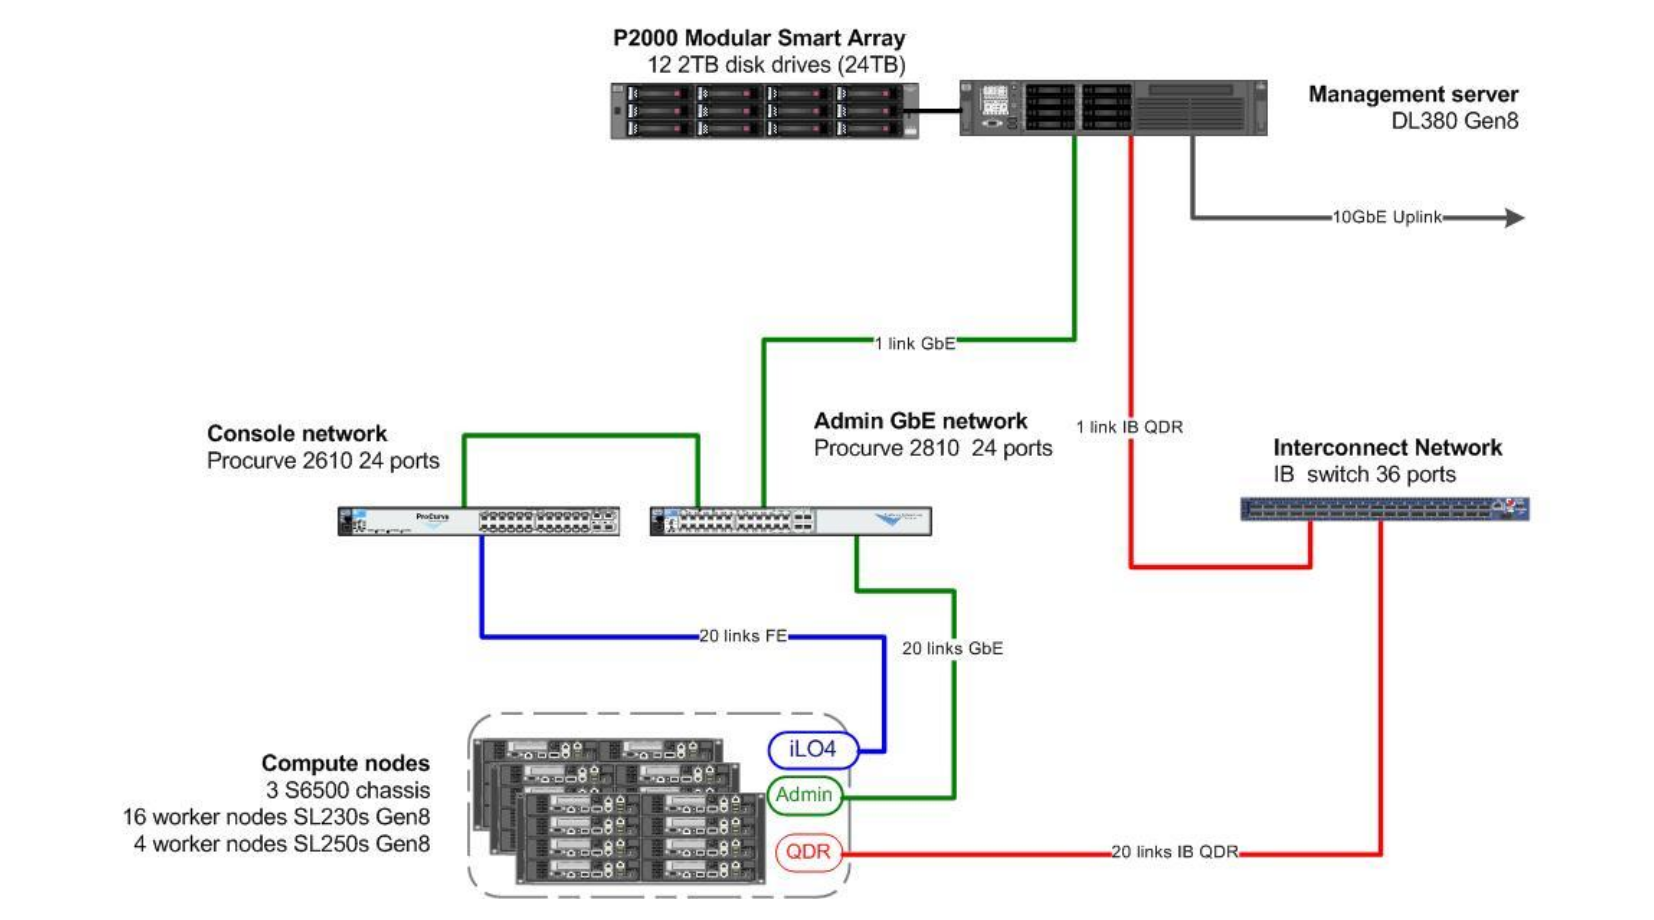
\includegraphics[width=1\textwidth]{slike/medflow.png}\\[1cm]
   \caption{Компоненте кластера}
 \end{figure}
 
Кластер је конфигурисан са Linux Kernel 2.6 на свим чворовима. Scientific Linux 6.6 64-bit је инсталиран како на управљачком чвору, тако и на радним чворовима. Ресурсима кластера се управља помоћу \textit{TORQUE} и \textit{Maui} сервиса. Први је намењен контроли и управљању кластер пословима, док је други распоређивач. 
 
Програмско окружење је засновано на OpenMPI библиотекама за Linux оперативни систем. На кластеру је инсталирана OpenMPI верзија 1.6.5. Треба нагласити и да је NFS фајл систем инсталиран постављен само на једном диску, док Lustre користи цео RAID6 низ. 

\section{Iozone тестирање}
\textit{Iozone} је алат за мерење брзине У/И операција фајл система. Он генерише и мери трајање великог броја операција са фајловима. \textit{Iozone} може бити  инсталиран на великом броју архитектура и такође може радити у оквиру многих оперативних система. Тестирање се врши кроз следеће операције:

\begin{itemize}
\item \textit{Write} - мери брзину уписа података у нови фајл.
\item \textit{Re-write} - мери брзину уписа у фајл који већ постоји
\item \textit{Read} - мери брзину читања из фајла
\item \textit{Re-read} - мери брзину читања из фајла који је претходно прочитан
\item \textit{Random read} - мери брзину читања из фајла са насумичним приступом локацијама унутар фајла
\item \textit{Random write} - мери брзину писања у фајл са насумичним приступом локацијама унутар фајла
\item \textit{Random mix} - мери брзину писања и читања из фајла са насумичним приступом локацијама унутар фајла
\item \textit{Backwards read} - мери брзину читања из фајла уназад
\item \textit{Record rewrite} - мери брзину писања података у одређени део фајла
\item \textit{Strided read} - мери брзину читања из фајла са тачно одређеним параметрима
\item \textit{Fwrite} - мери брзину писања у фајл помоћу функције \texttt{fwrite()}
\item \textit{Fread} - мери брзину читања из фајла помоћу функције \texttt{fread()}
\item \textit{Freread} - мери поновно читања из фајла  помоћу функције \texttt{fwrite()}
\end{itemize}


\subsection{Инсталација и покретање програма}

\textit{Iozone} програм се инсталира помоћу следећих команди:
\begin{lstlisting}[style=nonumbers,frame=single,language=C, caption= Инсталација Iozone]
wget http://www.iozone.org/src/current/iozone3_394.tar

tar xvf iozone3_394.tar 

cd iozone3_394/src/current

make

make linux

\end{lstlisting}

Овај програм је могуће покренути и помоћу великог број параметара. Конкретни параметри који су коришћени за тестирање на кластеру имају следеће значење:

\begin{itemize}
\item \texttt{-b назив фајла} - генерисање Excel излазног фајла
\item \texttt{-c} - мери и време које је потребно за функцију \textit{ close()}
\item \texttt{-I} - користи \textit{DIRECT I/O} заставицу за све фајл операције
\item \texttt{-о} - уписује синхроно на диск. \textit{Iozone} отвара фајл са \textit{O\_SYNC} заставицом
\item \texttt{-r} - oдређује величину записа у килобајтима
\item \texttt{-s} - oдређује величину фајла који се користи за тестирање 
\end{itemize}
Програм се покреће помоћу команде:
\begin{verbatim}
./iozone -s 25000000 -r 1024 -I -c -o -b output.xls
\end{verbatim}

Резултати програма се могу видети у фајлу \textit{output.xls}.

  \begin{figure}[h!]
    \centering
        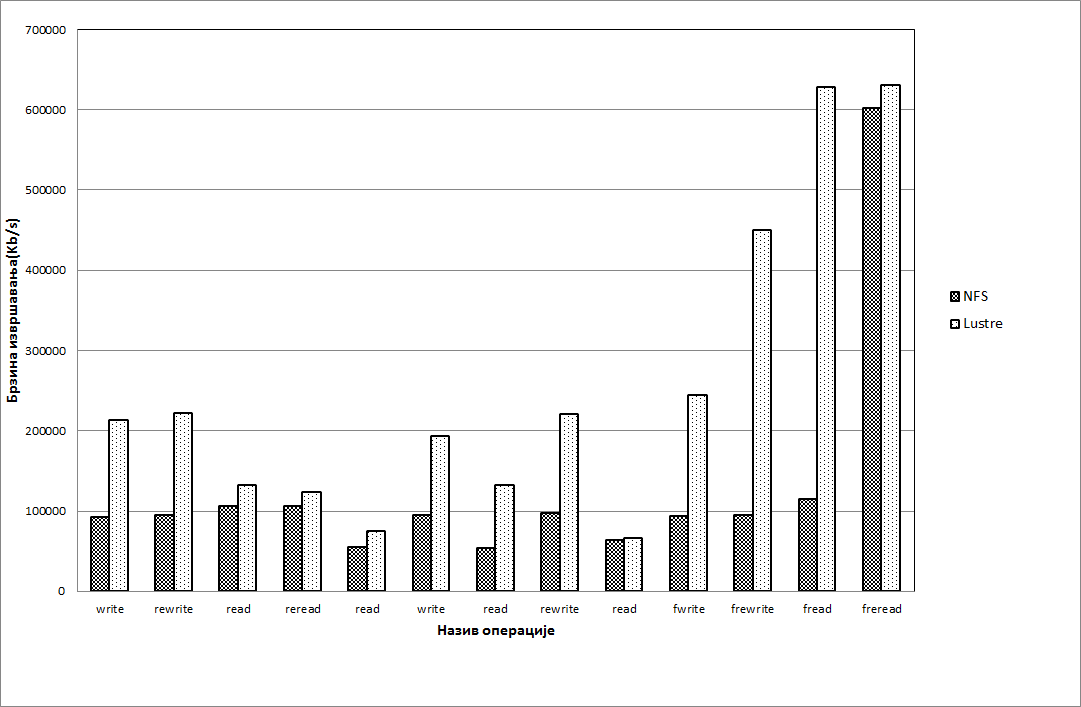
\includegraphics[width=0.85\textwidth]{slike/results/iozone.png}\\[1cm]
    \caption{\textit{Iozone} резултати}
  \end{figure}
  
Посматрајући резултате представљене на Слици 4.2, закључујемо да је брзина извршавања улазно/излазних операција \textit{Lustre} фајл система значајно већа у односу на брзину NFS система без обзира на врсту операције која се извршава. Највећа разлика у брзини се уочава код теста који користи \texttt{fread()} команду, док је најмања разлика у брзини при извршавању операције обичног читања.
  
\section{Тестирање помоћу \texttt{dd} програма }

\texttt{dd} је једноставан алат који служи за писање и читање блокова података диска. Он такође мери и брзину којом је операција извршена.

Параметри командне линије су:

\begin{itemize}
\item \texttt{if} - улазни фајл
\item \texttt{of} - излазни фајл
\item \texttt{bs} - величина блока
\item \texttt{count} - број блокова
\end{itemize}
Програм за упис у фајл  се покреће командом:
\begin{verbatim}
dd if=/dev/zero bs=1M count=16384 of=file_16GB
\end{verbatim}
а за читање из фајла:
\begin{verbatim}
dd if=file_16GB bs=1M of=/dev/null
\end{verbatim}
Добијени су следећи резултати:
\begin{figure}[H]
   \centering
       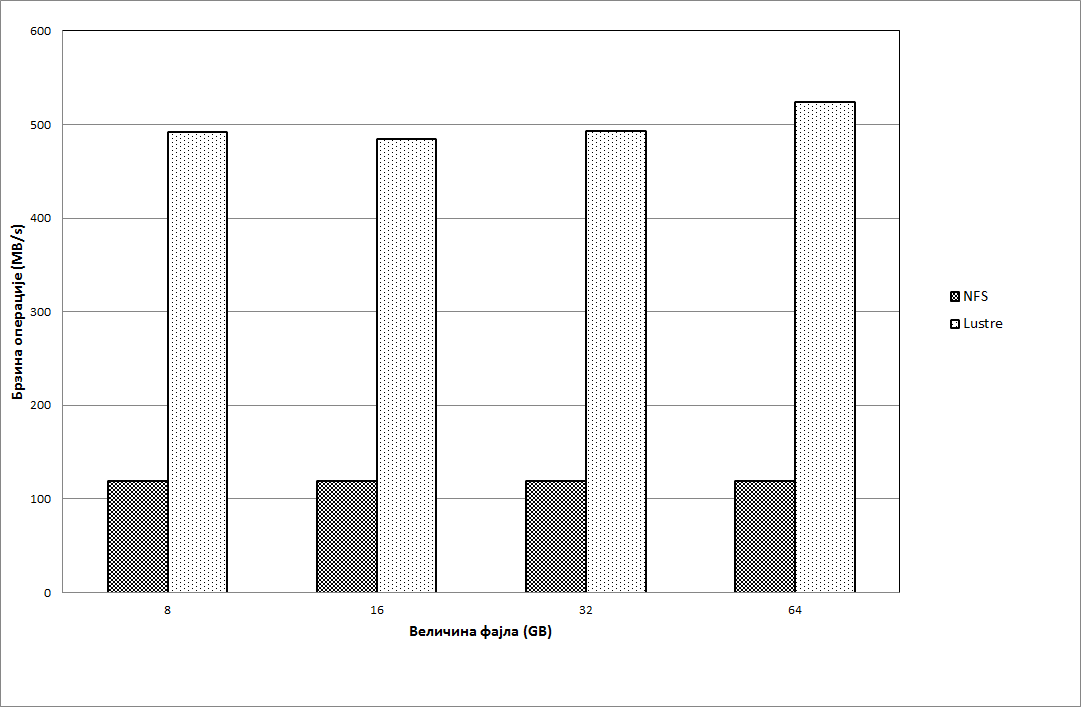
\includegraphics[width=0.85\textwidth]{slike/results/dd_read_speed.png}\\[1cm]
   \caption{Резултати брзине читања}
\end{figure} 
\begin{figure}[H]
    \centering
        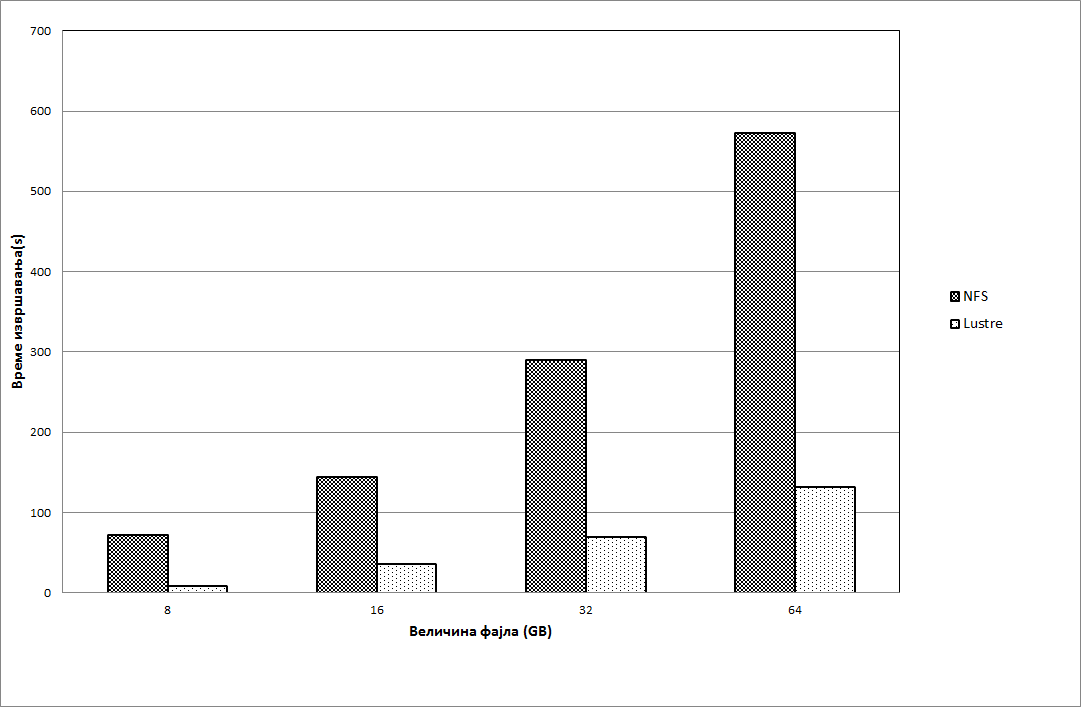
\includegraphics[width=0.85\textwidth]{slike/results/dd_read_time.png}\\[1cm]
    \caption{Резултати времена извршавања програма читања}
\end{figure}  
\begin{figure}[H]
     \centering
         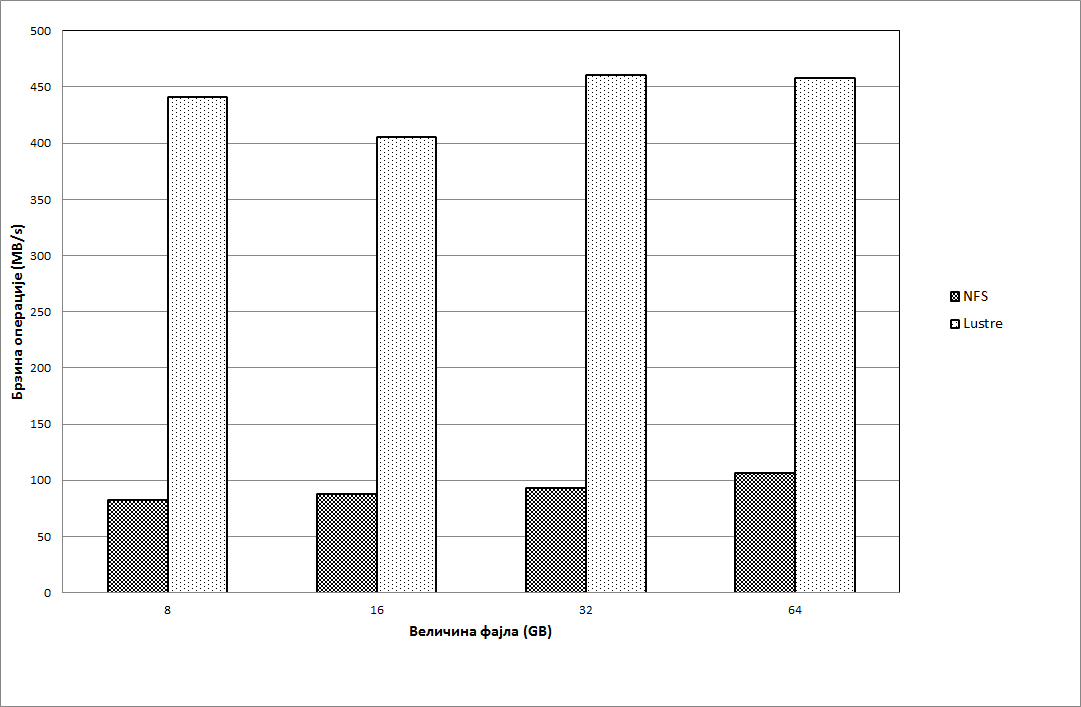
\includegraphics[width=0.85\textwidth]{slike/results/dd_write_speed.png}\\[1cm]
     \caption{Резултати брзине писања}
\end{figure}   
\begin{figure}[H]
      \centering
          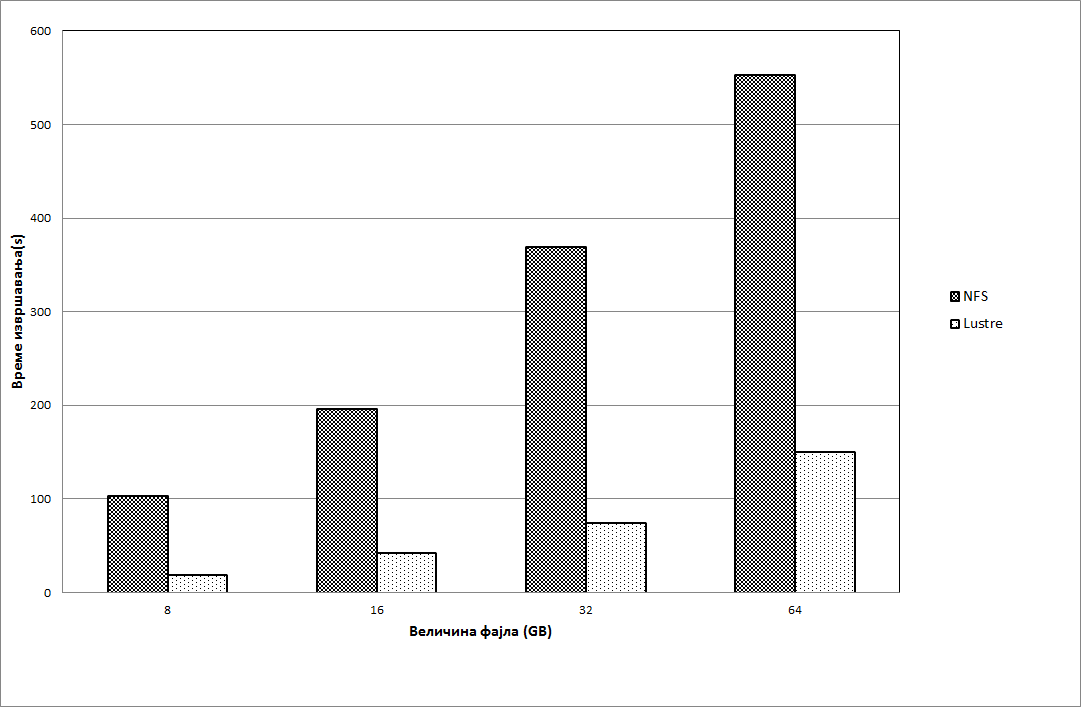
\includegraphics[width=0.85\textwidth]{slike/results/dd_write_time.png}\\[1cm]
      \caption{Резултати времена извршавања програма писања}
\end{figure}   
 
Анализирајући слике 4.3 и 4.5 на којима је приказана брзина читања односно писања закључује се да је \textit{Lustre} фајл систем вишеструко бржи независно од величине фајла који се чита, односно који се уписује.
На сликама 4.4 и 4.6, које приказују време извршавања програма читања, односно писања, уочава се да је разлика у овим фајл системима већа уколико је величина фајла већа. Што је фајл већи, \textit{Lustre} показује већу супериорност у односу на NFS.

\section{Game of Life}
\textit{Game of Life} је најпознатији пример ћелијског аутомата који је осмислио британски математичар Џон Конвеј 1970 године. Ова игра је игра без играча, што значи да је њена еволуција одређена првобитним стањем. 
За тестирање је коришћен \textit{Game of life} MPI-2 програм, коме су дадате функције читања и уписа стања ћелија, које се позивају након сваког корака симулације. Програм је покретан на \textit{Lustre} фајл систему, а затим са истим улазним параметрима на NFS фајл систему. \textit{Game of Life} је погодан јер не захтева додатне корисничке уносе након покретања програма. Матрицa помоћу којe сe прате стања ћелија могуће је декомпоновати независно од броја процеса. Подешавајући улазне параметре, мења се и величина података коју је потребно уписати у фајл.

\subsection{Правила}
\textit{Game of Life} је представљена бесконачном дводимензионалном мрежом квадратних ћелија од којих је свака у једном од два могућа стања: активном или пасивном. Свака ћелија је у односу са осам суседних ћелија, које су са њом повезане хоризонтално, вертикално или дијагонално. Са сваким кораком у времену јављају се следеће транзиције:

\begin{itemize}
\item Било која активна ћелија која има мање од две активне ћелије које су јој суседне постаје пасивна.
\item Било која жива ћелија са више од три активне ћелије које су јој суседне постаје пасивна да не би дошло до пренатрпаности.
\item Било која ћелија са две или три активне суседне ћелије живи, не мења се и преноси на следећу генерацију.
\item Било која пасивна ћелија која има три активне суседне ћелије постаће и сама активна.
\end{itemize}

Почетни модел представља почетну популацију система. Свака популација је чиста функција претходне. Правило се наставља примењивати узастопно ради креирања наредних генерација.

\subsection{Порекло}
Конвеј је био заинтересован за проблем представљен четрдесетих година двадесетог века од стране реномираног математичара Џон ван Нојмана који је покушавао да пронађе машину која би могла да изради копије себе и успео је када је пронашао математички модел за такву машину са веома компликованим правилима на правоугаоној мрежи. Игра је доживела своје прво јавно појављивање у октобру 1970-е у колумни „Математичке игре“ под називом фантастичне комбинације Џона Конвеја. Са теоретске тачке гледишта је занимљиво, јер има моћ универзалне Тјурингове машине. Све што се може алгоритамски обрачунавати може се израчунати и са Конвејевом \textit{Game of Life}.

Још од њеног објављивања, \textit{Game of Life} је привукла велико интересовање због изненађујућих начина на који се обрасци могу развијати. Занимљиво је за физичаре, биологе, економисте, математичаре, филозофе, научнике и остале да посматрају начин на који се сложени обрасци могу појавити из примене веома једноставних правила. На пример, филозоф и научник Даниел Ц. Денет је користио Конвејеве \textit{Game of Life}  интензивно да илуструје могућу еволуцију сложених филозофских конструкција, као што су свест и слободна воља, од релативно једноставног скупа детерминистичких физичких закона који регулишу наш сопствени универзум.
Популарност Конвејеве игре је потпомогнута њеном појавом баш у време појаве нове генерације јефтиних мини рачунара који су пуштени у промет. Игра може да се активира ноћу, током сати када су машине иначе неискоришћене. За многе, \textit{Game of Life} је једноставно програмирање, изазов, забаван начин да губимо циклусе процесора. За неке, међутим, \textit{Game of Life} је више филозофске конотације.

\section{Опис програма}
Програм је написан у C програмском језику користећи MPI функције. На почетку програма се учитавају параметри програма. 

Улазни параметри програма су:
\begin{itemize}
\item начин генерисања почетне популације 
\item број процеса
\item величина квадратне матрице
\item број итерација
\item начин уписа - уколико је 0 онда се матрица уписује у 1 фајл. Уколико је 1 онда сваки процес свој део матрице уписује у свој фајл.
\end{itemize}
Свака ћелија је представљена као поље у матрици. На основу унетих параметара, креира се и генерише почетна популација. У свакој итерацији се на основу објашњених правила рачуна вредност поља у матрици, а затим се на основу начина уписа резултат уписује у фајл или фајлове. Као резултат програма, добија се време које је потребно да се програм изврши.

На кластеру програм се покреће помоћу следеће скрипте:

\begin{lstlisting}[style=nonumbers,frame=single,language=C, caption=Скрипта за покретање програма на кластеру]
#!/bin/sh
#PBS -N lustre_mpi
#PBS -q batch
#PBS -l nodes=8:ppn=8

module load openmpi-pmf-x86_64
chmod 755 mpi_lustre
mpirun ./mpi_lustre random 128 128 1 
\end{lstlisting}

пис и читање из фајла се врши у свакој итерацији. У зависности од начина уписа, потребно је отворити фајл или фајлове за читање и писање. Уколико је \texttt{write\_type} једнак нули онда сви процеси вршe операције са једном фајлом, у супротном сваки процес има посебан фајл из ког чита и у који уписује.

\begin{lstlisting}[style=nonumbers,frame=single,language=C, caption=Део кода за отварање фајлова за читање и писање]

	MPI_File thefile;
	int nnp, *myold;
	MPI_Status status;	

    if (write_type == 0) 
    {
        MPI_File_open(MPI_COMM_WORLD, filename,
                      MPI_MODE_CREATE | MPI_MODE_RDWR,
                      MPI_INFO_NULL, &thefile);

        MPI_File_set_view(thefile, nnp * id * sizeof(int),
                          MPI_INT, MPI_INT, "native", MPI_INFO_NULL);
    }
    else 
    {
        MPI_File_open(MPI_COMM_SELF, filename,
                      MPI_MODE_RDWR | MPI_MODE_CREATE, MPI_INFO_NULL, &thefile);
    } 
\end{lstlisting}

\begin{lstlisting}[style=nonumbers,frame=single,language=C, caption=Функције за читање и писање у фајл]
	MPI_File_read(thefile, myold, nnp, MPI_INT, &status);
	
	MPI_File_write(thefile, myold, nnp, MPI_INT, MPI_STATUS_IGNORE);
\end{lstlisting}
где се садржај низа \texttt{myold} чита или уписује у фајл \texttt{thefile}.

\newpage
\section{Резултати тестирања}

На графиконима је приказано време извршавања у зависности од улазих параметара. 
 
 \begin{figure}[H]
   \centering
       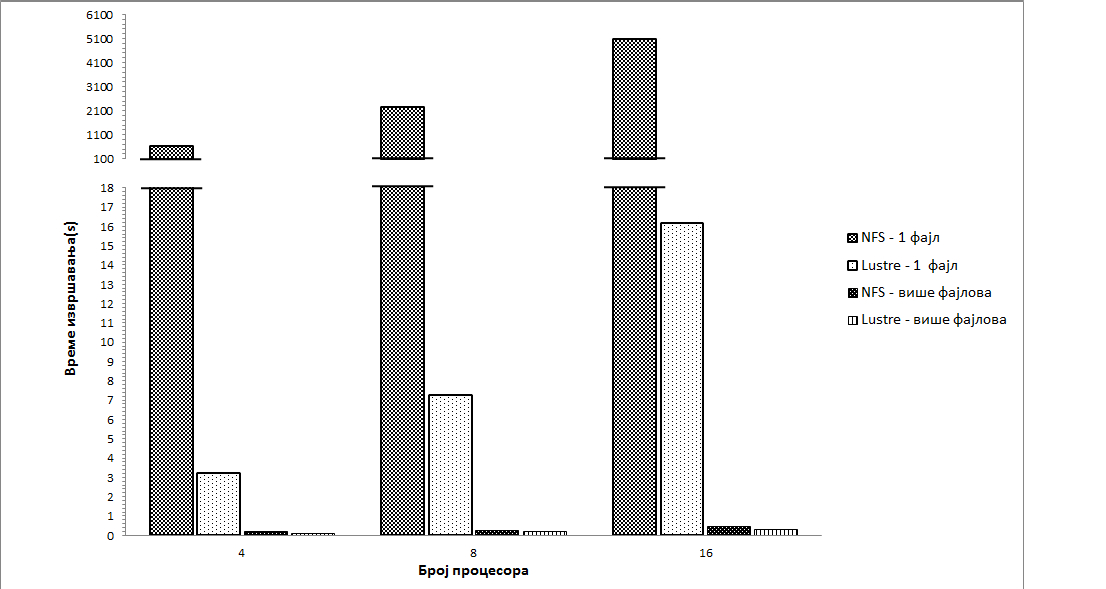
\includegraphics[width=1\textwidth]{slike/results/32_32.png}\\[1cm]
   \caption{Матрица 32x32, 32 итерација}
 \end{figure}
 
  \begin{figure}[H]
    \centering
        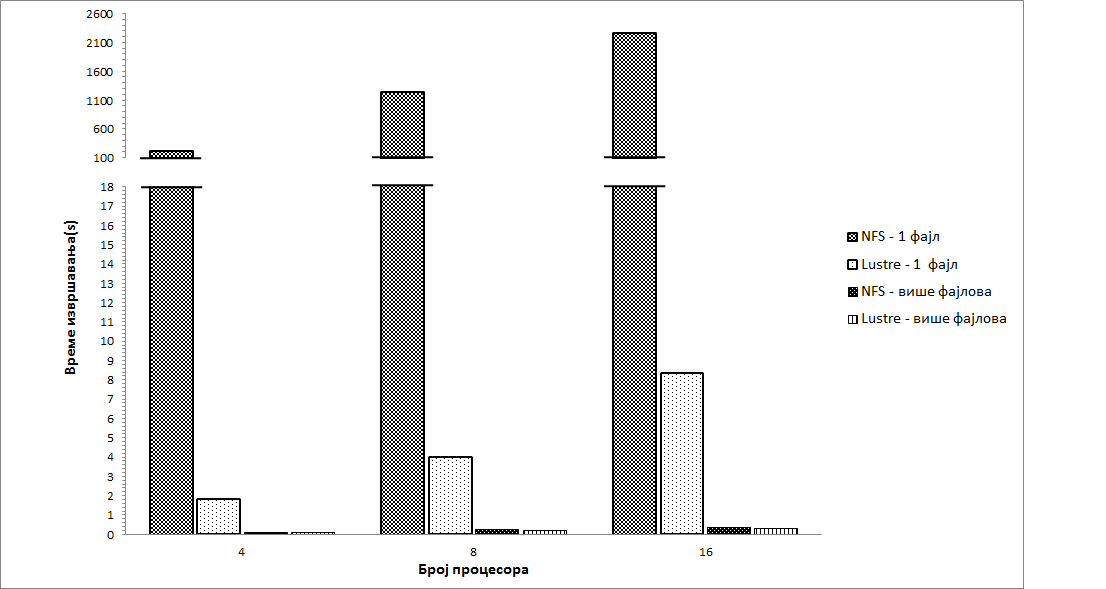
\includegraphics[width=1\textwidth]{slike/results/32_64.png}\\[1cm]
    \caption{Матрица 32x32, 64 итерација}
  \end{figure}
 
    \begin{figure}[H]
      \centering
          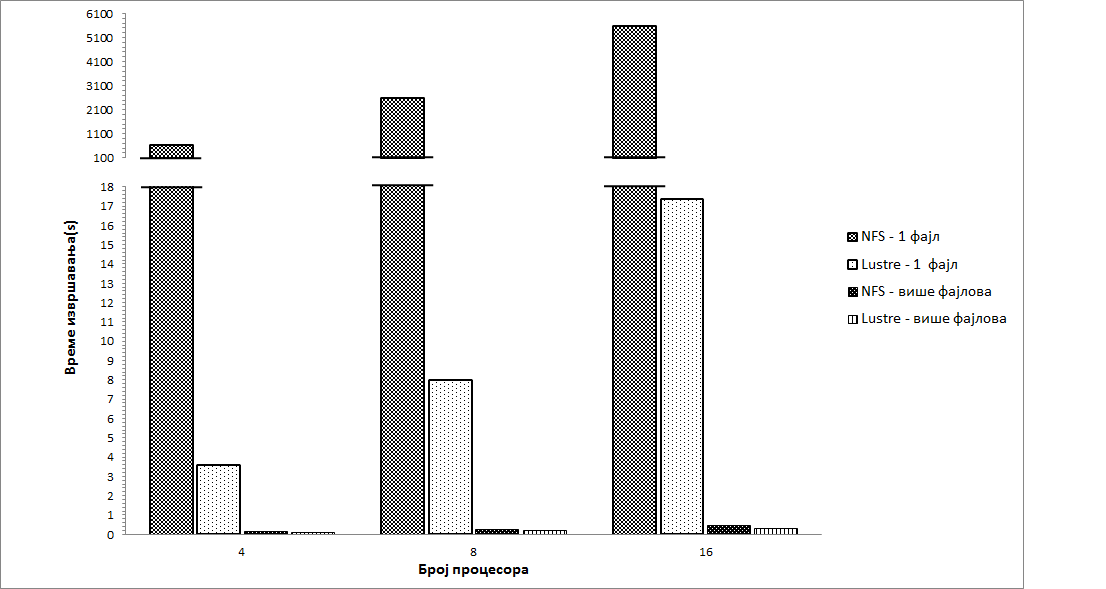
\includegraphics[width=1\textwidth]{slike/results/32_128.png}\\[1cm]
      \caption{Матрица 32x32, 128 итерација}
    \end{figure}
   
    \begin{figure}[H]
      \centering
          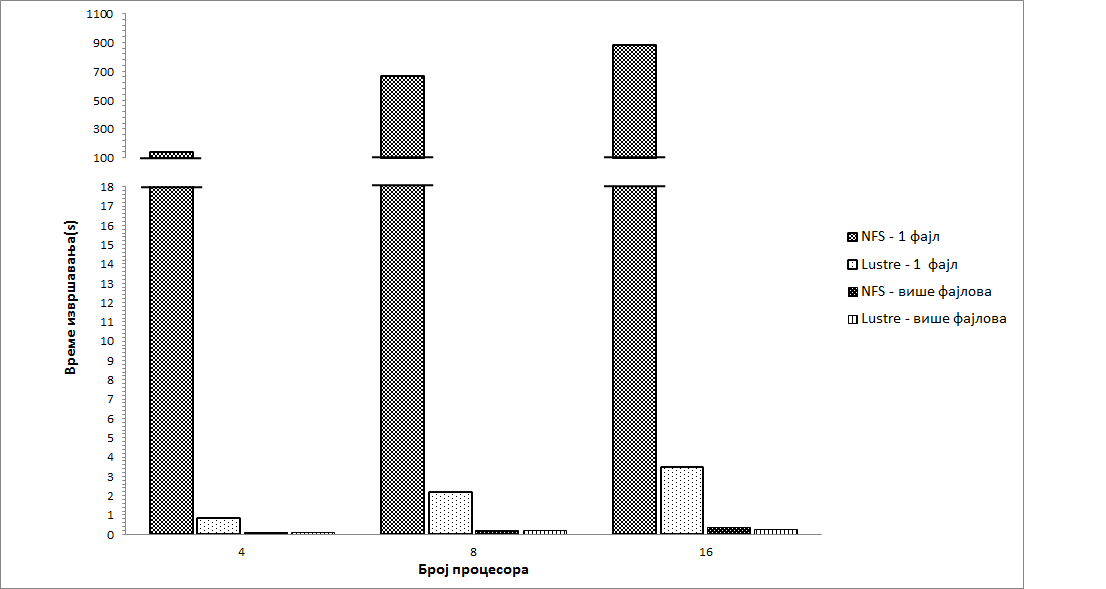
\includegraphics[width=1\textwidth]{slike/results/64_32.png}\\[1cm]
      \caption{Матрица 64x64, 32 итерација}
    \end{figure}
    
     \begin{figure}[H]
       \centering
           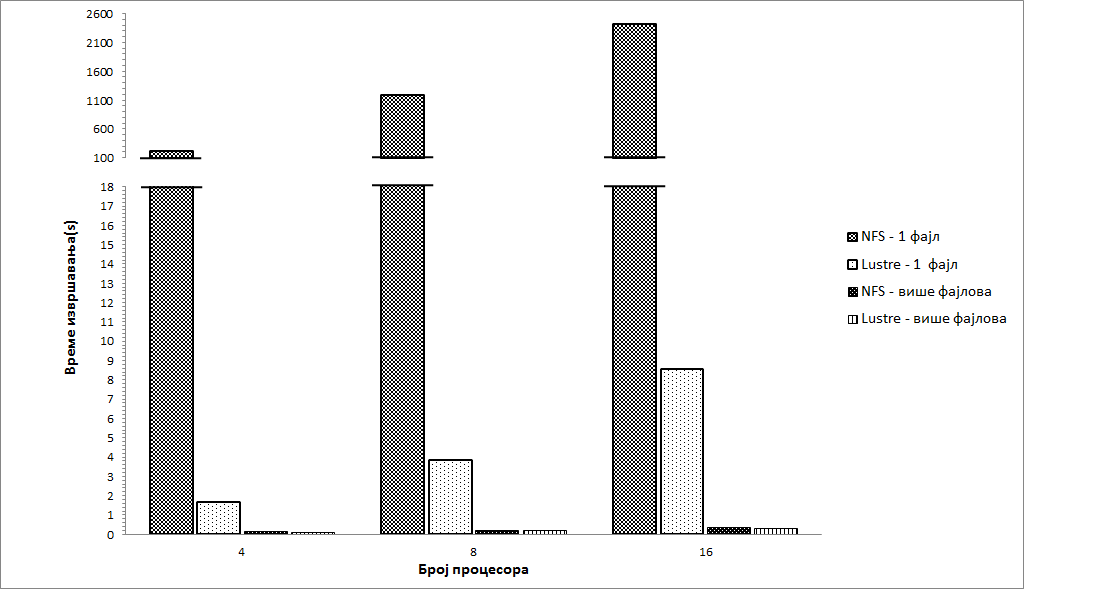
\includegraphics[width=1\textwidth]{slike/results/64_64.png}\\[1cm]
        \caption{Матрица 64x64, 64 итерација}
     \end{figure}
     
      \begin{figure}[H]
        \centering
            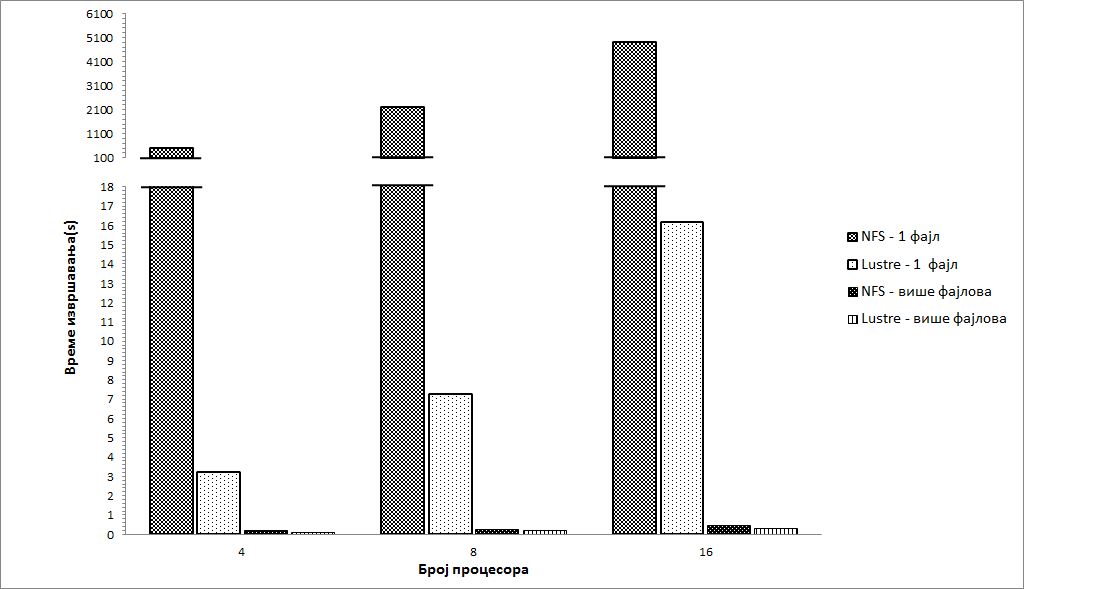
\includegraphics[width=1\textwidth]{slike/results/64_128.png}\\[1cm]
         \caption{Матрица 64x64, 128 итерација}
      \end{figure}
      
      \begin{figure}[H]
        \centering
            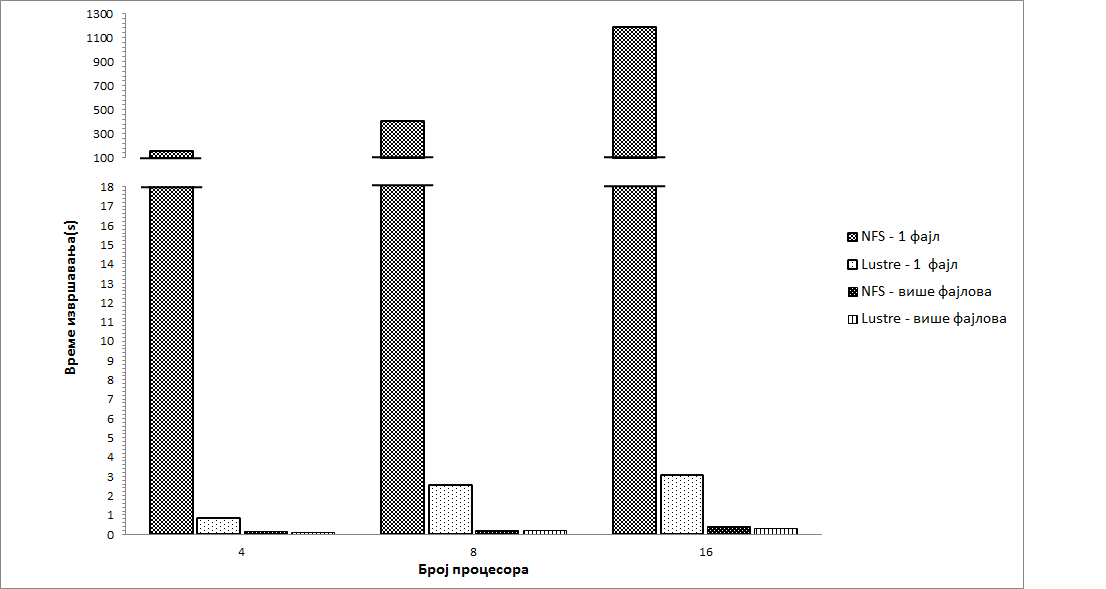
\includegraphics[width=1\textwidth]{slike/results/128_32.png}\\[1cm]
        \caption{Матрица 128x128, 32 итерација}
      \end{figure}
      
      \begin{figure}[H]
        \centering
            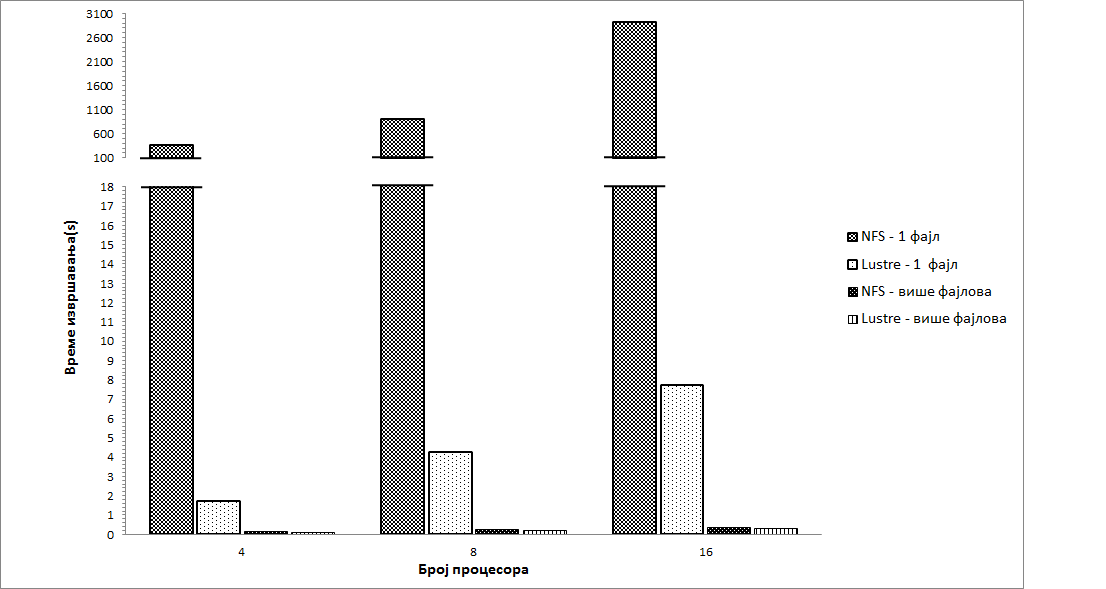
\includegraphics[width=1\textwidth]{slike/results/128_64.png}\\[1cm]
        \caption{Матрица 128x128, 64 итерација}
      \end{figure}
      
      \begin{figure}[H]
        \centering
            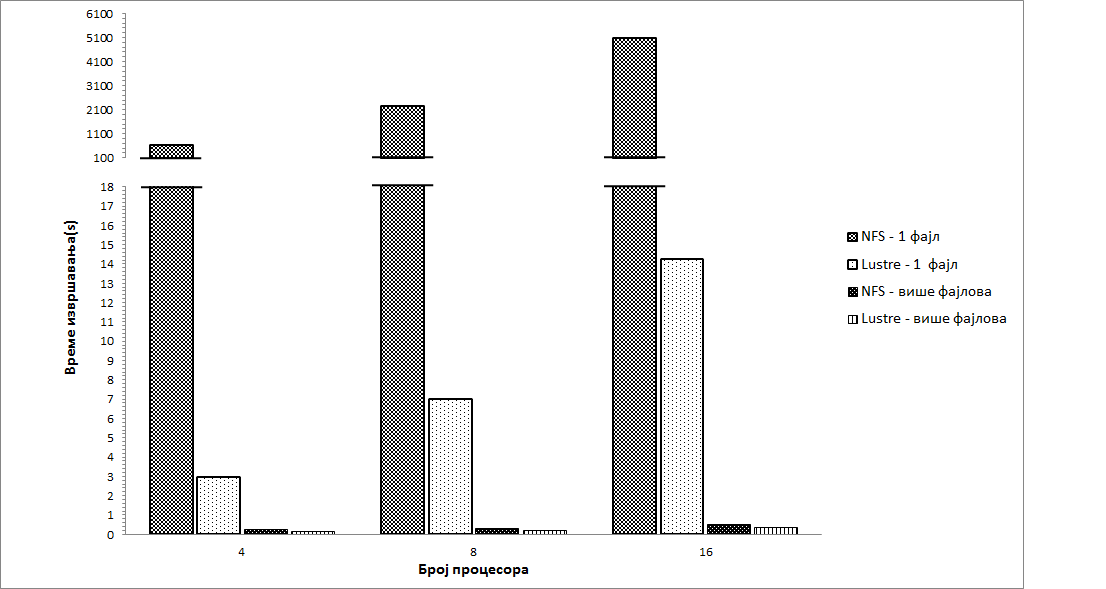
\includegraphics[width=1\textwidth]{slike/results/128_128.png}\\[1cm]
       \caption{Матрица 128x128, 128 итерација}
      \end{figure}
  
Од слике 4.7 до 4.15 приказано је време извршавања програма \textit{Game of Life} у зависности од комбинације параметара као што су: број процеса, величине матрице, број итерација и начин коришћења улазно/излазних операција. Уочава се да је време извршавања значајно мање код \textit{Lustre} фајл система, посебно када сваки процес има засебан фајл. Када сви процеси користе један фајл, \textit{Lustre} фајл систему је опет потребно мање времена него NFS фајл систему. Повећањем броја процеса ова разлика постаје уочљивија. 
Што је већа матрица и већи број итерација, то је количина података већа. Читањем и писањем већег броја података, \textit{Lustre} показује већу ефикасност. 
  
 
 
 
%
% Spisak Literature
%
\begin{thebibliography}{11}
\bibitem{egghead} {http://stormerider.com/wp-content/uploads/2011/05/820-7390.pdf, март 2014}
\bibitem{egghead} {http://docs.oracle.com/cd/E19527-01/821-2076-10/821-2076-10.pdf, мај 2014}
\bibitem{egghead} {http://linux.cloudibee.com/2009/11/lustre-cluster-filesystem-quick-setup-guide/, октобар 2014}
\bibitem{egghead} {https://www.kernel.org/doc/ols/2003/ols2003-pages-380-386.pdf, октобар 2014}
\bibitem{egghead} {http://imi.pmf.kg.ac.rs/moodle/file.php/127/Materijali\_za\_vezbe/2013\_14\_Primeri/13\_GOL.c, мaj 2015}
\bibitem{egghead} {http://www.conwaylife.com/wiki/Conway's\_Game\_of\_Life, мaj 2015}
\bibitem{egghead} {Using MPI-2 Advanced Features of the Message-Passing Interface, William Gropp, Ewing Lusk, Rajeev Thakur, 1999}
\bibitem{egghead} {MPI -- the Complete Reference. Vol. 2, The MPI-2 Extensions Scientific and Engineering Computation Series Gropp, William. MIT Press, 1998}
\bibitem{egghead} {MPI-2: Extensions to the Message-Passing Interface - Message Passing Interface Forum, 2009}
\bibitem{egghead} {Recent Advances in Parallel Virtual Machine and Message Passing Interface: 14th European PVM/MPI User's Group Meeting, Paris France, 2007}
\end{thebibliography}



\end{document}